%!TEX root = ../2015_06_16-HATS-LPC-JEC.tex

\subsection{Why?}
\frame{
	\frametitle{Introduction to Jet Energy Corrections in CMS}
	\vspace*{-0.24cm}
	\begin{columns}
		\begin{column}{0.49\textwidth}
			\begin{block}{Why do we need jet energy corrections?}
					\begin{itemize}
						\item For an abundance of reasons, the CMS detector does not perfectly measure the $p_{T}$ of most of the jets
						\item Therefore it is not straightforward to translate the measured jet energy to the true particle or parton energy
						\item Reasons:
						\begin{itemize}
							\item Pileup can add extra energy to the jets making their {\color{orange} response} ($p_{T}^{measured}/p_{T}^{actual}$) too high
							\item The calorimeter response to particles is not constant in either $p_{T}^{RECO}$ or $\eta$
							\item The detector response varies with jet flavor and parton flavor
							\item etc.
						\end{itemize}
					\end{itemize}
				\end{block}
		\end{column}
		\begin{column}{0.49\textwidth}
			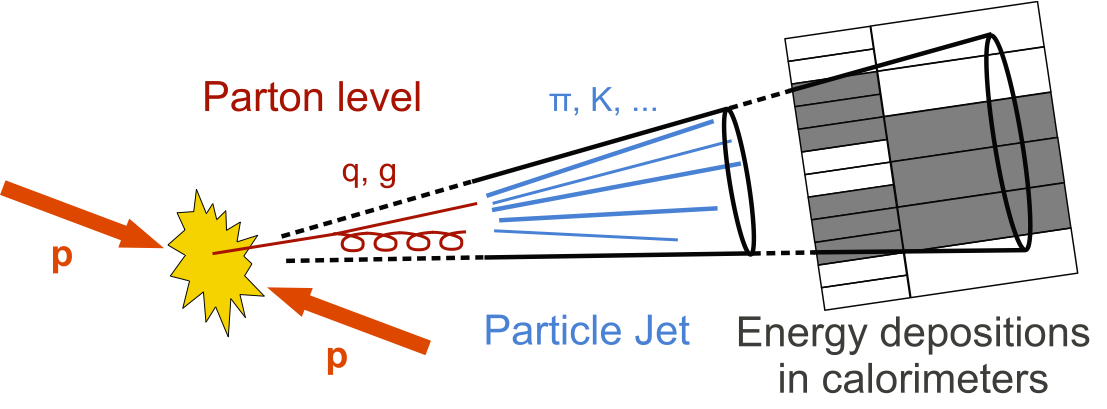
\includegraphics[width=\textwidth]{images/jetsatcmsand.png}\\
			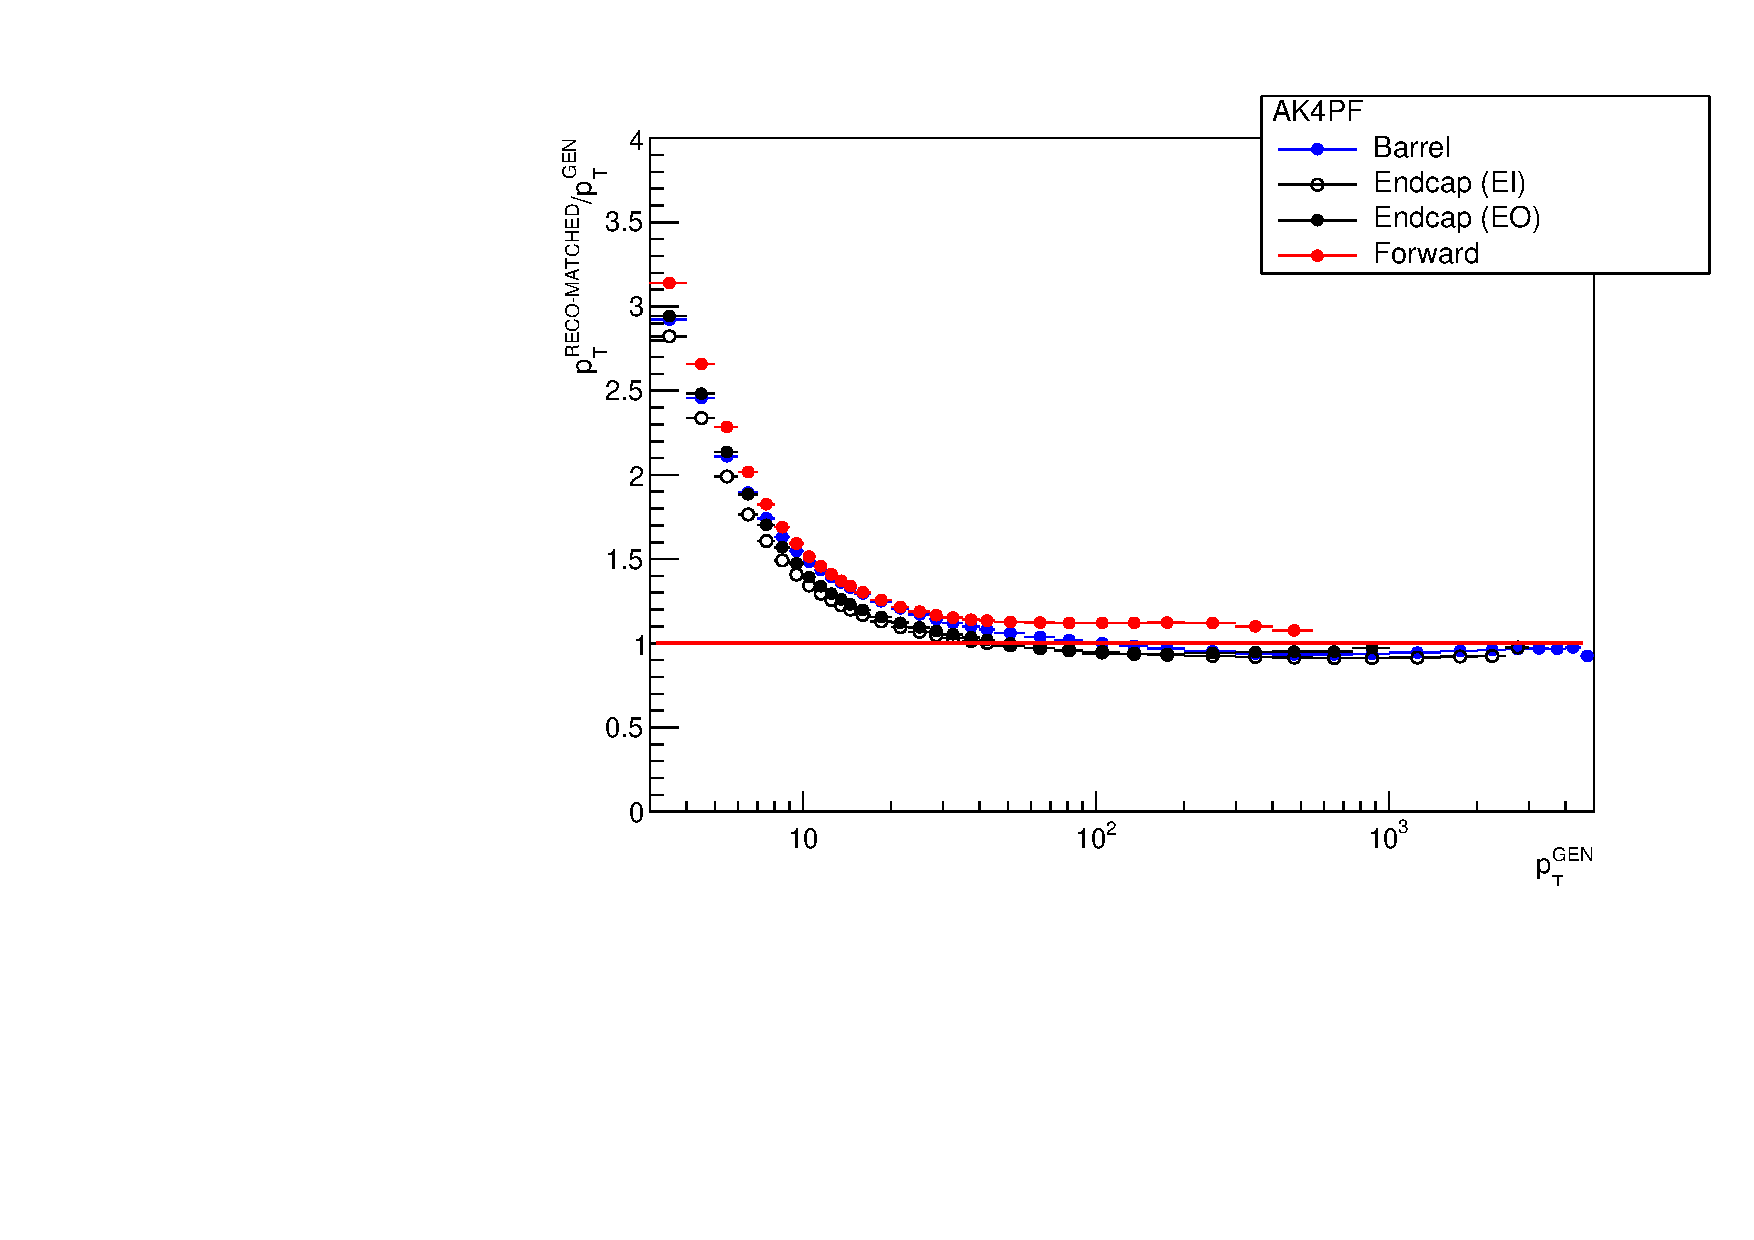
\includegraphics[width=\textwidth]{images/response.pdf}
		\end{column}
	\end{columns}
}

%---------------------------------------------------------------------------------------------------------------------------------------
\subsection{What?}
\frame{
	\frametitle{What are the JECs?}
	\vspace*{-0.24cm}
	\begin{block}{Definition}
		\begin{itemize}
			\item The jet energy corrections (JEC) are a set of functions, constants, and tools that allows the proper mapping of the measured jet energy to the energy of the initiating parton
		\end{itemize}
	\end{block}
	\vspace*{-0.15cm}
	\begin{block}{Factorized Approach}
		\begin{itemize}
			\item CMS has adopted a factorized solution to the problem of jet energy corrections, where each level of correction takes care of a different effect
			\begin{itemize}
				\item Each level of correction is essentially the application of a scale factor (correction) to the jet four momentum
				\item This scale factor depends on various event and jet related quantities ($\rho$, $p_{T}, \eta$, flavor, etc.)
				\item The levels of correction are applied sequentially (the output of each step is the input to the next) and with fixed order
			\end{itemize}
		\end{itemize}
	\end{block}
	\vspace*{-0.15cm}
	\begin{center}
		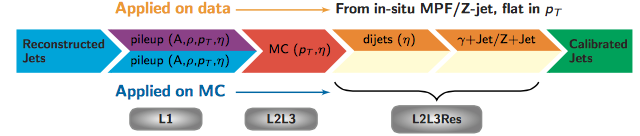
\includegraphics[width=10cm]{images/jecs.png}
	\end{center}
}
%---------------------------------------------------------------------------------------------------------------------------------------
\frame{
	\frametitle{JECs: A Factorized Approach}
%	\begin{textblock}{12.3}(0.25,0.7) %alexx
	\begin{textblock}{.9}(0.05,0.085) %ben
		\begin{figure}
			\scalebox{.9}{
			  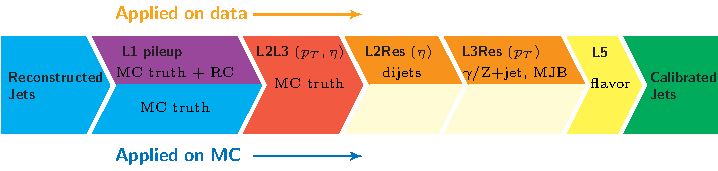
\includegraphics[width=\textwidth]{images/CMS_JEC_levels.pdf}
			}
			\label{fig:factorized_approach}
		\end{figure}
	\end{textblock}
	\vspace*{2.4cm}
	\begin{block}{Pileup (PU) Corrections}
		\begin{itemize}
			\footnotesize
			\item Pileup is the additional energy in a jet coming from all interactions \textbf{except} the primary vertex (PV) and it's underlying event (UE)
                          \begin{itemize}
                                \footnotesize
                                \item {\color{orange} Offset} $\equiv p_{T}^{with\ PU} - p_{T}^{no\ PU}$
                        \end{itemize}
			\item The goal of the pileup (\textbf{L1}) corrections is to remove the energy inside a jet coming from pile-up events
			\begin{itemize}
				\footnotesize
				\item L1Offset - No longer used
				\item L1FastJet - The current standard
				\item Charged Hardron Subtraction - Remove the charged hadrons inside a jet which have a track coming from a pileup vertex
				\item Pileup Per Particle Identification (PUPPI) - the new kid on the block 
			\end{itemize}
			\item Done on an {\color{blue}event-by-event} basis ($\rho$, $\mu$) and a {\color{red}jet-by-jet} basis ($p_{T}$, $\eta$, jet area)
			\item The first step in calculating these is MC based, but the corrections for data are scaled with L1Residual corrections
		\end{itemize}
	\end{block}
}
%---------------------------------------------------------------------------------------------------------------------------------------
\frame{
	\frametitle{JECs: A Factorized Approach}
        \begin{textblock}{.9}(0.05,0.085)
		\begin{figure}
			\scalebox{.9}{
			%	\documentclass[dvipsnames]{standalone}
\usepackage{color}
\usepackage{tikz}
\usetikzlibrary{arrows,shapes,shapes.multipart,backgrounds,calc,decorations.text,decorations.pathreplacing,matrix,shadings}
\tikzstyle{every picture}+=[remember picture]
\tikzstyle{na} = [baseline=-.5ex]

\begin{document}

\tikzstyle{levels} = [rectangle, draw, text width=6em, text centered, rounded corners, minimum height=2em, midway, shading=radial,outer color=Gray,middle color=white,inner color=white, Gray]
\tikzstyle{arrow} = [draw, -latex']
\tikzstyle{line} = [draw, -]

\newcommand*{\mytextstyle}{\sffamily\Large\bfseries\color{black!85}}
\newcommand{\myarrowstart}[9]{%
% inner radius, middle radius, outer radius, start angle,
% end angle, tip protusion angle, options, text
  \pgfmathsetmacro{\start}{#1}
  \pgfmathsetmacro{\rin}{#2}
  \pgfmathsetmacro{\rmid}{#3}
  \pgfmathsetmacro{\rout}{#4}
  \pgfmathsetmacro{\astart}{#5}
  \pgfmathsetmacro{\aend}{#6}
  \pgfmathsetmacro{\atip}{#7}
  \fill[#8] (\start+\astart,\rin) -- (\start+\aend,\rin) -- (\start+\aend+\atip,\rmid)
        -- (\start+\aend,\rout) -- (\start+\astart,\rout) -- (\start+\astart,\rmid)
        -- cycle;
  \node[font = \sffamily, align=center,text width=\aend-\astart,anchor = west, yshift=-0.0ex] (arrowend) at (\start+\astart,\rmid) {\mytextstyle{#9}};
%  \path[font = \sffamily, decoration = {text along path, text = {|\mytextstyle|#9},
%    text align = {align = center}, raise = -0.5ex}, decorate]
%    (\start+\astart+0.4*\atip,\rmid) -- (\start+\aend+0.4*\atip,\rmid);
}
\newcommand{\myarrow}[9]{%
% inner radius, middle radius, outer radius, start angle,
% end angle, tip protusion angle, options, text
  \pgfmathsetmacro{\start}{#1}
  \pgfmathsetmacro{\rin}{#2}
  \pgfmathsetmacro{\rmid}{#3}
  \pgfmathsetmacro{\rout}{#4}
  \pgfmathsetmacro{\astart}{#5}
  \pgfmathsetmacro{\aend}{#6}
  \pgfmathsetmacro{\atip}{#7}
  \fill[#8] (\start+\astart,\rin) -- (\start+\aend,\rin) -- (\start+\aend+\atip,\rmid) 
        -- (\start+\aend,\rout) -- (\start+\astart,\rout) -- (\start+\astart+\atip,\rmid)
        -- cycle;
  \path[font = \sffamily, decoration = {text along path, text = {|\mytextstyle|#9},
    text align = {align = center}, raise = -0.5ex}, decorate]
    (\start+\astart+0.75*\atip,\rmid) -- (\start+\aend+0.75*\atip,\rmid);
}
\newcommand{\myuphalfarrow}[9]{%
% inner radius, middle radius, outer radius, start angle,
% end angle, tip protusion angle, options, text
  \pgfmathsetmacro{\start}{#1}
  \pgfmathsetmacro{\rin}{#2}
  \pgfmathsetmacro{\rmid}{#3}
  \pgfmathsetmacro{\rout}{#4}
  \pgfmathsetmacro{\astart}{#5}
  \pgfmathsetmacro{\aend}{#6}
  \pgfmathsetmacro{\atip}{#7}
  \fill[#8] (\start+\astart,\rout) -- (\start+\aend,\rout) -- (\start+\aend+\atip,\rin) 
        -- (\start+\astart+\atip,\rin) -- cycle;
  \path[font = \sffamily, decoration = {text along path, text = {|\mytextstyle|#9},
    text align = {align = center}, raise = -0.5ex}, decorate]
    (\start+\astart+0.4*\atip,\rmid) -- (\start+\aend+0.4*\atip,\rmid);
}
\newcommand{\mylowhalfarrow}[9]{%
% inner radius, middle radius, outer radius, start angle,
% end angle, tip protusion angle, options, text
  \pgfmathsetmacro{\start}{#1}
  \pgfmathsetmacro{\rin}{#2}
  \pgfmathsetmacro{\rmid}{#3}
  \pgfmathsetmacro{\rout}{#4}
  \pgfmathsetmacro{\astart}{#5}
  \pgfmathsetmacro{\aend}{#6}
  \pgfmathsetmacro{\atip}{#7}
  \fill[#8] (\start+\astart+\atip,\rin) -- (\start+\aend+\atip,\rin) -- (\start+\aend,\rout)
        -- (\start+\astart,\rout) -- cycle;
  \path[font = \sffamily, decoration = {text along path, text = {|\mytextstyle|#9},
    text align = {align = center}, raise = -0.5ex}, decorate]
    (\start+\astart+0.4*\atip,\rmid) -- (\start+\aend+0.4*\atip,\rmid);
}
\newcommand{\myarrowend}[9]{%
% inner radius, middle radius, outer radius, start angle,
% end angle, tip protusion angle, options, text
  \pgfmathsetmacro{\start}{#1}
  \pgfmathsetmacro{\rin}{#2}
  \pgfmathsetmacro{\rmid}{#3}
  \pgfmathsetmacro{\rout}{#4}
  \pgfmathsetmacro{\astart}{#5}
  \pgfmathsetmacro{\aend}{#6}
  \pgfmathsetmacro{\atip}{#7}
  \fill[#8] (\start+\astart,\rin) -- (\start+\aend,\rin) -- (\start+\aend,\rmid)
        -- (\start+\aend,\rout) -- (\start+\astart,\rout) -- (\start+\astart+\atip,\rmid)
        -- cycle;
  \node[font = \sffamily, align=center,text width=\aend-\astart,anchor = west, yshift=-0.0ex] (arrowend) at (\start+\astart+0.75*\atip,\rmid) {\mytextstyle{#9}};
}

\begin{tikzpicture}[node distance = 2cm, auto, scale=0.8]
\scriptsize
    % Place nodes
    \myarrowstart{0}{0.5}{1.5}{2.5}{0}{1.75}{0.5}{Cyan,draw = Cyan, very thick}{\scriptsize{Reconstructed Jets}}

    \myuphalfarrow{1.95}{1.52}{1.75}{2.5}{0}{2.0}{0.5}{Purple,draw = Purple, very thick}{|\scriptsize|{MC + RC}}
    \mylowhalfarrow{1.95}{1.48}{1.}{0.5}{0}{2.0}{0.5}{Cyan,draw = Cyan, very thick}{|\scriptsize|{MC}}

    \node [font = \sffamily, align=left,text width=2.cm,anchor = west, yshift=-0.0ex] (l1data) at (2.4,2.2) {\mytextstyle\small\color{Black}\scriptsize{Pileup}};


    \myarrow{4.15}{0.5}{1.5}{2.5}{0}{2.95}{0.5}{Red!80,draw = Red!80, very thick}{|\scriptsize|{MC}}
    \node [font = \sffamily, align=left,text width=2.cm,anchor = west, yshift=-0.0ex] (l2l3) at (4.35,2.2) {\mytextstyle\small\color{Black}\scriptsize{Response $(p_{T},\eta)$ }};


    \myuphalfarrow{7.3}{1.52}{1.75}{2.5}{0}{1.9}{0.5}{BurntOrange,draw = BurntOrange, very thick}{|\scriptsize|{dijets}}
    \node [font = \sffamily, align=left,text width=2.cm,anchor = west, yshift=-0.0ex] (l2res) at (7.4,2.2) {\mytextstyle\small\color{Black}\scriptsize{Residuals$(\eta)$}};
    \mylowhalfarrow{7.3}{1.48}{1.25}{0.5}{0}{1.9}{0.5}{yellow!20,draw = yellow!20, very thick}{}


   \myuphalfarrow{9.4}{1.52}{1.75}{2.5}{0}{2.4}{0.5}{BurntOrange,draw = BurntOrange, very thick}{|\scriptsize|{   $\gamma$/Z$+$jet, MJB}}
    \node [font = \sffamily, align=left,text width=2.cm,anchor = west, yshift=-0.0ex] (l3res) at (9.6,2.2) {\mytextstyle\small\color{Black}\scriptsize{Residuals$(p_T)$}};
    \mylowhalfarrow{9.4}{1.48}{1.25}{0.5}{0}{2.4}{0.5}{yellow!20,draw = yellow!20, very thick}{}

 
   \myarrow{12.0}{0.5}{1.5}{2.5}{0}{1.}{0.5}{Yellow!80,draw = Yellow!80, very thick}{|\scriptsize|{MC}}
    \node [font = \sffamily, align=left,text width=2.cm,anchor = west, yshift=-0.0ex] (l5) at (12.,2.2) {\mytextstyle\small\color{Black}\scriptsize{ Flavor}};


    \myarrowend{13.20}{0.5}{1.5}{2.5}{0}{2.}{0.5}{Green!90,draw = Green!90, very thick}{\scriptsize{Calibrated Jets}}
    
    \node [font = \sffamily, align=left,text width=2.75cm,anchor = west, yshift=-0.0ex] (MC) at (2.25,0.) {\mytextstyle\small\color{RoyalBlue}Applied on MC};
    \node [font = \sffamily, align=left,text width=2.75cm,anchor = west, yshift=-0.0ex] (DATA) at (2.25,3.) {\mytextstyle\small\color{YellowOrange}Applied on data};

    \node [font = \sffamily, align=left,text width=5cm,anchor = west, yshift=-0.0ex] (INSITU) at (7.6,3.) %%{\mytextstyle\footnotesize{From in-situ MPF/Z-jet, flat in $p_{T}$}};
   {\mytextstyle\footnotesize{}};
    \node [font = \sffamily, align=left,text width=5cm,anchor = west, yshift=-0.0ex] (STARTBRACE) at (7.6,0.) {};
    \node [font = \sffamily, align=left,text width=5cm,anchor = west, yshift=-0.0ex] (ENDBRACE) at (12.65,0.5) {};
    \path[arrow,YellowOrange,thick, shorten <= -0.5cm] (DATA) -- (INSITU);
%    \draw [thick, decorate, decoration = {brace, amplitude = 10pt, mirror}, xshift = 0pt, yshift = 0pt] (7.25,0.75) -- (12.0,0.75) node [black, midway, xshift = 0cm, yshift = -0.8cm] {\mytextstyle\small{stuff}};
 %   \draw [thick, decorate, decoration = {brace, amplitude = 10pt, mirror}, xshift = 0pt, yshift = 0pt] (7.7,0.75) -- (12.65,0.75) node [levels, xshift = 0cm, yshift = -1.0cm] {\mytextstyle\scriptsize{L2L3Res}};

   \path[arrow,RoyalBlue,thick, shorten <= -0.5cm] (MC) -- (STARTBRACE);

 %   \node [levels, below of=MC, xshift = 3.6cm, yshift = 1.85cm, thick] (L1) {\mytextstyle\small{L1}};
 %   \node [levels, right of=L1, xshift = 4.4cm, yshift = -0.15cm, thick] (L2L3) {\mytextstyle\small{L2L3}};
\end{tikzpicture}

\end{document}

				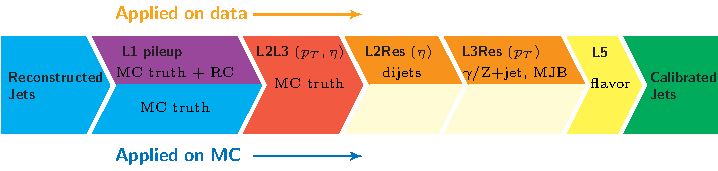
\includegraphics[width=\textwidth]{images/CMS_JEC_levels.pdf}
			}
			\label{fig:factorized_approach}
		\end{figure}
	\end{textblock}
	\vspace*{2.4cm}
	\begin{block}{Pileup (PU) Corrections}
		\begin{itemize}
			\footnotesize
			\item Pileup is the additional energy in a jet coming from all interactions \textbf{except} the primary vertex (PV) and it's underlying event (UE)
			\item The goal of the pileup (\textbf{L1}) corrections is to remove the energy inside a jet coming from pile-up events
			\begin{itemize}
				\footnotesize
				\item L1Offset - No longer used
				\item L1FastJet - The current standard
				\item Charged Hardron Subtraction - Remove the charged hadrons inside a jet which have a track coming from a pileup vertex
				\item Pileup Per Particle Identification (PUPPI) - the new kid on the block
			\end{itemize}
			\item Done on an {\color{blue}event-by-event} basis ($\rho$, $\mu$) and a {\color{red}jet-by-jet} basis ($p_{T}$, $\eta$, jet area)
			\item The first step in calculating these is MC based, but the corrections for data are scaled with L1Residual corrections
		\end{itemize}
	\end{block}
	\begin{textblock}{.9}(0.05,.25)
		\begin{figure}
			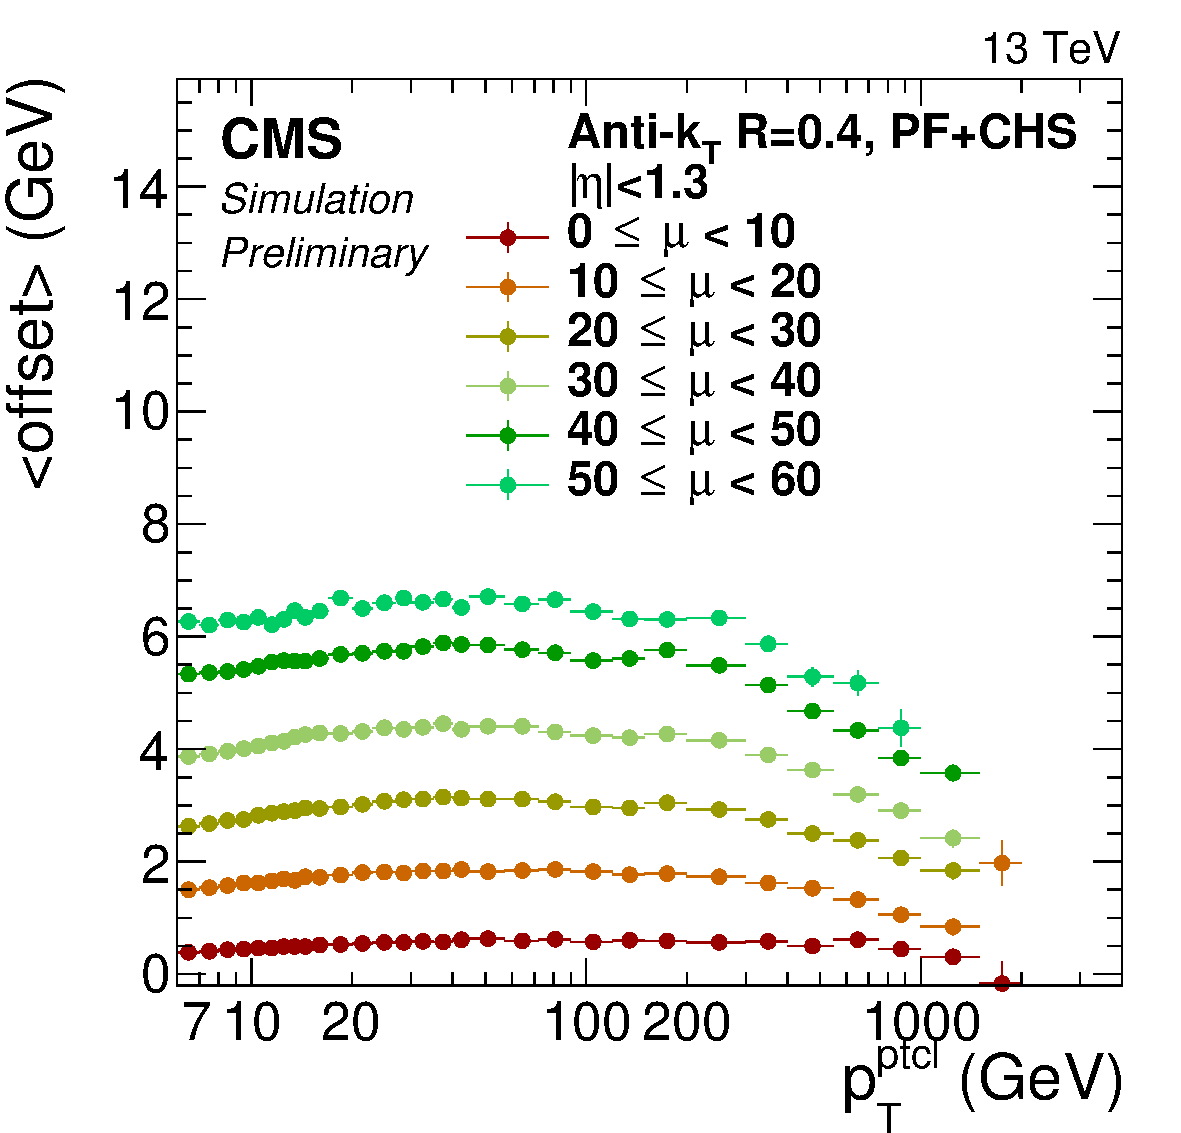
\includegraphics[width=0.5\textwidth]{images/JME-16-001/OffMeantnpuRef_BB_ak4pfchs_no2000_beforeL1.pdf}
			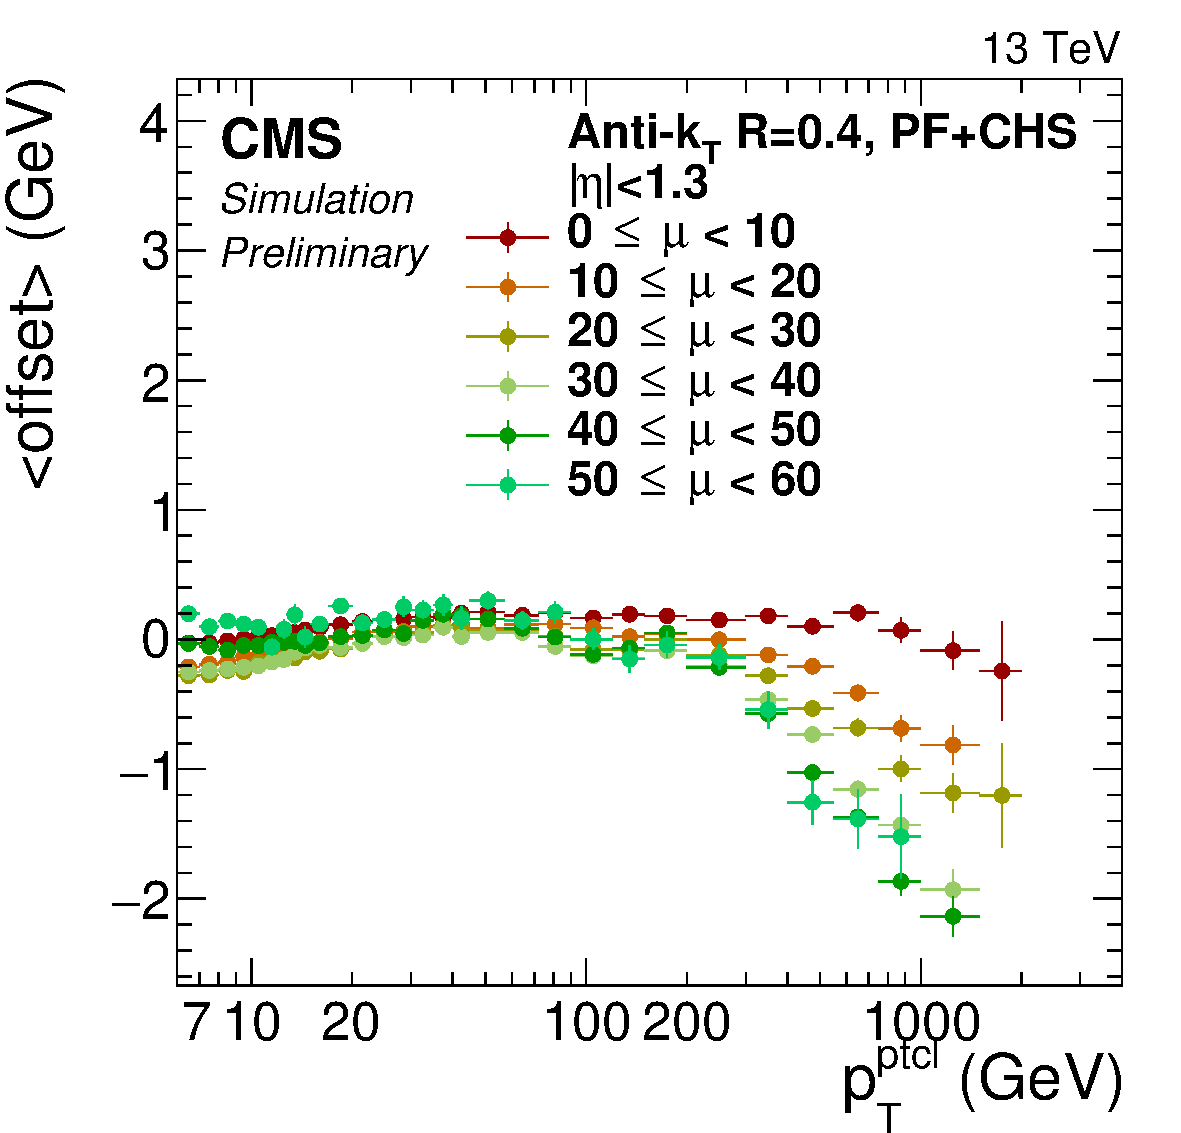
\includegraphics[width=0.5\textwidth]{images/JME-16-001/OffMeantnpuRef_BB_ak4pfchs_no2000_afterL1.pdf}
			\label{fig:OffMeantnpuRef}
		\end{figure}
	\end{textblock}
}
%---------------------------------------------------------------------------------------------------------------------------------------
\frame{
	\frametitle{JECs: A Factorized Approach}
        \begin{textblock}{.9}(0.05,0.085)
		\begin{figure}
			\scalebox{.9}{
			%	\documentclass[dvipsnames]{standalone}
\usepackage{color}
\usepackage{tikz}
\usetikzlibrary{arrows,shapes,shapes.multipart,backgrounds,calc,decorations.text,decorations.pathreplacing,matrix,shadings}
\tikzstyle{every picture}+=[remember picture]
\tikzstyle{na} = [baseline=-.5ex]

\begin{document}

\tikzstyle{levels} = [rectangle, draw, text width=6em, text centered, rounded corners, minimum height=2em, midway, shading=radial,outer color=Gray,middle color=white,inner color=white, Gray]
\tikzstyle{arrow} = [draw, -latex']
\tikzstyle{line} = [draw, -]

\newcommand*{\mytextstyle}{\sffamily\Large\bfseries\color{black!85}}
\newcommand{\myarrowstart}[9]{%
% inner radius, middle radius, outer radius, start angle,
% end angle, tip protusion angle, options, text
  \pgfmathsetmacro{\start}{#1}
  \pgfmathsetmacro{\rin}{#2}
  \pgfmathsetmacro{\rmid}{#3}
  \pgfmathsetmacro{\rout}{#4}
  \pgfmathsetmacro{\astart}{#5}
  \pgfmathsetmacro{\aend}{#6}
  \pgfmathsetmacro{\atip}{#7}
  \fill[#8] (\start+\astart,\rin) -- (\start+\aend,\rin) -- (\start+\aend+\atip,\rmid)
        -- (\start+\aend,\rout) -- (\start+\astart,\rout) -- (\start+\astart,\rmid)
        -- cycle;
  \node[font = \sffamily, align=center,text width=\aend-\astart,anchor = west, yshift=-0.0ex] (arrowend) at (\start+\astart,\rmid) {\mytextstyle{#9}};
%  \path[font = \sffamily, decoration = {text along path, text = {|\mytextstyle|#9},
%    text align = {align = center}, raise = -0.5ex}, decorate]
%    (\start+\astart+0.4*\atip,\rmid) -- (\start+\aend+0.4*\atip,\rmid);
}
\newcommand{\myarrow}[9]{%
% inner radius, middle radius, outer radius, start angle,
% end angle, tip protusion angle, options, text
  \pgfmathsetmacro{\start}{#1}
  \pgfmathsetmacro{\rin}{#2}
  \pgfmathsetmacro{\rmid}{#3}
  \pgfmathsetmacro{\rout}{#4}
  \pgfmathsetmacro{\astart}{#5}
  \pgfmathsetmacro{\aend}{#6}
  \pgfmathsetmacro{\atip}{#7}
  \fill[#8] (\start+\astart,\rin) -- (\start+\aend,\rin) -- (\start+\aend+\atip,\rmid) 
        -- (\start+\aend,\rout) -- (\start+\astart,\rout) -- (\start+\astart+\atip,\rmid)
        -- cycle;
  \path[font = \sffamily, decoration = {text along path, text = {|\mytextstyle|#9},
    text align = {align = center}, raise = -0.5ex}, decorate]
    (\start+\astart+0.75*\atip,\rmid) -- (\start+\aend+0.75*\atip,\rmid);
}
\newcommand{\myuphalfarrow}[9]{%
% inner radius, middle radius, outer radius, start angle,
% end angle, tip protusion angle, options, text
  \pgfmathsetmacro{\start}{#1}
  \pgfmathsetmacro{\rin}{#2}
  \pgfmathsetmacro{\rmid}{#3}
  \pgfmathsetmacro{\rout}{#4}
  \pgfmathsetmacro{\astart}{#5}
  \pgfmathsetmacro{\aend}{#6}
  \pgfmathsetmacro{\atip}{#7}
  \fill[#8] (\start+\astart,\rout) -- (\start+\aend,\rout) -- (\start+\aend+\atip,\rin) 
        -- (\start+\astart+\atip,\rin) -- cycle;
  \path[font = \sffamily, decoration = {text along path, text = {|\mytextstyle|#9},
    text align = {align = center}, raise = -0.5ex}, decorate]
    (\start+\astart+0.4*\atip,\rmid) -- (\start+\aend+0.4*\atip,\rmid);
}
\newcommand{\mylowhalfarrow}[9]{%
% inner radius, middle radius, outer radius, start angle,
% end angle, tip protusion angle, options, text
  \pgfmathsetmacro{\start}{#1}
  \pgfmathsetmacro{\rin}{#2}
  \pgfmathsetmacro{\rmid}{#3}
  \pgfmathsetmacro{\rout}{#4}
  \pgfmathsetmacro{\astart}{#5}
  \pgfmathsetmacro{\aend}{#6}
  \pgfmathsetmacro{\atip}{#7}
  \fill[#8] (\start+\astart+\atip,\rin) -- (\start+\aend+\atip,\rin) -- (\start+\aend,\rout)
        -- (\start+\astart,\rout) -- cycle;
  \path[font = \sffamily, decoration = {text along path, text = {|\mytextstyle|#9},
    text align = {align = center}, raise = -0.5ex}, decorate]
    (\start+\astart+0.4*\atip,\rmid) -- (\start+\aend+0.4*\atip,\rmid);
}
\newcommand{\myarrowend}[9]{%
% inner radius, middle radius, outer radius, start angle,
% end angle, tip protusion angle, options, text
  \pgfmathsetmacro{\start}{#1}
  \pgfmathsetmacro{\rin}{#2}
  \pgfmathsetmacro{\rmid}{#3}
  \pgfmathsetmacro{\rout}{#4}
  \pgfmathsetmacro{\astart}{#5}
  \pgfmathsetmacro{\aend}{#6}
  \pgfmathsetmacro{\atip}{#7}
  \fill[#8] (\start+\astart,\rin) -- (\start+\aend,\rin) -- (\start+\aend,\rmid)
        -- (\start+\aend,\rout) -- (\start+\astart,\rout) -- (\start+\astart+\atip,\rmid)
        -- cycle;
  \node[font = \sffamily, align=center,text width=\aend-\astart,anchor = west, yshift=-0.0ex] (arrowend) at (\start+\astart+0.75*\atip,\rmid) {\mytextstyle{#9}};
}

\begin{tikzpicture}[node distance = 2cm, auto, scale=0.8]
\scriptsize
    % Place nodes
    \myarrowstart{0}{0.5}{1.5}{2.5}{0}{1.75}{0.5}{Cyan,draw = Cyan, very thick}{\scriptsize{Reconstructed Jets}}

    \myuphalfarrow{1.95}{1.52}{1.75}{2.5}{0}{2.0}{0.5}{Purple,draw = Purple, very thick}{|\scriptsize|{MC + RC}}
    \mylowhalfarrow{1.95}{1.48}{1.}{0.5}{0}{2.0}{0.5}{Cyan,draw = Cyan, very thick}{|\scriptsize|{MC}}

    \node [font = \sffamily, align=left,text width=2.cm,anchor = west, yshift=-0.0ex] (l1data) at (2.4,2.2) {\mytextstyle\small\color{Black}\scriptsize{Pileup}};


    \myarrow{4.15}{0.5}{1.5}{2.5}{0}{2.95}{0.5}{Red!80,draw = Red!80, very thick}{|\scriptsize|{MC}}
    \node [font = \sffamily, align=left,text width=2.cm,anchor = west, yshift=-0.0ex] (l2l3) at (4.35,2.2) {\mytextstyle\small\color{Black}\scriptsize{Response $(p_{T},\eta)$ }};


    \myuphalfarrow{7.3}{1.52}{1.75}{2.5}{0}{1.9}{0.5}{BurntOrange,draw = BurntOrange, very thick}{|\scriptsize|{dijets}}
    \node [font = \sffamily, align=left,text width=2.cm,anchor = west, yshift=-0.0ex] (l2res) at (7.4,2.2) {\mytextstyle\small\color{Black}\scriptsize{Residuals$(\eta)$}};
    \mylowhalfarrow{7.3}{1.48}{1.25}{0.5}{0}{1.9}{0.5}{yellow!20,draw = yellow!20, very thick}{}


   \myuphalfarrow{9.4}{1.52}{1.75}{2.5}{0}{2.4}{0.5}{BurntOrange,draw = BurntOrange, very thick}{|\scriptsize|{   $\gamma$/Z$+$jet, MJB}}
    \node [font = \sffamily, align=left,text width=2.cm,anchor = west, yshift=-0.0ex] (l3res) at (9.6,2.2) {\mytextstyle\small\color{Black}\scriptsize{Residuals$(p_T)$}};
    \mylowhalfarrow{9.4}{1.48}{1.25}{0.5}{0}{2.4}{0.5}{yellow!20,draw = yellow!20, very thick}{}

 
   \myarrow{12.0}{0.5}{1.5}{2.5}{0}{1.}{0.5}{Yellow!80,draw = Yellow!80, very thick}{|\scriptsize|{MC}}
    \node [font = \sffamily, align=left,text width=2.cm,anchor = west, yshift=-0.0ex] (l5) at (12.,2.2) {\mytextstyle\small\color{Black}\scriptsize{ Flavor}};


    \myarrowend{13.20}{0.5}{1.5}{2.5}{0}{2.}{0.5}{Green!90,draw = Green!90, very thick}{\scriptsize{Calibrated Jets}}
    
    \node [font = \sffamily, align=left,text width=2.75cm,anchor = west, yshift=-0.0ex] (MC) at (2.25,0.) {\mytextstyle\small\color{RoyalBlue}Applied on MC};
    \node [font = \sffamily, align=left,text width=2.75cm,anchor = west, yshift=-0.0ex] (DATA) at (2.25,3.) {\mytextstyle\small\color{YellowOrange}Applied on data};

    \node [font = \sffamily, align=left,text width=5cm,anchor = west, yshift=-0.0ex] (INSITU) at (7.6,3.) %%{\mytextstyle\footnotesize{From in-situ MPF/Z-jet, flat in $p_{T}$}};
   {\mytextstyle\footnotesize{}};
    \node [font = \sffamily, align=left,text width=5cm,anchor = west, yshift=-0.0ex] (STARTBRACE) at (7.6,0.) {};
    \node [font = \sffamily, align=left,text width=5cm,anchor = west, yshift=-0.0ex] (ENDBRACE) at (12.65,0.5) {};
    \path[arrow,YellowOrange,thick, shorten <= -0.5cm] (DATA) -- (INSITU);
%    \draw [thick, decorate, decoration = {brace, amplitude = 10pt, mirror}, xshift = 0pt, yshift = 0pt] (7.25,0.75) -- (12.0,0.75) node [black, midway, xshift = 0cm, yshift = -0.8cm] {\mytextstyle\small{stuff}};
 %   \draw [thick, decorate, decoration = {brace, amplitude = 10pt, mirror}, xshift = 0pt, yshift = 0pt] (7.7,0.75) -- (12.65,0.75) node [levels, xshift = 0cm, yshift = -1.0cm] {\mytextstyle\scriptsize{L2L3Res}};

   \path[arrow,RoyalBlue,thick, shorten <= -0.5cm] (MC) -- (STARTBRACE);

 %   \node [levels, below of=MC, xshift = 3.6cm, yshift = 1.85cm, thick] (L1) {\mytextstyle\small{L1}};
 %   \node [levels, right of=L1, xshift = 4.4cm, yshift = -0.15cm, thick] (L2L3) {\mytextstyle\small{L2L3}};
\end{tikzpicture}

\end{document}

				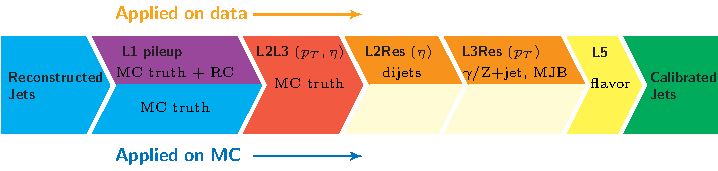
\includegraphics[width=\textwidth]{images/CMS_JEC_levels.pdf}
			}
			\label{fig:factorized_approach}
		\end{figure}
	\end{textblock}
	\vspace*{2.4cm}
	\begin{block}{Pileup (PU) Corrections}
		\begin{itemize}
			\footnotesize
			\item Pileup is the additional energy in a jet coming from all interactions \textbf{except} the primary vertex (PV) and it's underlying event (UE)
			\item The goal of the pileup (\textbf{L1}) corrections is to remove the energy inside a jet coming from pile-up events
			\begin{itemize}
				\footnotesize
				\item L1Offset - No longer used
				\item L1FastJet - The current standard
				\item Charged Hardron Subtraction - Remove the charged hadrons inside a jet which have a track coming from a pileup vertex
				\item Pileup Per Particle Identification (PUPPI) - the new kid on the block 
			\end{itemize}
			\item Done on an {\color{blue}event-by-event} basis ($\rho$, $\mu$) and a {\color{red}jet-by-jet} basis ($p_{T}$, $\eta$, jet area)
			\item The first step in calculating these is MC based, but the corrections for data are scaled with L1Residual corrections
		\end{itemize}
	\end{block}
	\begin{textblock}{.9}(0.05,.25)
		\begin{figure}
                        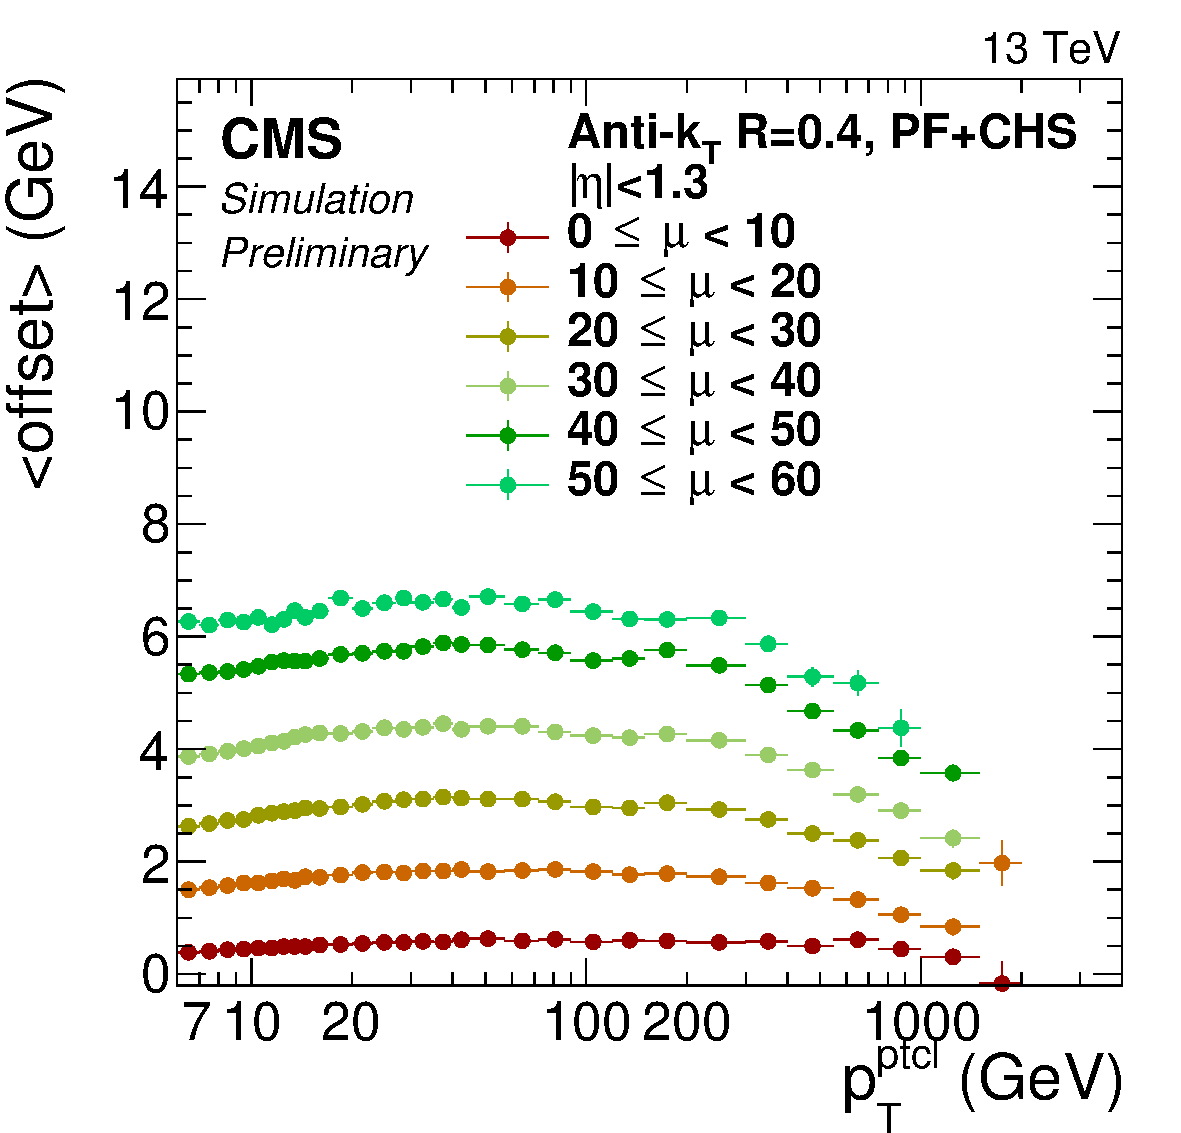
\includegraphics[width=0.5\textwidth]{images/JME-16-001/OffMeantnpuRef_BB_ak4pfchs_no2000_beforeL1.pdf}
                        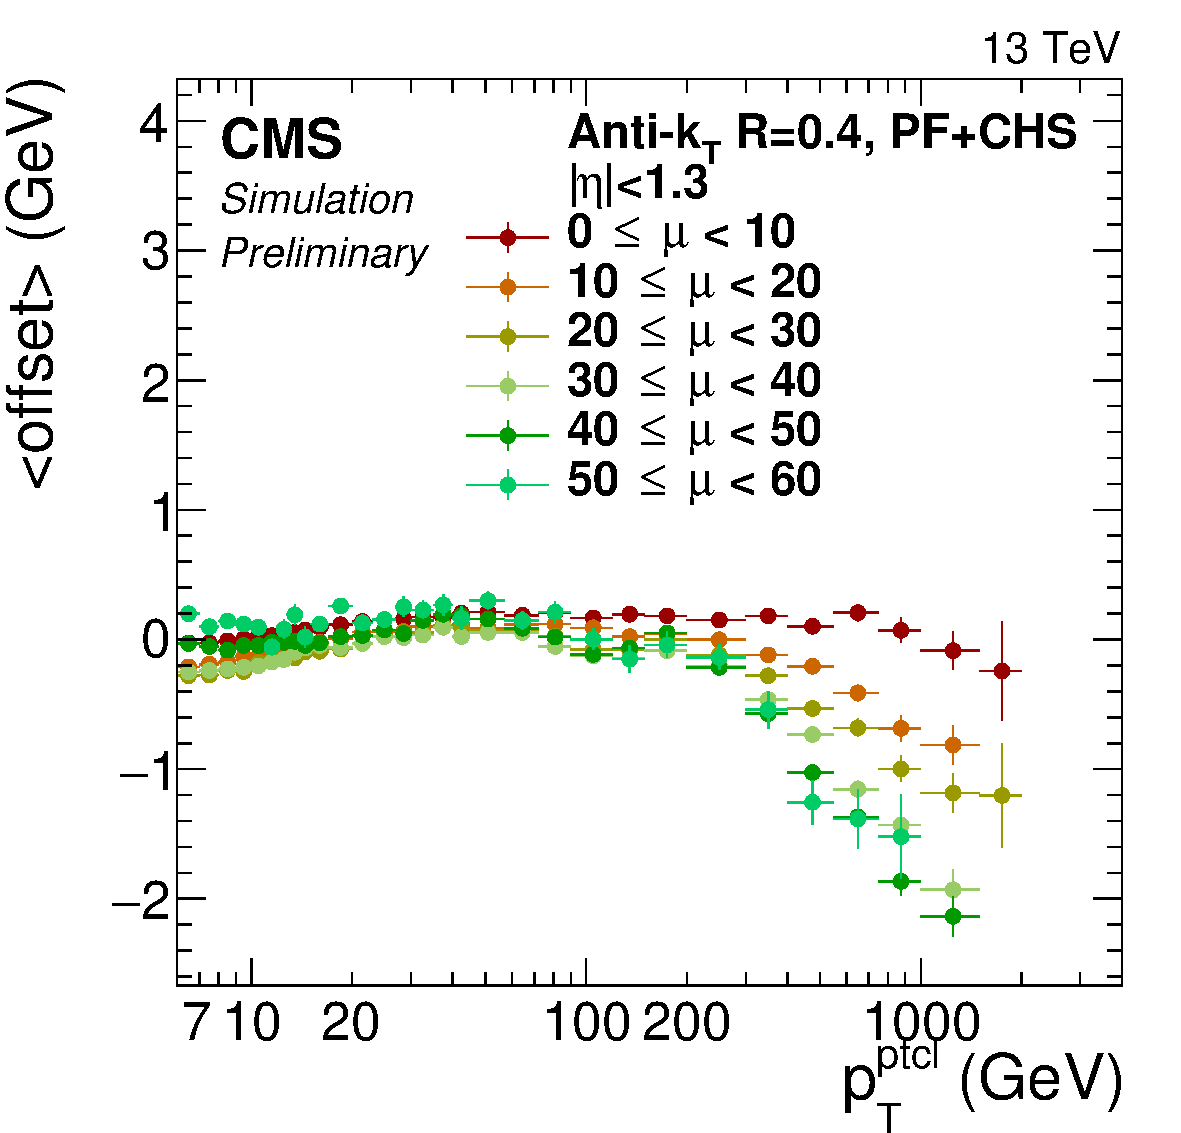
\includegraphics[width=0.5\textwidth]{images/JME-16-001/OffMeantnpuRef_BB_ak4pfchs_no2000_afterL1.pdf}
			\label{fig:OffMeantnpuRef}
		\end{figure}
	\end{textblock}
		\begin{textblock}{.9}(0.05,.25)
		\begin{figure}
			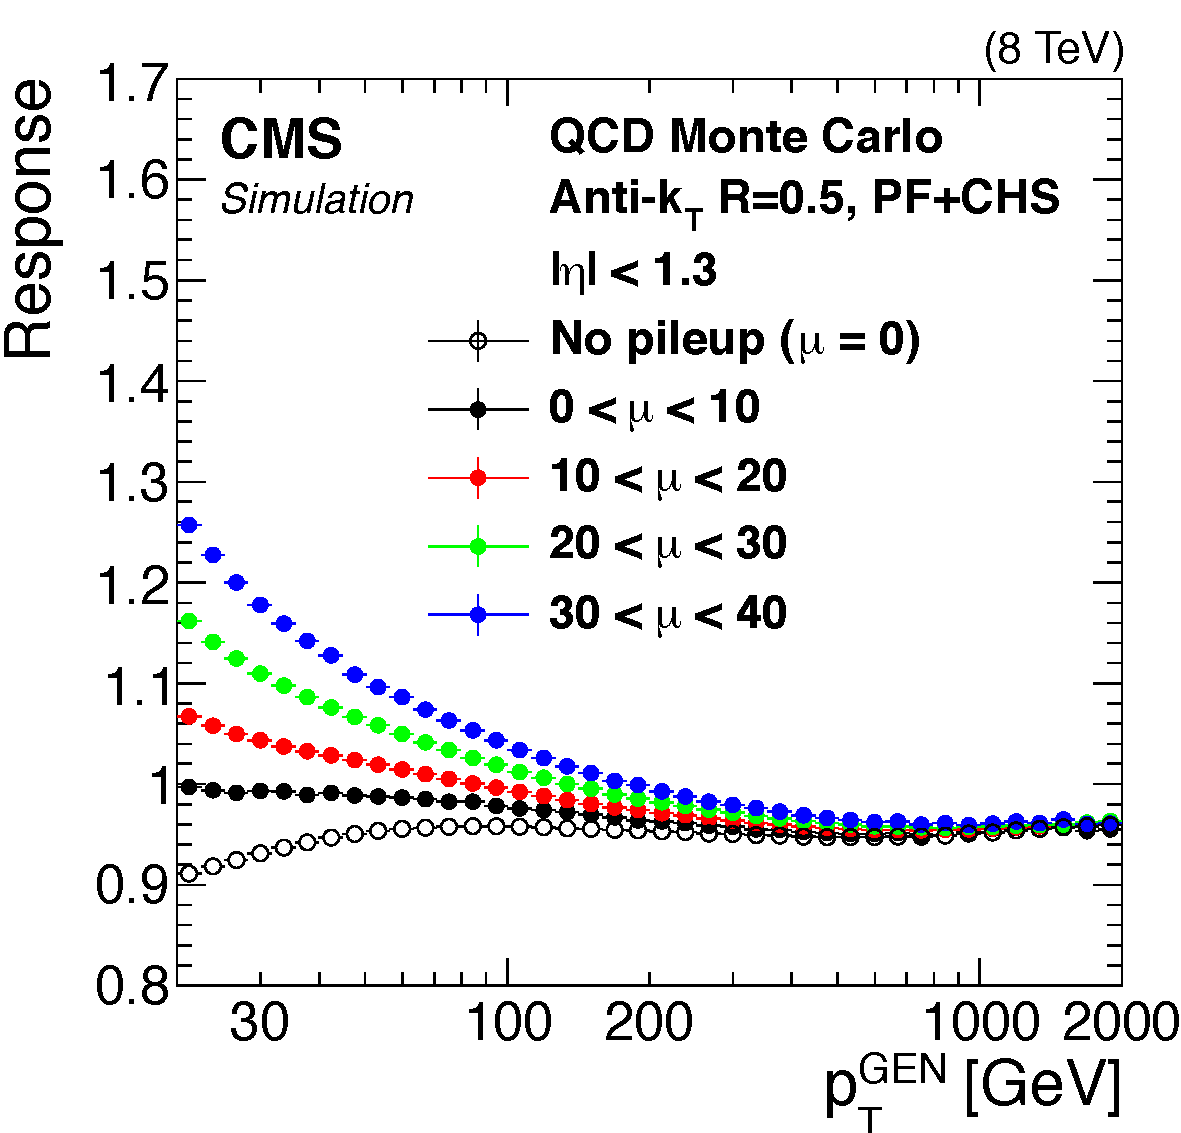
\includegraphics[width=0.5\textwidth]{images/Can0_noPreliminary.pdf} %no 13 TeV version
			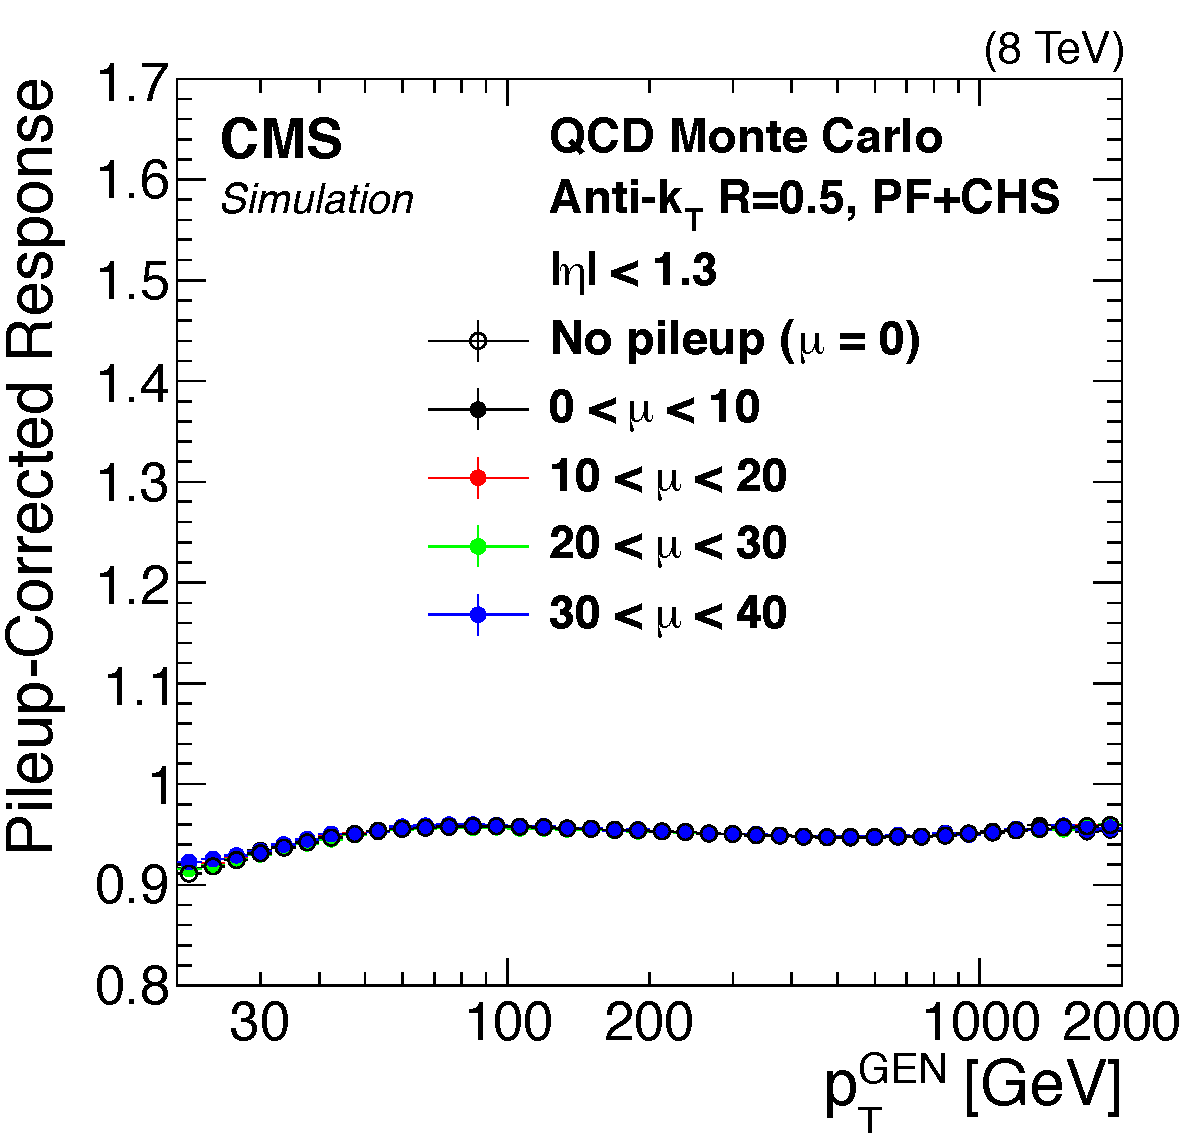
\includegraphics[width=0.5\textwidth]{images/Can1_noPreliminary.pdf} %no 13 TeV version
		\end{figure}
	\end{textblock}
}
%---------------------------------------------------------------------------------------------------------------------------------------
\frame{
	\frametitle{JECs: A Factorized Approach}
        \begin{textblock}{.9}(0.05,0.085)
		\begin{figure}
			\scalebox{.9}{
			%	\documentclass[dvipsnames]{standalone}
\usepackage{color}
\usepackage{tikz}
\usetikzlibrary{arrows,shapes,shapes.multipart,backgrounds,calc,decorations.text,decorations.pathreplacing,matrix,shadings}
\tikzstyle{every picture}+=[remember picture]
\tikzstyle{na} = [baseline=-.5ex]

\begin{document}

\tikzstyle{levels} = [rectangle, draw, text width=6em, text centered, rounded corners, minimum height=2em, midway, shading=radial,outer color=Gray,middle color=white,inner color=white, Gray]
\tikzstyle{arrow} = [draw, -latex']
\tikzstyle{line} = [draw, -]

\newcommand*{\mytextstyle}{\sffamily\Large\bfseries\color{black!85}}
\newcommand{\myarrowstart}[9]{%
% inner radius, middle radius, outer radius, start angle,
% end angle, tip protusion angle, options, text
  \pgfmathsetmacro{\start}{#1}
  \pgfmathsetmacro{\rin}{#2}
  \pgfmathsetmacro{\rmid}{#3}
  \pgfmathsetmacro{\rout}{#4}
  \pgfmathsetmacro{\astart}{#5}
  \pgfmathsetmacro{\aend}{#6}
  \pgfmathsetmacro{\atip}{#7}
  \fill[#8] (\start+\astart,\rin) -- (\start+\aend,\rin) -- (\start+\aend+\atip,\rmid)
        -- (\start+\aend,\rout) -- (\start+\astart,\rout) -- (\start+\astart,\rmid)
        -- cycle;
  \node[font = \sffamily, align=center,text width=\aend-\astart,anchor = west, yshift=-0.0ex] (arrowend) at (\start+\astart,\rmid) {\mytextstyle{#9}};
%  \path[font = \sffamily, decoration = {text along path, text = {|\mytextstyle|#9},
%    text align = {align = center}, raise = -0.5ex}, decorate]
%    (\start+\astart+0.4*\atip,\rmid) -- (\start+\aend+0.4*\atip,\rmid);
}
\newcommand{\myarrow}[9]{%
% inner radius, middle radius, outer radius, start angle,
% end angle, tip protusion angle, options, text
  \pgfmathsetmacro{\start}{#1}
  \pgfmathsetmacro{\rin}{#2}
  \pgfmathsetmacro{\rmid}{#3}
  \pgfmathsetmacro{\rout}{#4}
  \pgfmathsetmacro{\astart}{#5}
  \pgfmathsetmacro{\aend}{#6}
  \pgfmathsetmacro{\atip}{#7}
  \fill[#8] (\start+\astart,\rin) -- (\start+\aend,\rin) -- (\start+\aend+\atip,\rmid) 
        -- (\start+\aend,\rout) -- (\start+\astart,\rout) -- (\start+\astart+\atip,\rmid)
        -- cycle;
  \path[font = \sffamily, decoration = {text along path, text = {|\mytextstyle|#9},
    text align = {align = center}, raise = -0.5ex}, decorate]
    (\start+\astart+0.75*\atip,\rmid) -- (\start+\aend+0.75*\atip,\rmid);
}
\newcommand{\myuphalfarrow}[9]{%
% inner radius, middle radius, outer radius, start angle,
% end angle, tip protusion angle, options, text
  \pgfmathsetmacro{\start}{#1}
  \pgfmathsetmacro{\rin}{#2}
  \pgfmathsetmacro{\rmid}{#3}
  \pgfmathsetmacro{\rout}{#4}
  \pgfmathsetmacro{\astart}{#5}
  \pgfmathsetmacro{\aend}{#6}
  \pgfmathsetmacro{\atip}{#7}
  \fill[#8] (\start+\astart,\rout) -- (\start+\aend,\rout) -- (\start+\aend+\atip,\rin) 
        -- (\start+\astart+\atip,\rin) -- cycle;
  \path[font = \sffamily, decoration = {text along path, text = {|\mytextstyle|#9},
    text align = {align = center}, raise = -0.5ex}, decorate]
    (\start+\astart+0.4*\atip,\rmid) -- (\start+\aend+0.4*\atip,\rmid);
}
\newcommand{\mylowhalfarrow}[9]{%
% inner radius, middle radius, outer radius, start angle,
% end angle, tip protusion angle, options, text
  \pgfmathsetmacro{\start}{#1}
  \pgfmathsetmacro{\rin}{#2}
  \pgfmathsetmacro{\rmid}{#3}
  \pgfmathsetmacro{\rout}{#4}
  \pgfmathsetmacro{\astart}{#5}
  \pgfmathsetmacro{\aend}{#6}
  \pgfmathsetmacro{\atip}{#7}
  \fill[#8] (\start+\astart+\atip,\rin) -- (\start+\aend+\atip,\rin) -- (\start+\aend,\rout)
        -- (\start+\astart,\rout) -- cycle;
  \path[font = \sffamily, decoration = {text along path, text = {|\mytextstyle|#9},
    text align = {align = center}, raise = -0.5ex}, decorate]
    (\start+\astart+0.4*\atip,\rmid) -- (\start+\aend+0.4*\atip,\rmid);
}
\newcommand{\myarrowend}[9]{%
% inner radius, middle radius, outer radius, start angle,
% end angle, tip protusion angle, options, text
  \pgfmathsetmacro{\start}{#1}
  \pgfmathsetmacro{\rin}{#2}
  \pgfmathsetmacro{\rmid}{#3}
  \pgfmathsetmacro{\rout}{#4}
  \pgfmathsetmacro{\astart}{#5}
  \pgfmathsetmacro{\aend}{#6}
  \pgfmathsetmacro{\atip}{#7}
  \fill[#8] (\start+\astart,\rin) -- (\start+\aend,\rin) -- (\start+\aend,\rmid)
        -- (\start+\aend,\rout) -- (\start+\astart,\rout) -- (\start+\astart+\atip,\rmid)
        -- cycle;
  \node[font = \sffamily, align=center,text width=\aend-\astart,anchor = west, yshift=-0.0ex] (arrowend) at (\start+\astart+0.75*\atip,\rmid) {\mytextstyle{#9}};
}

\begin{tikzpicture}[node distance = 2cm, auto, scale=0.8]
\scriptsize
    % Place nodes
    \myarrowstart{0}{0.5}{1.5}{2.5}{0}{1.75}{0.5}{Cyan,draw = Cyan, very thick}{\scriptsize{Reconstructed Jets}}

    \myuphalfarrow{1.95}{1.52}{1.75}{2.5}{0}{2.0}{0.5}{Purple,draw = Purple, very thick}{|\scriptsize|{MC + RC}}
    \mylowhalfarrow{1.95}{1.48}{1.}{0.5}{0}{2.0}{0.5}{Cyan,draw = Cyan, very thick}{|\scriptsize|{MC}}

    \node [font = \sffamily, align=left,text width=2.cm,anchor = west, yshift=-0.0ex] (l1data) at (2.4,2.2) {\mytextstyle\small\color{Black}\scriptsize{Pileup}};


    \myarrow{4.15}{0.5}{1.5}{2.5}{0}{2.95}{0.5}{Red!80,draw = Red!80, very thick}{|\scriptsize|{MC}}
    \node [font = \sffamily, align=left,text width=2.cm,anchor = west, yshift=-0.0ex] (l2l3) at (4.35,2.2) {\mytextstyle\small\color{Black}\scriptsize{Response $(p_{T},\eta)$ }};


    \myuphalfarrow{7.3}{1.52}{1.75}{2.5}{0}{1.9}{0.5}{BurntOrange,draw = BurntOrange, very thick}{|\scriptsize|{dijets}}
    \node [font = \sffamily, align=left,text width=2.cm,anchor = west, yshift=-0.0ex] (l2res) at (7.4,2.2) {\mytextstyle\small\color{Black}\scriptsize{Residuals$(\eta)$}};
    \mylowhalfarrow{7.3}{1.48}{1.25}{0.5}{0}{1.9}{0.5}{yellow!20,draw = yellow!20, very thick}{}


   \myuphalfarrow{9.4}{1.52}{1.75}{2.5}{0}{2.4}{0.5}{BurntOrange,draw = BurntOrange, very thick}{|\scriptsize|{   $\gamma$/Z$+$jet, MJB}}
    \node [font = \sffamily, align=left,text width=2.cm,anchor = west, yshift=-0.0ex] (l3res) at (9.6,2.2) {\mytextstyle\small\color{Black}\scriptsize{Residuals$(p_T)$}};
    \mylowhalfarrow{9.4}{1.48}{1.25}{0.5}{0}{2.4}{0.5}{yellow!20,draw = yellow!20, very thick}{}

 
   \myarrow{12.0}{0.5}{1.5}{2.5}{0}{1.}{0.5}{Yellow!80,draw = Yellow!80, very thick}{|\scriptsize|{MC}}
    \node [font = \sffamily, align=left,text width=2.cm,anchor = west, yshift=-0.0ex] (l5) at (12.,2.2) {\mytextstyle\small\color{Black}\scriptsize{ Flavor}};


    \myarrowend{13.20}{0.5}{1.5}{2.5}{0}{2.}{0.5}{Green!90,draw = Green!90, very thick}{\scriptsize{Calibrated Jets}}
    
    \node [font = \sffamily, align=left,text width=2.75cm,anchor = west, yshift=-0.0ex] (MC) at (2.25,0.) {\mytextstyle\small\color{RoyalBlue}Applied on MC};
    \node [font = \sffamily, align=left,text width=2.75cm,anchor = west, yshift=-0.0ex] (DATA) at (2.25,3.) {\mytextstyle\small\color{YellowOrange}Applied on data};

    \node [font = \sffamily, align=left,text width=5cm,anchor = west, yshift=-0.0ex] (INSITU) at (7.6,3.) %%{\mytextstyle\footnotesize{From in-situ MPF/Z-jet, flat in $p_{T}$}};
   {\mytextstyle\footnotesize{}};
    \node [font = \sffamily, align=left,text width=5cm,anchor = west, yshift=-0.0ex] (STARTBRACE) at (7.6,0.) {};
    \node [font = \sffamily, align=left,text width=5cm,anchor = west, yshift=-0.0ex] (ENDBRACE) at (12.65,0.5) {};
    \path[arrow,YellowOrange,thick, shorten <= -0.5cm] (DATA) -- (INSITU);
%    \draw [thick, decorate, decoration = {brace, amplitude = 10pt, mirror}, xshift = 0pt, yshift = 0pt] (7.25,0.75) -- (12.0,0.75) node [black, midway, xshift = 0cm, yshift = -0.8cm] {\mytextstyle\small{stuff}};
 %   \draw [thick, decorate, decoration = {brace, amplitude = 10pt, mirror}, xshift = 0pt, yshift = 0pt] (7.7,0.75) -- (12.65,0.75) node [levels, xshift = 0cm, yshift = -1.0cm] {\mytextstyle\scriptsize{L2L3Res}};

   \path[arrow,RoyalBlue,thick, shorten <= -0.5cm] (MC) -- (STARTBRACE);

 %   \node [levels, below of=MC, xshift = 3.6cm, yshift = 1.85cm, thick] (L1) {\mytextstyle\small{L1}};
 %   \node [levels, right of=L1, xshift = 4.4cm, yshift = -0.15cm, thick] (L2L3) {\mytextstyle\small{L2L3}};
\end{tikzpicture}

\end{document}

				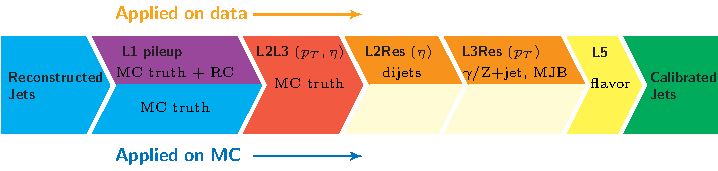
\includegraphics[width=\textwidth]{images/CMS_JEC_levels.pdf}
			}
			\label{fig:factorized_approach}
		\end{figure}
	\end{textblock}
	\vspace*{2.4cm}
	\begin{block}{MC-truth $\eta$ \& $p_{T}$ Corrections}
		\begin{itemize}
			\footnotesize
			\item L2Relative \& L3Absolute corrections seek to make the jet response flat vs $p_{T}$ and $\eta$
			\item During this step jets are corrected back to particle level so that the corrected jet $p_{T}$ is equal, on average, to the GenJet $p_{T}$
			\item Every effort is taken to make these corrections independent of the jet $p_{T}$ spectrum
			\item Derived on a QCD sample, but must be applicable to all physics processes
		\end{itemize}			
	\end{block}
	\vspace*{-0.15cm}
	\begin{alertblock}{Bombshell \#1}
		\footnotesize
		\begin{itemize}
			\item The L2Relative \& L3Absolute corrections are derived in one step
			\item They used to be separate, but we have combined them into one set of constants contained in the L2Relative payload
			\item The L3Absolute payload now contains a multiplicative factor of one, but is still there for future use
		\end{itemize}
	\end{alertblock}
}
%---------------------------------------------------------------------------------------------------------------------------------------
\frame{
	\frametitle{JECs: A Factorized Approach}
        \begin{textblock}{.9}(0.05,0.085)
		\begin{figure}
			\scalebox{.9}{
			%	\documentclass[dvipsnames]{standalone}
\usepackage{color}
\usepackage{tikz}
\usetikzlibrary{arrows,shapes,shapes.multipart,backgrounds,calc,decorations.text,decorations.pathreplacing,matrix,shadings}
\tikzstyle{every picture}+=[remember picture]
\tikzstyle{na} = [baseline=-.5ex]

\begin{document}

\tikzstyle{levels} = [rectangle, draw, text width=6em, text centered, rounded corners, minimum height=2em, midway, shading=radial,outer color=Gray,middle color=white,inner color=white, Gray]
\tikzstyle{arrow} = [draw, -latex']
\tikzstyle{line} = [draw, -]

\newcommand*{\mytextstyle}{\sffamily\Large\bfseries\color{black!85}}
\newcommand{\myarrowstart}[9]{%
% inner radius, middle radius, outer radius, start angle,
% end angle, tip protusion angle, options, text
  \pgfmathsetmacro{\start}{#1}
  \pgfmathsetmacro{\rin}{#2}
  \pgfmathsetmacro{\rmid}{#3}
  \pgfmathsetmacro{\rout}{#4}
  \pgfmathsetmacro{\astart}{#5}
  \pgfmathsetmacro{\aend}{#6}
  \pgfmathsetmacro{\atip}{#7}
  \fill[#8] (\start+\astart,\rin) -- (\start+\aend,\rin) -- (\start+\aend+\atip,\rmid)
        -- (\start+\aend,\rout) -- (\start+\astart,\rout) -- (\start+\astart,\rmid)
        -- cycle;
  \node[font = \sffamily, align=center,text width=\aend-\astart,anchor = west, yshift=-0.0ex] (arrowend) at (\start+\astart,\rmid) {\mytextstyle{#9}};
%  \path[font = \sffamily, decoration = {text along path, text = {|\mytextstyle|#9},
%    text align = {align = center}, raise = -0.5ex}, decorate]
%    (\start+\astart+0.4*\atip,\rmid) -- (\start+\aend+0.4*\atip,\rmid);
}
\newcommand{\myarrow}[9]{%
% inner radius, middle radius, outer radius, start angle,
% end angle, tip protusion angle, options, text
  \pgfmathsetmacro{\start}{#1}
  \pgfmathsetmacro{\rin}{#2}
  \pgfmathsetmacro{\rmid}{#3}
  \pgfmathsetmacro{\rout}{#4}
  \pgfmathsetmacro{\astart}{#5}
  \pgfmathsetmacro{\aend}{#6}
  \pgfmathsetmacro{\atip}{#7}
  \fill[#8] (\start+\astart,\rin) -- (\start+\aend,\rin) -- (\start+\aend+\atip,\rmid) 
        -- (\start+\aend,\rout) -- (\start+\astart,\rout) -- (\start+\astart+\atip,\rmid)
        -- cycle;
  \path[font = \sffamily, decoration = {text along path, text = {|\mytextstyle|#9},
    text align = {align = center}, raise = -0.5ex}, decorate]
    (\start+\astart+0.75*\atip,\rmid) -- (\start+\aend+0.75*\atip,\rmid);
}
\newcommand{\myuphalfarrow}[9]{%
% inner radius, middle radius, outer radius, start angle,
% end angle, tip protusion angle, options, text
  \pgfmathsetmacro{\start}{#1}
  \pgfmathsetmacro{\rin}{#2}
  \pgfmathsetmacro{\rmid}{#3}
  \pgfmathsetmacro{\rout}{#4}
  \pgfmathsetmacro{\astart}{#5}
  \pgfmathsetmacro{\aend}{#6}
  \pgfmathsetmacro{\atip}{#7}
  \fill[#8] (\start+\astart,\rout) -- (\start+\aend,\rout) -- (\start+\aend+\atip,\rin) 
        -- (\start+\astart+\atip,\rin) -- cycle;
  \path[font = \sffamily, decoration = {text along path, text = {|\mytextstyle|#9},
    text align = {align = center}, raise = -0.5ex}, decorate]
    (\start+\astart+0.4*\atip,\rmid) -- (\start+\aend+0.4*\atip,\rmid);
}
\newcommand{\mylowhalfarrow}[9]{%
% inner radius, middle radius, outer radius, start angle,
% end angle, tip protusion angle, options, text
  \pgfmathsetmacro{\start}{#1}
  \pgfmathsetmacro{\rin}{#2}
  \pgfmathsetmacro{\rmid}{#3}
  \pgfmathsetmacro{\rout}{#4}
  \pgfmathsetmacro{\astart}{#5}
  \pgfmathsetmacro{\aend}{#6}
  \pgfmathsetmacro{\atip}{#7}
  \fill[#8] (\start+\astart+\atip,\rin) -- (\start+\aend+\atip,\rin) -- (\start+\aend,\rout)
        -- (\start+\astart,\rout) -- cycle;
  \path[font = \sffamily, decoration = {text along path, text = {|\mytextstyle|#9},
    text align = {align = center}, raise = -0.5ex}, decorate]
    (\start+\astart+0.4*\atip,\rmid) -- (\start+\aend+0.4*\atip,\rmid);
}
\newcommand{\myarrowend}[9]{%
% inner radius, middle radius, outer radius, start angle,
% end angle, tip protusion angle, options, text
  \pgfmathsetmacro{\start}{#1}
  \pgfmathsetmacro{\rin}{#2}
  \pgfmathsetmacro{\rmid}{#3}
  \pgfmathsetmacro{\rout}{#4}
  \pgfmathsetmacro{\astart}{#5}
  \pgfmathsetmacro{\aend}{#6}
  \pgfmathsetmacro{\atip}{#7}
  \fill[#8] (\start+\astart,\rin) -- (\start+\aend,\rin) -- (\start+\aend,\rmid)
        -- (\start+\aend,\rout) -- (\start+\astart,\rout) -- (\start+\astart+\atip,\rmid)
        -- cycle;
  \node[font = \sffamily, align=center,text width=\aend-\astart,anchor = west, yshift=-0.0ex] (arrowend) at (\start+\astart+0.75*\atip,\rmid) {\mytextstyle{#9}};
}

\begin{tikzpicture}[node distance = 2cm, auto, scale=0.8]
\scriptsize
    % Place nodes
    \myarrowstart{0}{0.5}{1.5}{2.5}{0}{1.75}{0.5}{Cyan,draw = Cyan, very thick}{\scriptsize{Reconstructed Jets}}

    \myuphalfarrow{1.95}{1.52}{1.75}{2.5}{0}{2.0}{0.5}{Purple,draw = Purple, very thick}{|\scriptsize|{MC + RC}}
    \mylowhalfarrow{1.95}{1.48}{1.}{0.5}{0}{2.0}{0.5}{Cyan,draw = Cyan, very thick}{|\scriptsize|{MC}}

    \node [font = \sffamily, align=left,text width=2.cm,anchor = west, yshift=-0.0ex] (l1data) at (2.4,2.2) {\mytextstyle\small\color{Black}\scriptsize{Pileup}};


    \myarrow{4.15}{0.5}{1.5}{2.5}{0}{2.95}{0.5}{Red!80,draw = Red!80, very thick}{|\scriptsize|{MC}}
    \node [font = \sffamily, align=left,text width=2.cm,anchor = west, yshift=-0.0ex] (l2l3) at (4.35,2.2) {\mytextstyle\small\color{Black}\scriptsize{Response $(p_{T},\eta)$ }};


    \myuphalfarrow{7.3}{1.52}{1.75}{2.5}{0}{1.9}{0.5}{BurntOrange,draw = BurntOrange, very thick}{|\scriptsize|{dijets}}
    \node [font = \sffamily, align=left,text width=2.cm,anchor = west, yshift=-0.0ex] (l2res) at (7.4,2.2) {\mytextstyle\small\color{Black}\scriptsize{Residuals$(\eta)$}};
    \mylowhalfarrow{7.3}{1.48}{1.25}{0.5}{0}{1.9}{0.5}{yellow!20,draw = yellow!20, very thick}{}


   \myuphalfarrow{9.4}{1.52}{1.75}{2.5}{0}{2.4}{0.5}{BurntOrange,draw = BurntOrange, very thick}{|\scriptsize|{   $\gamma$/Z$+$jet, MJB}}
    \node [font = \sffamily, align=left,text width=2.cm,anchor = west, yshift=-0.0ex] (l3res) at (9.6,2.2) {\mytextstyle\small\color{Black}\scriptsize{Residuals$(p_T)$}};
    \mylowhalfarrow{9.4}{1.48}{1.25}{0.5}{0}{2.4}{0.5}{yellow!20,draw = yellow!20, very thick}{}

 
   \myarrow{12.0}{0.5}{1.5}{2.5}{0}{1.}{0.5}{Yellow!80,draw = Yellow!80, very thick}{|\scriptsize|{MC}}
    \node [font = \sffamily, align=left,text width=2.cm,anchor = west, yshift=-0.0ex] (l5) at (12.,2.2) {\mytextstyle\small\color{Black}\scriptsize{ Flavor}};


    \myarrowend{13.20}{0.5}{1.5}{2.5}{0}{2.}{0.5}{Green!90,draw = Green!90, very thick}{\scriptsize{Calibrated Jets}}
    
    \node [font = \sffamily, align=left,text width=2.75cm,anchor = west, yshift=-0.0ex] (MC) at (2.25,0.) {\mytextstyle\small\color{RoyalBlue}Applied on MC};
    \node [font = \sffamily, align=left,text width=2.75cm,anchor = west, yshift=-0.0ex] (DATA) at (2.25,3.) {\mytextstyle\small\color{YellowOrange}Applied on data};

    \node [font = \sffamily, align=left,text width=5cm,anchor = west, yshift=-0.0ex] (INSITU) at (7.6,3.) %%{\mytextstyle\footnotesize{From in-situ MPF/Z-jet, flat in $p_{T}$}};
   {\mytextstyle\footnotesize{}};
    \node [font = \sffamily, align=left,text width=5cm,anchor = west, yshift=-0.0ex] (STARTBRACE) at (7.6,0.) {};
    \node [font = \sffamily, align=left,text width=5cm,anchor = west, yshift=-0.0ex] (ENDBRACE) at (12.65,0.5) {};
    \path[arrow,YellowOrange,thick, shorten <= -0.5cm] (DATA) -- (INSITU);
%    \draw [thick, decorate, decoration = {brace, amplitude = 10pt, mirror}, xshift = 0pt, yshift = 0pt] (7.25,0.75) -- (12.0,0.75) node [black, midway, xshift = 0cm, yshift = -0.8cm] {\mytextstyle\small{stuff}};
 %   \draw [thick, decorate, decoration = {brace, amplitude = 10pt, mirror}, xshift = 0pt, yshift = 0pt] (7.7,0.75) -- (12.65,0.75) node [levels, xshift = 0cm, yshift = -1.0cm] {\mytextstyle\scriptsize{L2L3Res}};

   \path[arrow,RoyalBlue,thick, shorten <= -0.5cm] (MC) -- (STARTBRACE);

 %   \node [levels, below of=MC, xshift = 3.6cm, yshift = 1.85cm, thick] (L1) {\mytextstyle\small{L1}};
 %   \node [levels, right of=L1, xshift = 4.4cm, yshift = -0.15cm, thick] (L2L3) {\mytextstyle\small{L2L3}};
\end{tikzpicture}

\end{document}

				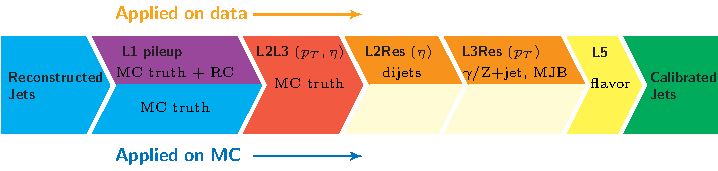
\includegraphics[width=\textwidth]{images/CMS_JEC_levels.pdf}
			}
			\label{fig:factorized_approach}
		\end{figure}
	\end{textblock}
	\vspace*{2.4cm}
	\begin{block}{MC-truth $\eta$ \& $p_{T}$ Corrections}
		\begin{itemize}
			\footnotesize
			\item L2Relative \& L3Absolute corrections seek to make the jet response flat vs $p_{T}$ and $\eta$
			\item During this step jets are corrected back to particle level so that the corrected jet $p_{T}$ is equal, on average, to the GenJet $p_{T}$
			\item Every effort is taken to make these corrections independent of the jet $p_{T}$ spectrum
			\item Derived on a QCD sample, but must be applicable to all physics processes
		\end{itemize}			
	\end{block}
	\vspace*{-0.15cm}
	\begin{alertblock}{Bombshell \#1}
		\footnotesize
		\begin{itemize}
			\item The L2Relative \& L3Absolute corrections are derived in one step
			\item They used to be separate, but we have combined them into one set of constants contained in the L2Relative payload
			\item The L3Absolute payload now contains a multiplicative factor of one, but is still there for future use
		\end{itemize}
	\end{alertblock}
	
	\begin{textblock}{.9}(0.05,.25)
		\begin{figure}
			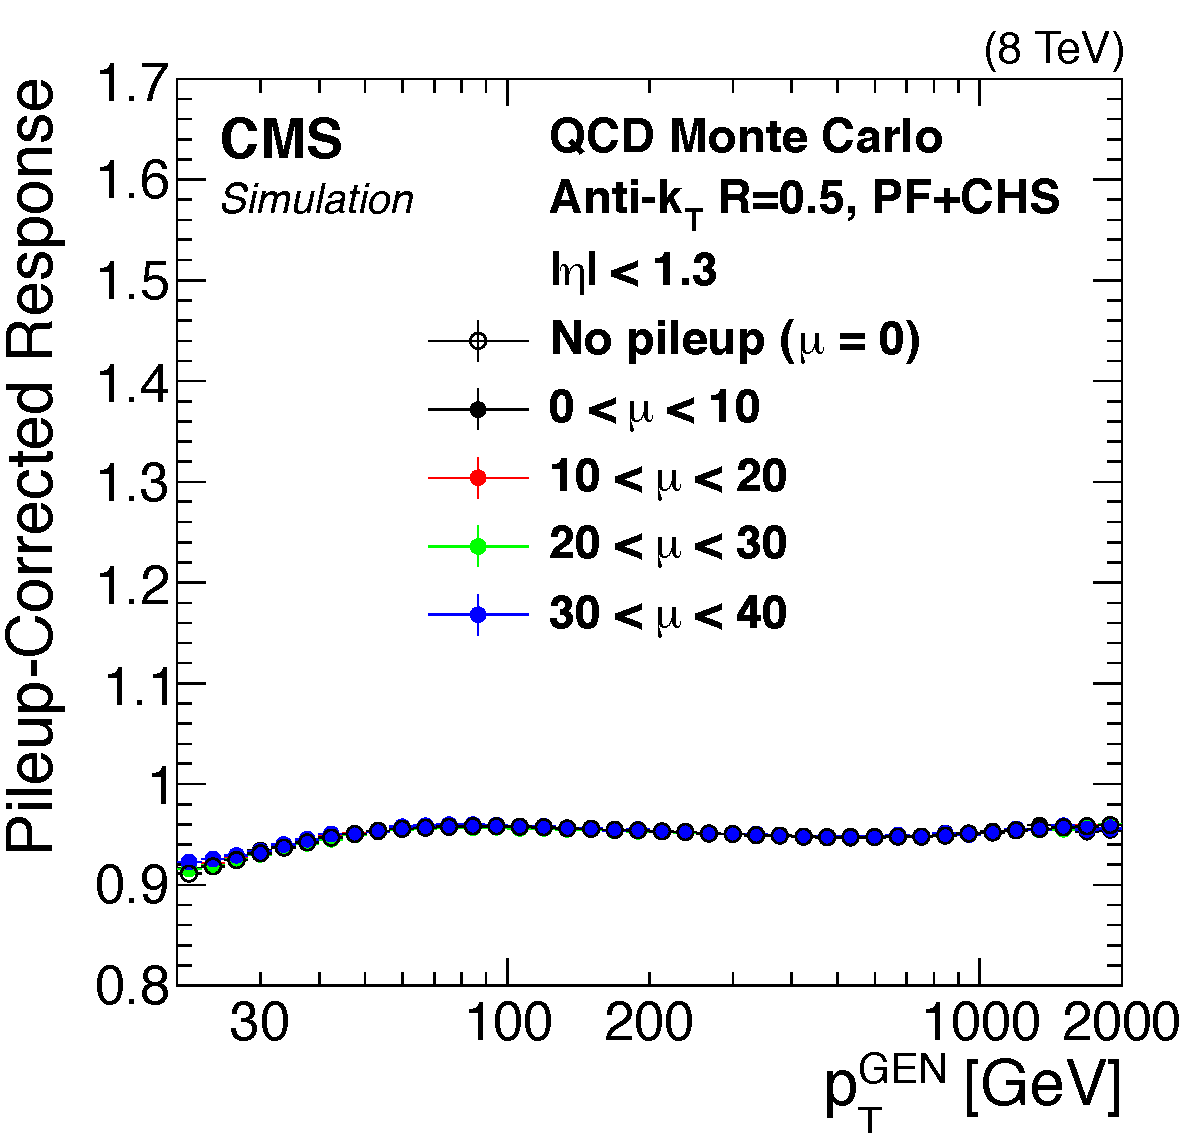
\includegraphics[width=0.5\textwidth]{images/Can1_noPreliminary.pdf}  %no 13 TeV version
			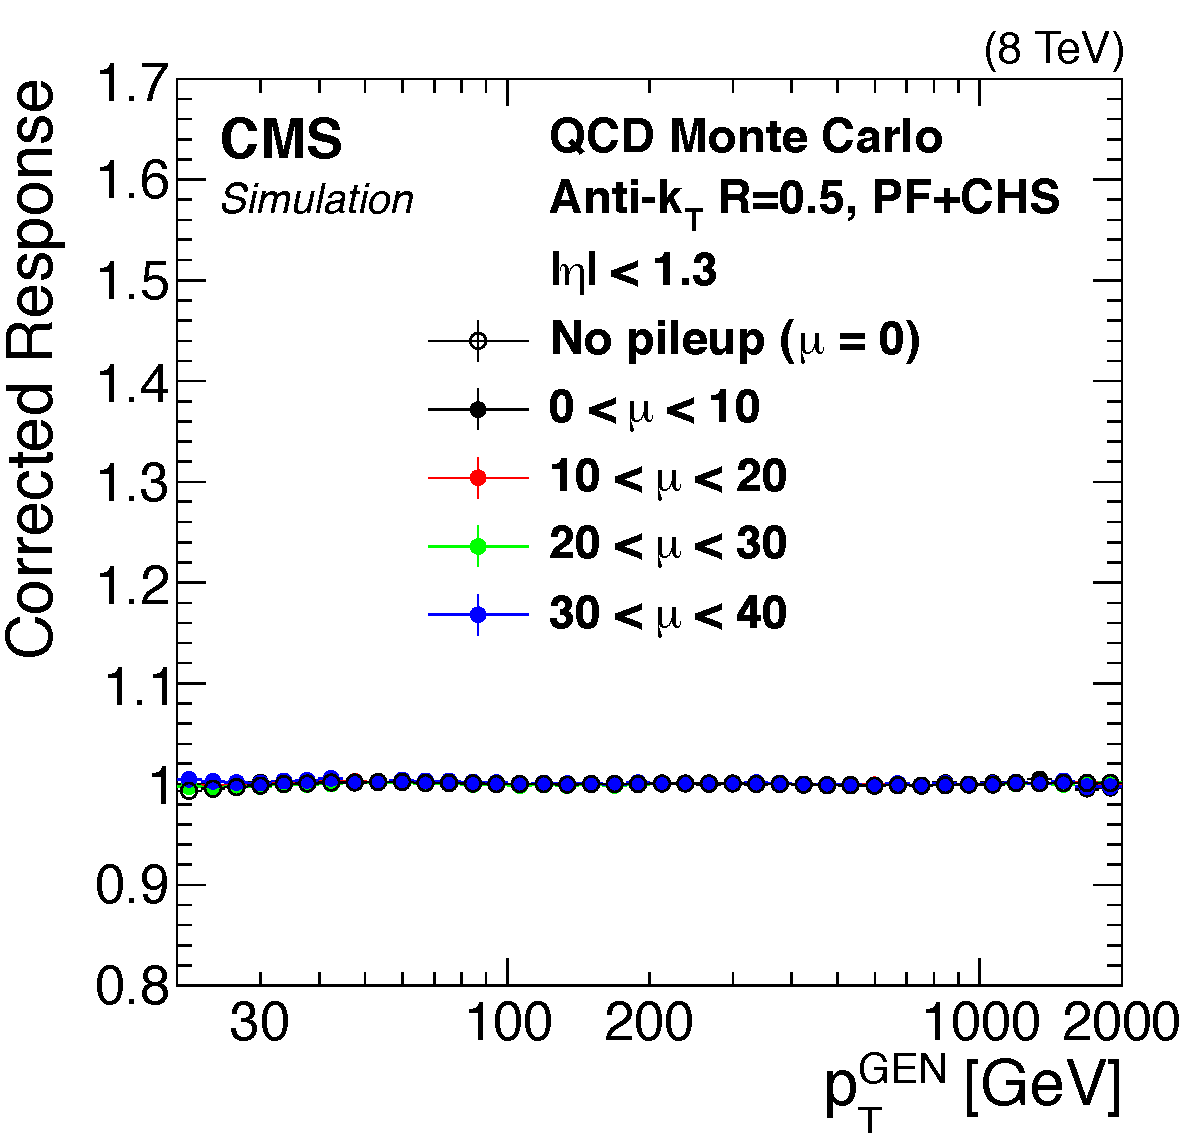
\includegraphics[width=0.5\textwidth]{images/Can2_noPreliminary.pdf}  %no 13 TeV version
			\label{fig:closurel1l2l3}
		\end{figure}
	\end{textblock}
}
%---------------------------------------------------------------------------------------------------------------------------------------
\frame{
	\frametitle{JECs: A Factorized Approach}
        \begin{textblock}{.9}(0.05,0.085)
		\begin{figure}
			\scalebox{.9}{
			%	\documentclass[dvipsnames]{standalone}
\usepackage{color}
\usepackage{tikz}
\usetikzlibrary{arrows,shapes,shapes.multipart,backgrounds,calc,decorations.text,decorations.pathreplacing,matrix,shadings}
\tikzstyle{every picture}+=[remember picture]
\tikzstyle{na} = [baseline=-.5ex]

\begin{document}

\tikzstyle{levels} = [rectangle, draw, text width=6em, text centered, rounded corners, minimum height=2em, midway, shading=radial,outer color=Gray,middle color=white,inner color=white, Gray]
\tikzstyle{arrow} = [draw, -latex']
\tikzstyle{line} = [draw, -]

\newcommand*{\mytextstyle}{\sffamily\Large\bfseries\color{black!85}}
\newcommand{\myarrowstart}[9]{%
% inner radius, middle radius, outer radius, start angle,
% end angle, tip protusion angle, options, text
  \pgfmathsetmacro{\start}{#1}
  \pgfmathsetmacro{\rin}{#2}
  \pgfmathsetmacro{\rmid}{#3}
  \pgfmathsetmacro{\rout}{#4}
  \pgfmathsetmacro{\astart}{#5}
  \pgfmathsetmacro{\aend}{#6}
  \pgfmathsetmacro{\atip}{#7}
  \fill[#8] (\start+\astart,\rin) -- (\start+\aend,\rin) -- (\start+\aend+\atip,\rmid)
        -- (\start+\aend,\rout) -- (\start+\astart,\rout) -- (\start+\astart,\rmid)
        -- cycle;
  \node[font = \sffamily, align=center,text width=\aend-\astart,anchor = west, yshift=-0.0ex] (arrowend) at (\start+\astart,\rmid) {\mytextstyle{#9}};
%  \path[font = \sffamily, decoration = {text along path, text = {|\mytextstyle|#9},
%    text align = {align = center}, raise = -0.5ex}, decorate]
%    (\start+\astart+0.4*\atip,\rmid) -- (\start+\aend+0.4*\atip,\rmid);
}
\newcommand{\myarrow}[9]{%
% inner radius, middle radius, outer radius, start angle,
% end angle, tip protusion angle, options, text
  \pgfmathsetmacro{\start}{#1}
  \pgfmathsetmacro{\rin}{#2}
  \pgfmathsetmacro{\rmid}{#3}
  \pgfmathsetmacro{\rout}{#4}
  \pgfmathsetmacro{\astart}{#5}
  \pgfmathsetmacro{\aend}{#6}
  \pgfmathsetmacro{\atip}{#7}
  \fill[#8] (\start+\astart,\rin) -- (\start+\aend,\rin) -- (\start+\aend+\atip,\rmid) 
        -- (\start+\aend,\rout) -- (\start+\astart,\rout) -- (\start+\astart+\atip,\rmid)
        -- cycle;
  \path[font = \sffamily, decoration = {text along path, text = {|\mytextstyle|#9},
    text align = {align = center}, raise = -0.5ex}, decorate]
    (\start+\astart+0.75*\atip,\rmid) -- (\start+\aend+0.75*\atip,\rmid);
}
\newcommand{\myuphalfarrow}[9]{%
% inner radius, middle radius, outer radius, start angle,
% end angle, tip protusion angle, options, text
  \pgfmathsetmacro{\start}{#1}
  \pgfmathsetmacro{\rin}{#2}
  \pgfmathsetmacro{\rmid}{#3}
  \pgfmathsetmacro{\rout}{#4}
  \pgfmathsetmacro{\astart}{#5}
  \pgfmathsetmacro{\aend}{#6}
  \pgfmathsetmacro{\atip}{#7}
  \fill[#8] (\start+\astart,\rout) -- (\start+\aend,\rout) -- (\start+\aend+\atip,\rin) 
        -- (\start+\astart+\atip,\rin) -- cycle;
  \path[font = \sffamily, decoration = {text along path, text = {|\mytextstyle|#9},
    text align = {align = center}, raise = -0.5ex}, decorate]
    (\start+\astart+0.4*\atip,\rmid) -- (\start+\aend+0.4*\atip,\rmid);
}
\newcommand{\mylowhalfarrow}[9]{%
% inner radius, middle radius, outer radius, start angle,
% end angle, tip protusion angle, options, text
  \pgfmathsetmacro{\start}{#1}
  \pgfmathsetmacro{\rin}{#2}
  \pgfmathsetmacro{\rmid}{#3}
  \pgfmathsetmacro{\rout}{#4}
  \pgfmathsetmacro{\astart}{#5}
  \pgfmathsetmacro{\aend}{#6}
  \pgfmathsetmacro{\atip}{#7}
  \fill[#8] (\start+\astart+\atip,\rin) -- (\start+\aend+\atip,\rin) -- (\start+\aend,\rout)
        -- (\start+\astart,\rout) -- cycle;
  \path[font = \sffamily, decoration = {text along path, text = {|\mytextstyle|#9},
    text align = {align = center}, raise = -0.5ex}, decorate]
    (\start+\astart+0.4*\atip,\rmid) -- (\start+\aend+0.4*\atip,\rmid);
}
\newcommand{\myarrowend}[9]{%
% inner radius, middle radius, outer radius, start angle,
% end angle, tip protusion angle, options, text
  \pgfmathsetmacro{\start}{#1}
  \pgfmathsetmacro{\rin}{#2}
  \pgfmathsetmacro{\rmid}{#3}
  \pgfmathsetmacro{\rout}{#4}
  \pgfmathsetmacro{\astart}{#5}
  \pgfmathsetmacro{\aend}{#6}
  \pgfmathsetmacro{\atip}{#7}
  \fill[#8] (\start+\astart,\rin) -- (\start+\aend,\rin) -- (\start+\aend,\rmid)
        -- (\start+\aend,\rout) -- (\start+\astart,\rout) -- (\start+\astart+\atip,\rmid)
        -- cycle;
  \node[font = \sffamily, align=center,text width=\aend-\astart,anchor = west, yshift=-0.0ex] (arrowend) at (\start+\astart+0.75*\atip,\rmid) {\mytextstyle{#9}};
}

\begin{tikzpicture}[node distance = 2cm, auto, scale=0.8]
\scriptsize
    % Place nodes
    \myarrowstart{0}{0.5}{1.5}{2.5}{0}{1.75}{0.5}{Cyan,draw = Cyan, very thick}{\scriptsize{Reconstructed Jets}}

    \myuphalfarrow{1.95}{1.52}{1.75}{2.5}{0}{2.0}{0.5}{Purple,draw = Purple, very thick}{|\scriptsize|{MC + RC}}
    \mylowhalfarrow{1.95}{1.48}{1.}{0.5}{0}{2.0}{0.5}{Cyan,draw = Cyan, very thick}{|\scriptsize|{MC}}

    \node [font = \sffamily, align=left,text width=2.cm,anchor = west, yshift=-0.0ex] (l1data) at (2.4,2.2) {\mytextstyle\small\color{Black}\scriptsize{Pileup}};


    \myarrow{4.15}{0.5}{1.5}{2.5}{0}{2.95}{0.5}{Red!80,draw = Red!80, very thick}{|\scriptsize|{MC}}
    \node [font = \sffamily, align=left,text width=2.cm,anchor = west, yshift=-0.0ex] (l2l3) at (4.35,2.2) {\mytextstyle\small\color{Black}\scriptsize{Response $(p_{T},\eta)$ }};


    \myuphalfarrow{7.3}{1.52}{1.75}{2.5}{0}{1.9}{0.5}{BurntOrange,draw = BurntOrange, very thick}{|\scriptsize|{dijets}}
    \node [font = \sffamily, align=left,text width=2.cm,anchor = west, yshift=-0.0ex] (l2res) at (7.4,2.2) {\mytextstyle\small\color{Black}\scriptsize{Residuals$(\eta)$}};
    \mylowhalfarrow{7.3}{1.48}{1.25}{0.5}{0}{1.9}{0.5}{yellow!20,draw = yellow!20, very thick}{}


   \myuphalfarrow{9.4}{1.52}{1.75}{2.5}{0}{2.4}{0.5}{BurntOrange,draw = BurntOrange, very thick}{|\scriptsize|{   $\gamma$/Z$+$jet, MJB}}
    \node [font = \sffamily, align=left,text width=2.cm,anchor = west, yshift=-0.0ex] (l3res) at (9.6,2.2) {\mytextstyle\small\color{Black}\scriptsize{Residuals$(p_T)$}};
    \mylowhalfarrow{9.4}{1.48}{1.25}{0.5}{0}{2.4}{0.5}{yellow!20,draw = yellow!20, very thick}{}

 
   \myarrow{12.0}{0.5}{1.5}{2.5}{0}{1.}{0.5}{Yellow!80,draw = Yellow!80, very thick}{|\scriptsize|{MC}}
    \node [font = \sffamily, align=left,text width=2.cm,anchor = west, yshift=-0.0ex] (l5) at (12.,2.2) {\mytextstyle\small\color{Black}\scriptsize{ Flavor}};


    \myarrowend{13.20}{0.5}{1.5}{2.5}{0}{2.}{0.5}{Green!90,draw = Green!90, very thick}{\scriptsize{Calibrated Jets}}
    
    \node [font = \sffamily, align=left,text width=2.75cm,anchor = west, yshift=-0.0ex] (MC) at (2.25,0.) {\mytextstyle\small\color{RoyalBlue}Applied on MC};
    \node [font = \sffamily, align=left,text width=2.75cm,anchor = west, yshift=-0.0ex] (DATA) at (2.25,3.) {\mytextstyle\small\color{YellowOrange}Applied on data};

    \node [font = \sffamily, align=left,text width=5cm,anchor = west, yshift=-0.0ex] (INSITU) at (7.6,3.) %%{\mytextstyle\footnotesize{From in-situ MPF/Z-jet, flat in $p_{T}$}};
   {\mytextstyle\footnotesize{}};
    \node [font = \sffamily, align=left,text width=5cm,anchor = west, yshift=-0.0ex] (STARTBRACE) at (7.6,0.) {};
    \node [font = \sffamily, align=left,text width=5cm,anchor = west, yshift=-0.0ex] (ENDBRACE) at (12.65,0.5) {};
    \path[arrow,YellowOrange,thick, shorten <= -0.5cm] (DATA) -- (INSITU);
%    \draw [thick, decorate, decoration = {brace, amplitude = 10pt, mirror}, xshift = 0pt, yshift = 0pt] (7.25,0.75) -- (12.0,0.75) node [black, midway, xshift = 0cm, yshift = -0.8cm] {\mytextstyle\small{stuff}};
 %   \draw [thick, decorate, decoration = {brace, amplitude = 10pt, mirror}, xshift = 0pt, yshift = 0pt] (7.7,0.75) -- (12.65,0.75) node [levels, xshift = 0cm, yshift = -1.0cm] {\mytextstyle\scriptsize{L2L3Res}};

   \path[arrow,RoyalBlue,thick, shorten <= -0.5cm] (MC) -- (STARTBRACE);

 %   \node [levels, below of=MC, xshift = 3.6cm, yshift = 1.85cm, thick] (L1) {\mytextstyle\small{L1}};
 %   \node [levels, right of=L1, xshift = 4.4cm, yshift = -0.15cm, thick] (L2L3) {\mytextstyle\small{L2L3}};
\end{tikzpicture}

\end{document}

				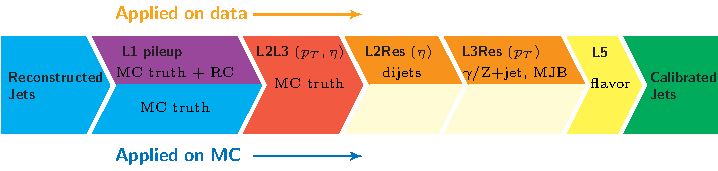
\includegraphics[width=\textwidth]{images/CMS_JEC_levels.pdf}
			}
			\label{fig:factorized_approach}
		\end{figure}
	\end{textblock}
	\vspace*{2.4cm}
	\begin{block}{MC-truth $\eta$ \& $p_{T}$ Corrections}
		\begin{itemize}
			\footnotesize
			\item L2Relative \& L3Absolute corrections seek to make the jet response flat vs $p_{T}$ and $\eta$
			\item During this step jets are corrected back to particle level so that the corrected jet $p_{T}$ is equal, on average, to the GenJet $p_{T}$
			\item Every effort is taken to make these corrections independent of the jet $p_{T}$ spectrum
			\item Derived on a QCD sample, but must be applicable to all physics processes
		\end{itemize}			
	\end{block}
	\vspace*{-0.15cm}
	\begin{alertblock}{Bombshell \#1}
		\footnotesize
		\begin{itemize}
			\item The L2Relative \& L3Absolute corrections are derived in one step
			\item They used to be separate, but we have combined them into one set of constants contained in the L2Relative payload
			\item The L3Absolute payload now contains a multiplicative factor of one, but is still there for future use
		\end{itemize}
	\end{alertblock}
	
	\begin{textblock}{.9}(0.05,.25)
		\begin{figure}
			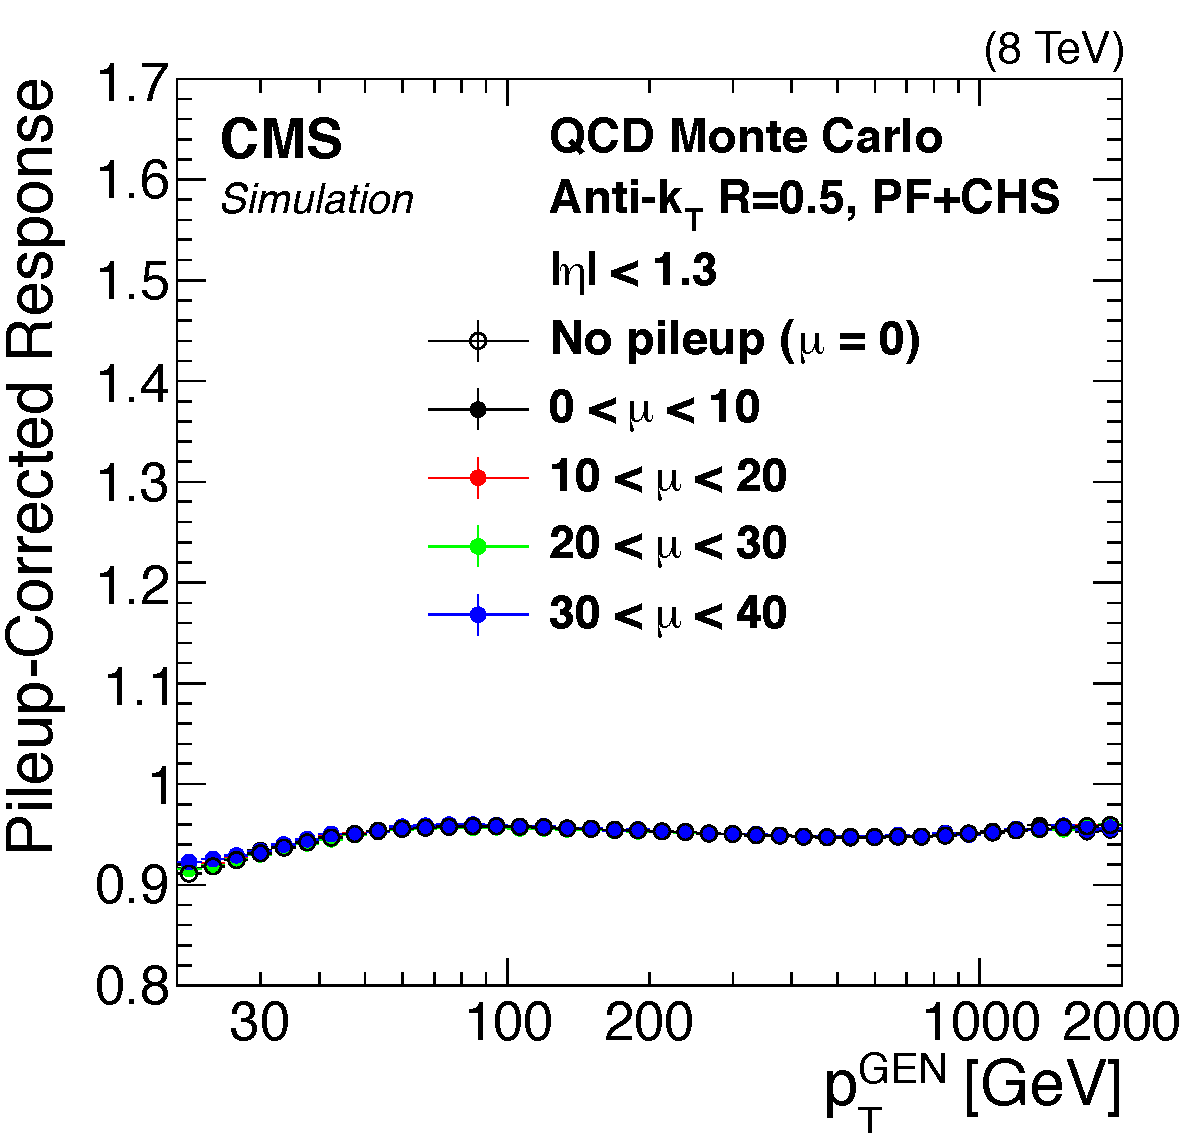
\includegraphics[width=0.5\textwidth]{images/Can1_noPreliminary.pdf} %no 13 TeV version
			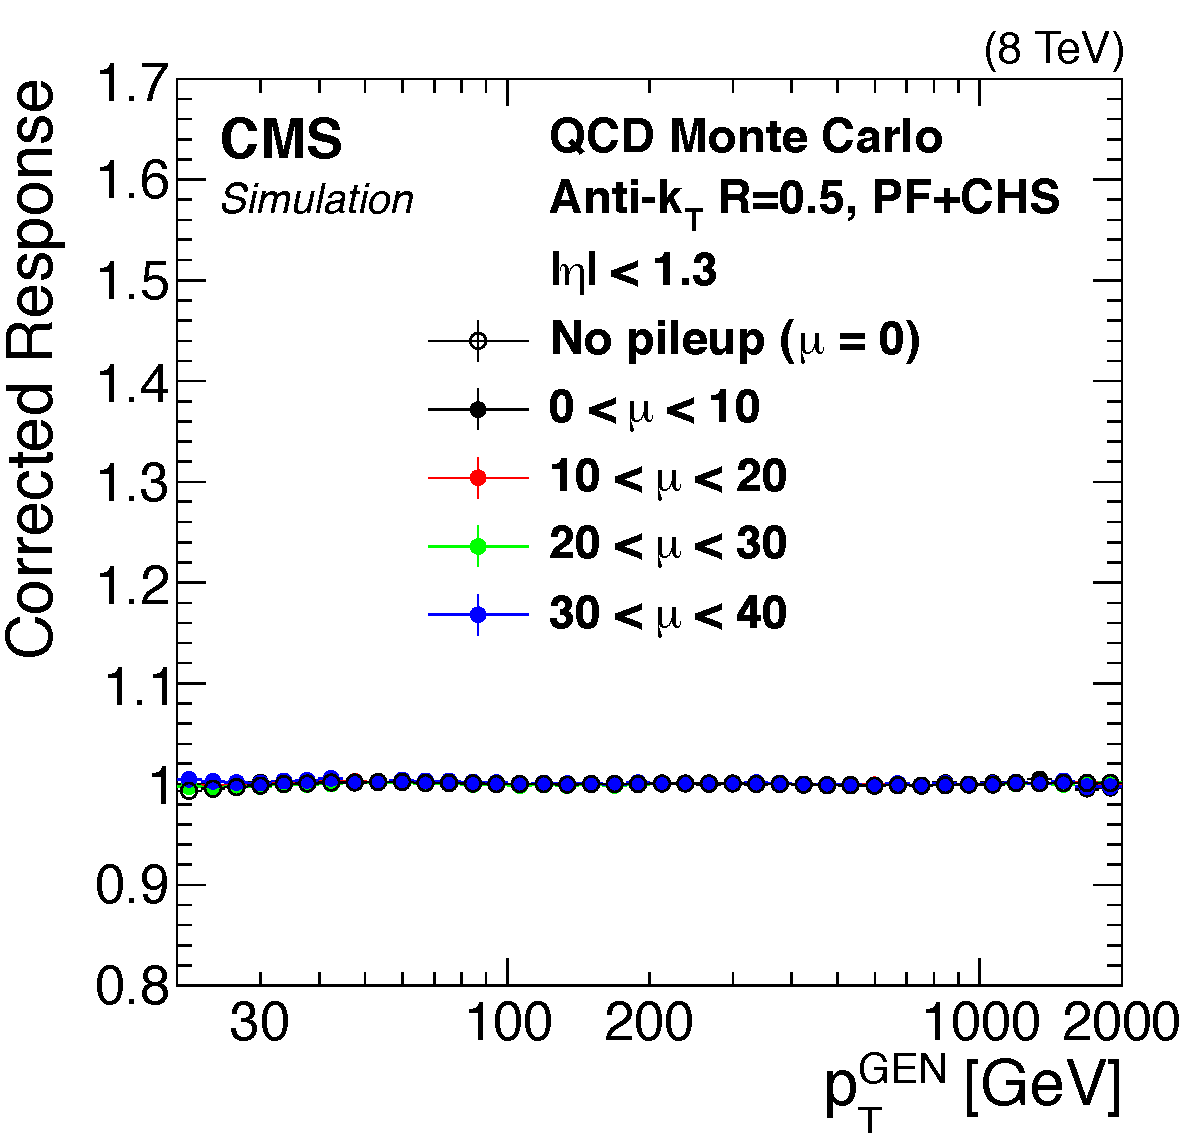
\includegraphics[width=0.5\textwidth]{images/Can2_noPreliminary.pdf} %no 13 TeV version
			\label{fig:closurel1l2l3}
		\end{figure}
	\end{textblock}
		\begin{textblock}{.9}(0.05,.25)
		\begin{figure}
			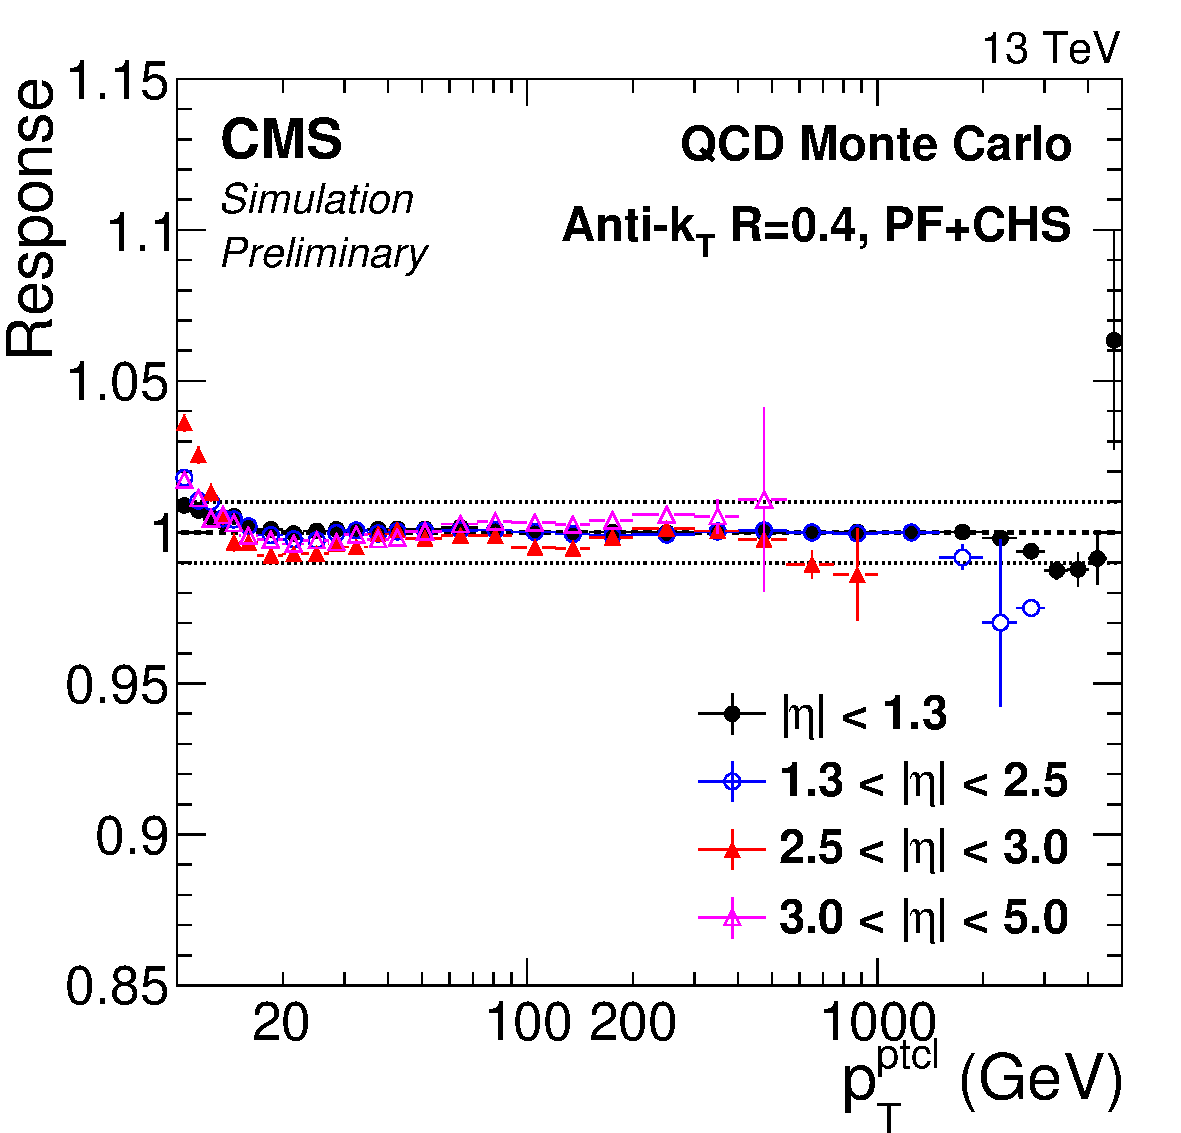
\includegraphics[width=0.5\textwidth]{images/JME-16-001/ClosureVsRefPt_Overview_ak4pfchs_no2000_afterL1L2L3.pdf}
		\end{figure}
	\end{textblock}
}
%---------------------------------------------------------------------------------------------------------------------------------------
\frame{
	\frametitle{JECs: A Factorized Approach}
        \begin{textblock}{.9}(0.05,0.085)
		\begin{figure}
			\scalebox{.9}{
			%	\documentclass[dvipsnames]{standalone}
\usepackage{color}
\usepackage{tikz}
\usetikzlibrary{arrows,shapes,shapes.multipart,backgrounds,calc,decorations.text,decorations.pathreplacing,matrix,shadings}
\tikzstyle{every picture}+=[remember picture]
\tikzstyle{na} = [baseline=-.5ex]

\begin{document}

\tikzstyle{levels} = [rectangle, draw, text width=6em, text centered, rounded corners, minimum height=2em, midway, shading=radial,outer color=Gray,middle color=white,inner color=white, Gray]
\tikzstyle{arrow} = [draw, -latex']
\tikzstyle{line} = [draw, -]

\newcommand*{\mytextstyle}{\sffamily\Large\bfseries\color{black!85}}
\newcommand{\myarrowstart}[9]{%
% inner radius, middle radius, outer radius, start angle,
% end angle, tip protusion angle, options, text
  \pgfmathsetmacro{\start}{#1}
  \pgfmathsetmacro{\rin}{#2}
  \pgfmathsetmacro{\rmid}{#3}
  \pgfmathsetmacro{\rout}{#4}
  \pgfmathsetmacro{\astart}{#5}
  \pgfmathsetmacro{\aend}{#6}
  \pgfmathsetmacro{\atip}{#7}
  \fill[#8] (\start+\astart,\rin) -- (\start+\aend,\rin) -- (\start+\aend+\atip,\rmid)
        -- (\start+\aend,\rout) -- (\start+\astart,\rout) -- (\start+\astart,\rmid)
        -- cycle;
  \node[font = \sffamily, align=center,text width=\aend-\astart,anchor = west, yshift=-0.0ex] (arrowend) at (\start+\astart,\rmid) {\mytextstyle{#9}};
%  \path[font = \sffamily, decoration = {text along path, text = {|\mytextstyle|#9},
%    text align = {align = center}, raise = -0.5ex}, decorate]
%    (\start+\astart+0.4*\atip,\rmid) -- (\start+\aend+0.4*\atip,\rmid);
}
\newcommand{\myarrow}[9]{%
% inner radius, middle radius, outer radius, start angle,
% end angle, tip protusion angle, options, text
  \pgfmathsetmacro{\start}{#1}
  \pgfmathsetmacro{\rin}{#2}
  \pgfmathsetmacro{\rmid}{#3}
  \pgfmathsetmacro{\rout}{#4}
  \pgfmathsetmacro{\astart}{#5}
  \pgfmathsetmacro{\aend}{#6}
  \pgfmathsetmacro{\atip}{#7}
  \fill[#8] (\start+\astart,\rin) -- (\start+\aend,\rin) -- (\start+\aend+\atip,\rmid) 
        -- (\start+\aend,\rout) -- (\start+\astart,\rout) -- (\start+\astart+\atip,\rmid)
        -- cycle;
  \path[font = \sffamily, decoration = {text along path, text = {|\mytextstyle|#9},
    text align = {align = center}, raise = -0.5ex}, decorate]
    (\start+\astart+0.75*\atip,\rmid) -- (\start+\aend+0.75*\atip,\rmid);
}
\newcommand{\myuphalfarrow}[9]{%
% inner radius, middle radius, outer radius, start angle,
% end angle, tip protusion angle, options, text
  \pgfmathsetmacro{\start}{#1}
  \pgfmathsetmacro{\rin}{#2}
  \pgfmathsetmacro{\rmid}{#3}
  \pgfmathsetmacro{\rout}{#4}
  \pgfmathsetmacro{\astart}{#5}
  \pgfmathsetmacro{\aend}{#6}
  \pgfmathsetmacro{\atip}{#7}
  \fill[#8] (\start+\astart,\rout) -- (\start+\aend,\rout) -- (\start+\aend+\atip,\rin) 
        -- (\start+\astart+\atip,\rin) -- cycle;
  \path[font = \sffamily, decoration = {text along path, text = {|\mytextstyle|#9},
    text align = {align = center}, raise = -0.5ex}, decorate]
    (\start+\astart+0.4*\atip,\rmid) -- (\start+\aend+0.4*\atip,\rmid);
}
\newcommand{\mylowhalfarrow}[9]{%
% inner radius, middle radius, outer radius, start angle,
% end angle, tip protusion angle, options, text
  \pgfmathsetmacro{\start}{#1}
  \pgfmathsetmacro{\rin}{#2}
  \pgfmathsetmacro{\rmid}{#3}
  \pgfmathsetmacro{\rout}{#4}
  \pgfmathsetmacro{\astart}{#5}
  \pgfmathsetmacro{\aend}{#6}
  \pgfmathsetmacro{\atip}{#7}
  \fill[#8] (\start+\astart+\atip,\rin) -- (\start+\aend+\atip,\rin) -- (\start+\aend,\rout)
        -- (\start+\astart,\rout) -- cycle;
  \path[font = \sffamily, decoration = {text along path, text = {|\mytextstyle|#9},
    text align = {align = center}, raise = -0.5ex}, decorate]
    (\start+\astart+0.4*\atip,\rmid) -- (\start+\aend+0.4*\atip,\rmid);
}
\newcommand{\myarrowend}[9]{%
% inner radius, middle radius, outer radius, start angle,
% end angle, tip protusion angle, options, text
  \pgfmathsetmacro{\start}{#1}
  \pgfmathsetmacro{\rin}{#2}
  \pgfmathsetmacro{\rmid}{#3}
  \pgfmathsetmacro{\rout}{#4}
  \pgfmathsetmacro{\astart}{#5}
  \pgfmathsetmacro{\aend}{#6}
  \pgfmathsetmacro{\atip}{#7}
  \fill[#8] (\start+\astart,\rin) -- (\start+\aend,\rin) -- (\start+\aend,\rmid)
        -- (\start+\aend,\rout) -- (\start+\astart,\rout) -- (\start+\astart+\atip,\rmid)
        -- cycle;
  \node[font = \sffamily, align=center,text width=\aend-\astart,anchor = west, yshift=-0.0ex] (arrowend) at (\start+\astart+0.75*\atip,\rmid) {\mytextstyle{#9}};
}

\begin{tikzpicture}[node distance = 2cm, auto, scale=0.8]
\scriptsize
    % Place nodes
    \myarrowstart{0}{0.5}{1.5}{2.5}{0}{1.75}{0.5}{Cyan,draw = Cyan, very thick}{\scriptsize{Reconstructed Jets}}

    \myuphalfarrow{1.95}{1.52}{1.75}{2.5}{0}{2.0}{0.5}{Purple,draw = Purple, very thick}{|\scriptsize|{MC + RC}}
    \mylowhalfarrow{1.95}{1.48}{1.}{0.5}{0}{2.0}{0.5}{Cyan,draw = Cyan, very thick}{|\scriptsize|{MC}}

    \node [font = \sffamily, align=left,text width=2.cm,anchor = west, yshift=-0.0ex] (l1data) at (2.4,2.2) {\mytextstyle\small\color{Black}\scriptsize{Pileup}};


    \myarrow{4.15}{0.5}{1.5}{2.5}{0}{2.95}{0.5}{Red!80,draw = Red!80, very thick}{|\scriptsize|{MC}}
    \node [font = \sffamily, align=left,text width=2.cm,anchor = west, yshift=-0.0ex] (l2l3) at (4.35,2.2) {\mytextstyle\small\color{Black}\scriptsize{Response $(p_{T},\eta)$ }};


    \myuphalfarrow{7.3}{1.52}{1.75}{2.5}{0}{1.9}{0.5}{BurntOrange,draw = BurntOrange, very thick}{|\scriptsize|{dijets}}
    \node [font = \sffamily, align=left,text width=2.cm,anchor = west, yshift=-0.0ex] (l2res) at (7.4,2.2) {\mytextstyle\small\color{Black}\scriptsize{Residuals$(\eta)$}};
    \mylowhalfarrow{7.3}{1.48}{1.25}{0.5}{0}{1.9}{0.5}{yellow!20,draw = yellow!20, very thick}{}


   \myuphalfarrow{9.4}{1.52}{1.75}{2.5}{0}{2.4}{0.5}{BurntOrange,draw = BurntOrange, very thick}{|\scriptsize|{   $\gamma$/Z$+$jet, MJB}}
    \node [font = \sffamily, align=left,text width=2.cm,anchor = west, yshift=-0.0ex] (l3res) at (9.6,2.2) {\mytextstyle\small\color{Black}\scriptsize{Residuals$(p_T)$}};
    \mylowhalfarrow{9.4}{1.48}{1.25}{0.5}{0}{2.4}{0.5}{yellow!20,draw = yellow!20, very thick}{}

 
   \myarrow{12.0}{0.5}{1.5}{2.5}{0}{1.}{0.5}{Yellow!80,draw = Yellow!80, very thick}{|\scriptsize|{MC}}
    \node [font = \sffamily, align=left,text width=2.cm,anchor = west, yshift=-0.0ex] (l5) at (12.,2.2) {\mytextstyle\small\color{Black}\scriptsize{ Flavor}};


    \myarrowend{13.20}{0.5}{1.5}{2.5}{0}{2.}{0.5}{Green!90,draw = Green!90, very thick}{\scriptsize{Calibrated Jets}}
    
    \node [font = \sffamily, align=left,text width=2.75cm,anchor = west, yshift=-0.0ex] (MC) at (2.25,0.) {\mytextstyle\small\color{RoyalBlue}Applied on MC};
    \node [font = \sffamily, align=left,text width=2.75cm,anchor = west, yshift=-0.0ex] (DATA) at (2.25,3.) {\mytextstyle\small\color{YellowOrange}Applied on data};

    \node [font = \sffamily, align=left,text width=5cm,anchor = west, yshift=-0.0ex] (INSITU) at (7.6,3.) %%{\mytextstyle\footnotesize{From in-situ MPF/Z-jet, flat in $p_{T}$}};
   {\mytextstyle\footnotesize{}};
    \node [font = \sffamily, align=left,text width=5cm,anchor = west, yshift=-0.0ex] (STARTBRACE) at (7.6,0.) {};
    \node [font = \sffamily, align=left,text width=5cm,anchor = west, yshift=-0.0ex] (ENDBRACE) at (12.65,0.5) {};
    \path[arrow,YellowOrange,thick, shorten <= -0.5cm] (DATA) -- (INSITU);
%    \draw [thick, decorate, decoration = {brace, amplitude = 10pt, mirror}, xshift = 0pt, yshift = 0pt] (7.25,0.75) -- (12.0,0.75) node [black, midway, xshift = 0cm, yshift = -0.8cm] {\mytextstyle\small{stuff}};
 %   \draw [thick, decorate, decoration = {brace, amplitude = 10pt, mirror}, xshift = 0pt, yshift = 0pt] (7.7,0.75) -- (12.65,0.75) node [levels, xshift = 0cm, yshift = -1.0cm] {\mytextstyle\scriptsize{L2L3Res}};

   \path[arrow,RoyalBlue,thick, shorten <= -0.5cm] (MC) -- (STARTBRACE);

 %   \node [levels, below of=MC, xshift = 3.6cm, yshift = 1.85cm, thick] (L1) {\mytextstyle\small{L1}};
 %   \node [levels, right of=L1, xshift = 4.4cm, yshift = -0.15cm, thick] (L2L3) {\mytextstyle\small{L2L3}};
\end{tikzpicture}

\end{document}

				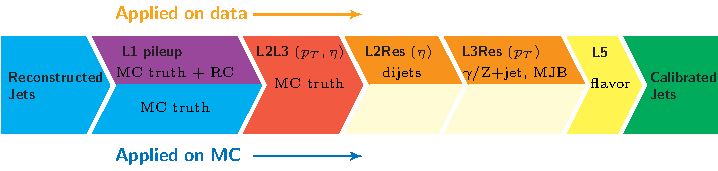
\includegraphics[width=\textwidth]{images/CMS_JEC_levels.pdf}
			}
			\label{fig:factorized_approach}
		\end{figure}
	\end{textblock}
	\vspace*{2.4cm}
%	\begin{block}{Electromagnetic Energy Fraction Correction}
%		\begin{itemize}
%			\footnotesize
%			\item The goal of the \textbf{defunct} L4 correction was to make the jet reponse uniform vs electromagnetic fraction
%		\end{itemize}
%	\end{block}
%	\vspace*{-0.15cm}
	\begin{block}{Jet Flavor Correction}
		\begin{itemize}
		\footnotesize
		\item The goal of this step is to correct for the jet flavor dependence
		\item The L1+L2+L3 corrections scale the energy of an ``average QCD jet" back to the energy of the corresponding generator level particle jet
		\begin{itemize}
			\footnotesize
			\item Application of the generic L1+L2+L3 corrections to jets with a flavor composition different than that of QCD jets leads to an over- or under-corection
		\end{itemize}
		\item L5Flavor corrections are applied on top of the default L1+L2+L3 jet correction and corrects the jet energy back to particle level
			\begin{itemize}
				\footnotesize
				\item L5 corrections act at the particle level. If corrections back to the parton level are required, the L1+L2+L3+L5 corrections can be combined with the L7 corrections
				\item L5 corrections provide corrections only relative to the ``typical" mix of flavors present in the sample that they have been derived from
				\item Currently derived on QCD events, but can also be made from top-quark pair events
			\end{itemize}
		\end{itemize}
	\end{block}
}
%---------------------------------------------------------------------------------------------------------------------------------------
\frame{
	\frametitle{JECs: A Factorized Approach}
        \begin{textblock}{.9}(0.05,0.085)
		\begin{figure}
			\scalebox{.9}{
			%	\documentclass[dvipsnames]{standalone}
\usepackage{color}
\usepackage{tikz}
\usetikzlibrary{arrows,shapes,shapes.multipart,backgrounds,calc,decorations.text,decorations.pathreplacing,matrix,shadings}
\tikzstyle{every picture}+=[remember picture]
\tikzstyle{na} = [baseline=-.5ex]

\begin{document}

\tikzstyle{levels} = [rectangle, draw, text width=6em, text centered, rounded corners, minimum height=2em, midway, shading=radial,outer color=Gray,middle color=white,inner color=white, Gray]
\tikzstyle{arrow} = [draw, -latex']
\tikzstyle{line} = [draw, -]

\newcommand*{\mytextstyle}{\sffamily\Large\bfseries\color{black!85}}
\newcommand{\myarrowstart}[9]{%
% inner radius, middle radius, outer radius, start angle,
% end angle, tip protusion angle, options, text
  \pgfmathsetmacro{\start}{#1}
  \pgfmathsetmacro{\rin}{#2}
  \pgfmathsetmacro{\rmid}{#3}
  \pgfmathsetmacro{\rout}{#4}
  \pgfmathsetmacro{\astart}{#5}
  \pgfmathsetmacro{\aend}{#6}
  \pgfmathsetmacro{\atip}{#7}
  \fill[#8] (\start+\astart,\rin) -- (\start+\aend,\rin) -- (\start+\aend+\atip,\rmid)
        -- (\start+\aend,\rout) -- (\start+\astart,\rout) -- (\start+\astart,\rmid)
        -- cycle;
  \node[font = \sffamily, align=center,text width=\aend-\astart,anchor = west, yshift=-0.0ex] (arrowend) at (\start+\astart,\rmid) {\mytextstyle{#9}};
%  \path[font = \sffamily, decoration = {text along path, text = {|\mytextstyle|#9},
%    text align = {align = center}, raise = -0.5ex}, decorate]
%    (\start+\astart+0.4*\atip,\rmid) -- (\start+\aend+0.4*\atip,\rmid);
}
\newcommand{\myarrow}[9]{%
% inner radius, middle radius, outer radius, start angle,
% end angle, tip protusion angle, options, text
  \pgfmathsetmacro{\start}{#1}
  \pgfmathsetmacro{\rin}{#2}
  \pgfmathsetmacro{\rmid}{#3}
  \pgfmathsetmacro{\rout}{#4}
  \pgfmathsetmacro{\astart}{#5}
  \pgfmathsetmacro{\aend}{#6}
  \pgfmathsetmacro{\atip}{#7}
  \fill[#8] (\start+\astart,\rin) -- (\start+\aend,\rin) -- (\start+\aend+\atip,\rmid) 
        -- (\start+\aend,\rout) -- (\start+\astart,\rout) -- (\start+\astart+\atip,\rmid)
        -- cycle;
  \path[font = \sffamily, decoration = {text along path, text = {|\mytextstyle|#9},
    text align = {align = center}, raise = -0.5ex}, decorate]
    (\start+\astart+0.75*\atip,\rmid) -- (\start+\aend+0.75*\atip,\rmid);
}
\newcommand{\myuphalfarrow}[9]{%
% inner radius, middle radius, outer radius, start angle,
% end angle, tip protusion angle, options, text
  \pgfmathsetmacro{\start}{#1}
  \pgfmathsetmacro{\rin}{#2}
  \pgfmathsetmacro{\rmid}{#3}
  \pgfmathsetmacro{\rout}{#4}
  \pgfmathsetmacro{\astart}{#5}
  \pgfmathsetmacro{\aend}{#6}
  \pgfmathsetmacro{\atip}{#7}
  \fill[#8] (\start+\astart,\rout) -- (\start+\aend,\rout) -- (\start+\aend+\atip,\rin) 
        -- (\start+\astart+\atip,\rin) -- cycle;
  \path[font = \sffamily, decoration = {text along path, text = {|\mytextstyle|#9},
    text align = {align = center}, raise = -0.5ex}, decorate]
    (\start+\astart+0.4*\atip,\rmid) -- (\start+\aend+0.4*\atip,\rmid);
}
\newcommand{\mylowhalfarrow}[9]{%
% inner radius, middle radius, outer radius, start angle,
% end angle, tip protusion angle, options, text
  \pgfmathsetmacro{\start}{#1}
  \pgfmathsetmacro{\rin}{#2}
  \pgfmathsetmacro{\rmid}{#3}
  \pgfmathsetmacro{\rout}{#4}
  \pgfmathsetmacro{\astart}{#5}
  \pgfmathsetmacro{\aend}{#6}
  \pgfmathsetmacro{\atip}{#7}
  \fill[#8] (\start+\astart+\atip,\rin) -- (\start+\aend+\atip,\rin) -- (\start+\aend,\rout)
        -- (\start+\astart,\rout) -- cycle;
  \path[font = \sffamily, decoration = {text along path, text = {|\mytextstyle|#9},
    text align = {align = center}, raise = -0.5ex}, decorate]
    (\start+\astart+0.4*\atip,\rmid) -- (\start+\aend+0.4*\atip,\rmid);
}
\newcommand{\myarrowend}[9]{%
% inner radius, middle radius, outer radius, start angle,
% end angle, tip protusion angle, options, text
  \pgfmathsetmacro{\start}{#1}
  \pgfmathsetmacro{\rin}{#2}
  \pgfmathsetmacro{\rmid}{#3}
  \pgfmathsetmacro{\rout}{#4}
  \pgfmathsetmacro{\astart}{#5}
  \pgfmathsetmacro{\aend}{#6}
  \pgfmathsetmacro{\atip}{#7}
  \fill[#8] (\start+\astart,\rin) -- (\start+\aend,\rin) -- (\start+\aend,\rmid)
        -- (\start+\aend,\rout) -- (\start+\astart,\rout) -- (\start+\astart+\atip,\rmid)
        -- cycle;
  \node[font = \sffamily, align=center,text width=\aend-\astart,anchor = west, yshift=-0.0ex] (arrowend) at (\start+\astart+0.75*\atip,\rmid) {\mytextstyle{#9}};
}

\begin{tikzpicture}[node distance = 2cm, auto, scale=0.8]
\scriptsize
    % Place nodes
    \myarrowstart{0}{0.5}{1.5}{2.5}{0}{1.75}{0.5}{Cyan,draw = Cyan, very thick}{\scriptsize{Reconstructed Jets}}

    \myuphalfarrow{1.95}{1.52}{1.75}{2.5}{0}{2.0}{0.5}{Purple,draw = Purple, very thick}{|\scriptsize|{MC + RC}}
    \mylowhalfarrow{1.95}{1.48}{1.}{0.5}{0}{2.0}{0.5}{Cyan,draw = Cyan, very thick}{|\scriptsize|{MC}}

    \node [font = \sffamily, align=left,text width=2.cm,anchor = west, yshift=-0.0ex] (l1data) at (2.4,2.2) {\mytextstyle\small\color{Black}\scriptsize{Pileup}};


    \myarrow{4.15}{0.5}{1.5}{2.5}{0}{2.95}{0.5}{Red!80,draw = Red!80, very thick}{|\scriptsize|{MC}}
    \node [font = \sffamily, align=left,text width=2.cm,anchor = west, yshift=-0.0ex] (l2l3) at (4.35,2.2) {\mytextstyle\small\color{Black}\scriptsize{Response $(p_{T},\eta)$ }};


    \myuphalfarrow{7.3}{1.52}{1.75}{2.5}{0}{1.9}{0.5}{BurntOrange,draw = BurntOrange, very thick}{|\scriptsize|{dijets}}
    \node [font = \sffamily, align=left,text width=2.cm,anchor = west, yshift=-0.0ex] (l2res) at (7.4,2.2) {\mytextstyle\small\color{Black}\scriptsize{Residuals$(\eta)$}};
    \mylowhalfarrow{7.3}{1.48}{1.25}{0.5}{0}{1.9}{0.5}{yellow!20,draw = yellow!20, very thick}{}


   \myuphalfarrow{9.4}{1.52}{1.75}{2.5}{0}{2.4}{0.5}{BurntOrange,draw = BurntOrange, very thick}{|\scriptsize|{   $\gamma$/Z$+$jet, MJB}}
    \node [font = \sffamily, align=left,text width=2.cm,anchor = west, yshift=-0.0ex] (l3res) at (9.6,2.2) {\mytextstyle\small\color{Black}\scriptsize{Residuals$(p_T)$}};
    \mylowhalfarrow{9.4}{1.48}{1.25}{0.5}{0}{2.4}{0.5}{yellow!20,draw = yellow!20, very thick}{}

 
   \myarrow{12.0}{0.5}{1.5}{2.5}{0}{1.}{0.5}{Yellow!80,draw = Yellow!80, very thick}{|\scriptsize|{MC}}
    \node [font = \sffamily, align=left,text width=2.cm,anchor = west, yshift=-0.0ex] (l5) at (12.,2.2) {\mytextstyle\small\color{Black}\scriptsize{ Flavor}};


    \myarrowend{13.20}{0.5}{1.5}{2.5}{0}{2.}{0.5}{Green!90,draw = Green!90, very thick}{\scriptsize{Calibrated Jets}}
    
    \node [font = \sffamily, align=left,text width=2.75cm,anchor = west, yshift=-0.0ex] (MC) at (2.25,0.) {\mytextstyle\small\color{RoyalBlue}Applied on MC};
    \node [font = \sffamily, align=left,text width=2.75cm,anchor = west, yshift=-0.0ex] (DATA) at (2.25,3.) {\mytextstyle\small\color{YellowOrange}Applied on data};

    \node [font = \sffamily, align=left,text width=5cm,anchor = west, yshift=-0.0ex] (INSITU) at (7.6,3.) %%{\mytextstyle\footnotesize{From in-situ MPF/Z-jet, flat in $p_{T}$}};
   {\mytextstyle\footnotesize{}};
    \node [font = \sffamily, align=left,text width=5cm,anchor = west, yshift=-0.0ex] (STARTBRACE) at (7.6,0.) {};
    \node [font = \sffamily, align=left,text width=5cm,anchor = west, yshift=-0.0ex] (ENDBRACE) at (12.65,0.5) {};
    \path[arrow,YellowOrange,thick, shorten <= -0.5cm] (DATA) -- (INSITU);
%    \draw [thick, decorate, decoration = {brace, amplitude = 10pt, mirror}, xshift = 0pt, yshift = 0pt] (7.25,0.75) -- (12.0,0.75) node [black, midway, xshift = 0cm, yshift = -0.8cm] {\mytextstyle\small{stuff}};
 %   \draw [thick, decorate, decoration = {brace, amplitude = 10pt, mirror}, xshift = 0pt, yshift = 0pt] (7.7,0.75) -- (12.65,0.75) node [levels, xshift = 0cm, yshift = -1.0cm] {\mytextstyle\scriptsize{L2L3Res}};

   \path[arrow,RoyalBlue,thick, shorten <= -0.5cm] (MC) -- (STARTBRACE);

 %   \node [levels, below of=MC, xshift = 3.6cm, yshift = 1.85cm, thick] (L1) {\mytextstyle\small{L1}};
 %   \node [levels, right of=L1, xshift = 4.4cm, yshift = -0.15cm, thick] (L2L3) {\mytextstyle\small{L2L3}};
\end{tikzpicture}

\end{document}

				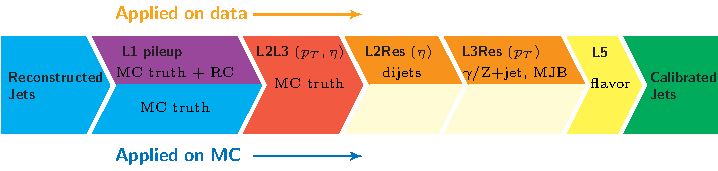
\includegraphics[width=\textwidth]{images/CMS_JEC_levels.pdf}
			}
			\label{fig:factorized_approach}
		\end{figure}
	\end{textblock}
	\vspace*{2.4cm}
%	\begin{block}{Electromagnetic Energy Fraction Correction}
%		\begin{itemize}
%			\footnotesize
%			\item The goal of the \textbf{defunct} L4 correction was to make the jet reponse uniform vs electromagnetic fraction
%		\end{itemize}
%	\end{block}
%	\vspace*{-0.15cm}
	\begin{block}{Jet Flavor Correction}
		\begin{itemize}
		\footnotesize
		\item The goal of this step is to correct for the jet flavor dependence
		\item The L1+L2+L3 corrections scale the energy of an ``average QCD jet" back to the energy of the corresponding generator level particle jet
		\begin{itemize}
			\footnotesize
			\item Application of the generic L1+L2+L3 corrections to jets with a flavor composition different than that of QCD jets leads to an over- or under-corection
		\end{itemize}
		\item L5Flavor corrections are applied on top of the default L1+L2+L3 jet correction and corrects the jet energy back to particle level
			\begin{itemize}
				\footnotesize
				\item L5 corrections act at the particle level. If corrections back to the parton level are required, the L1+L2+L3+L5 corrections can be combined with the L7 corrections
				\item L5 corrections provide corrections only relative to the ``typical" mix of flavors present in the sample that they have been derived from
				\item Currently derived on QCD events, but can also be made from top-quark pair events
			\end{itemize}
		\end{itemize}
	\end{block}
	
		\begin{textblock}{.9}(0.05,.25)
		\begin{figure}
			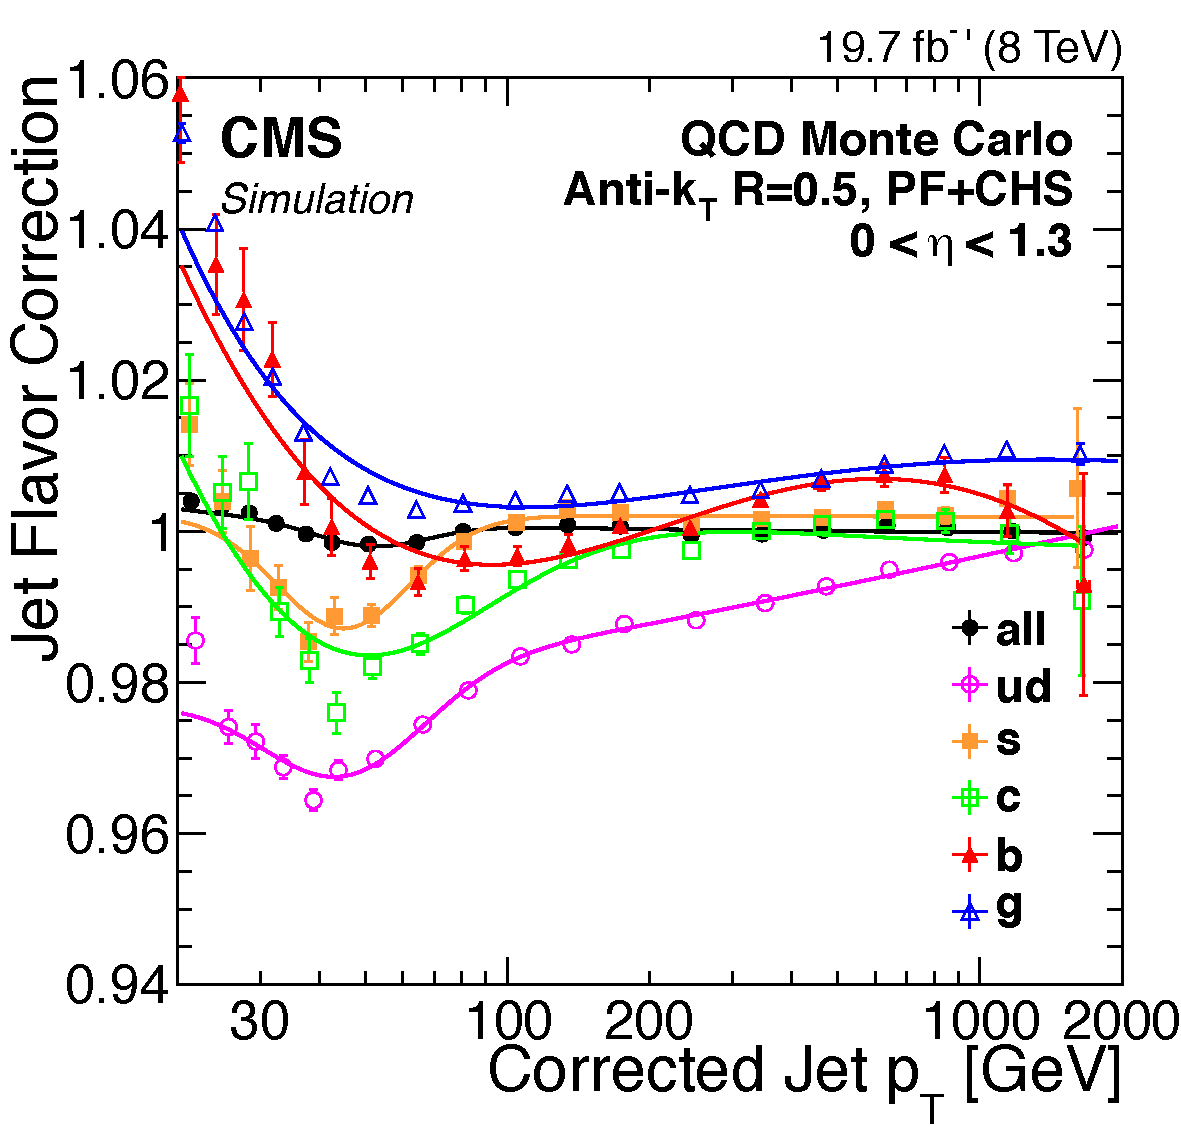
\includegraphics[width=0.5\textwidth]{images/L5AbsCorGraphs.pdf}  %no 13 TeV version
			\label{fig:flavor}
		\end{figure}
	\end{textblock}
}
%---------------------------------------------------------------------------------------------------------------------------------------
\frame{
	\frametitle{JECs: A Factorized Approach}
        \begin{textblock}{.9}(0.05,0.085)
		\begin{figure}
			\scalebox{.9}{
			%	\documentclass[dvipsnames]{standalone}
\usepackage{color}
\usepackage{tikz}
\usetikzlibrary{arrows,shapes,shapes.multipart,backgrounds,calc,decorations.text,decorations.pathreplacing,matrix,shadings}
\tikzstyle{every picture}+=[remember picture]
\tikzstyle{na} = [baseline=-.5ex]

\begin{document}

\tikzstyle{levels} = [rectangle, draw, text width=6em, text centered, rounded corners, minimum height=2em, midway, shading=radial,outer color=Gray,middle color=white,inner color=white, Gray]
\tikzstyle{arrow} = [draw, -latex']
\tikzstyle{line} = [draw, -]

\newcommand*{\mytextstyle}{\sffamily\Large\bfseries\color{black!85}}
\newcommand{\myarrowstart}[9]{%
% inner radius, middle radius, outer radius, start angle,
% end angle, tip protusion angle, options, text
  \pgfmathsetmacro{\start}{#1}
  \pgfmathsetmacro{\rin}{#2}
  \pgfmathsetmacro{\rmid}{#3}
  \pgfmathsetmacro{\rout}{#4}
  \pgfmathsetmacro{\astart}{#5}
  \pgfmathsetmacro{\aend}{#6}
  \pgfmathsetmacro{\atip}{#7}
  \fill[#8] (\start+\astart,\rin) -- (\start+\aend,\rin) -- (\start+\aend+\atip,\rmid)
        -- (\start+\aend,\rout) -- (\start+\astart,\rout) -- (\start+\astart,\rmid)
        -- cycle;
  \node[font = \sffamily, align=center,text width=\aend-\astart,anchor = west, yshift=-0.0ex] (arrowend) at (\start+\astart,\rmid) {\mytextstyle{#9}};
%  \path[font = \sffamily, decoration = {text along path, text = {|\mytextstyle|#9},
%    text align = {align = center}, raise = -0.5ex}, decorate]
%    (\start+\astart+0.4*\atip,\rmid) -- (\start+\aend+0.4*\atip,\rmid);
}
\newcommand{\myarrow}[9]{%
% inner radius, middle radius, outer radius, start angle,
% end angle, tip protusion angle, options, text
  \pgfmathsetmacro{\start}{#1}
  \pgfmathsetmacro{\rin}{#2}
  \pgfmathsetmacro{\rmid}{#3}
  \pgfmathsetmacro{\rout}{#4}
  \pgfmathsetmacro{\astart}{#5}
  \pgfmathsetmacro{\aend}{#6}
  \pgfmathsetmacro{\atip}{#7}
  \fill[#8] (\start+\astart,\rin) -- (\start+\aend,\rin) -- (\start+\aend+\atip,\rmid) 
        -- (\start+\aend,\rout) -- (\start+\astart,\rout) -- (\start+\astart+\atip,\rmid)
        -- cycle;
  \path[font = \sffamily, decoration = {text along path, text = {|\mytextstyle|#9},
    text align = {align = center}, raise = -0.5ex}, decorate]
    (\start+\astart+0.75*\atip,\rmid) -- (\start+\aend+0.75*\atip,\rmid);
}
\newcommand{\myuphalfarrow}[9]{%
% inner radius, middle radius, outer radius, start angle,
% end angle, tip protusion angle, options, text
  \pgfmathsetmacro{\start}{#1}
  \pgfmathsetmacro{\rin}{#2}
  \pgfmathsetmacro{\rmid}{#3}
  \pgfmathsetmacro{\rout}{#4}
  \pgfmathsetmacro{\astart}{#5}
  \pgfmathsetmacro{\aend}{#6}
  \pgfmathsetmacro{\atip}{#7}
  \fill[#8] (\start+\astart,\rout) -- (\start+\aend,\rout) -- (\start+\aend+\atip,\rin) 
        -- (\start+\astart+\atip,\rin) -- cycle;
  \path[font = \sffamily, decoration = {text along path, text = {|\mytextstyle|#9},
    text align = {align = center}, raise = -0.5ex}, decorate]
    (\start+\astart+0.4*\atip,\rmid) -- (\start+\aend+0.4*\atip,\rmid);
}
\newcommand{\mylowhalfarrow}[9]{%
% inner radius, middle radius, outer radius, start angle,
% end angle, tip protusion angle, options, text
  \pgfmathsetmacro{\start}{#1}
  \pgfmathsetmacro{\rin}{#2}
  \pgfmathsetmacro{\rmid}{#3}
  \pgfmathsetmacro{\rout}{#4}
  \pgfmathsetmacro{\astart}{#5}
  \pgfmathsetmacro{\aend}{#6}
  \pgfmathsetmacro{\atip}{#7}
  \fill[#8] (\start+\astart+\atip,\rin) -- (\start+\aend+\atip,\rin) -- (\start+\aend,\rout)
        -- (\start+\astart,\rout) -- cycle;
  \path[font = \sffamily, decoration = {text along path, text = {|\mytextstyle|#9},
    text align = {align = center}, raise = -0.5ex}, decorate]
    (\start+\astart+0.4*\atip,\rmid) -- (\start+\aend+0.4*\atip,\rmid);
}
\newcommand{\myarrowend}[9]{%
% inner radius, middle radius, outer radius, start angle,
% end angle, tip protusion angle, options, text
  \pgfmathsetmacro{\start}{#1}
  \pgfmathsetmacro{\rin}{#2}
  \pgfmathsetmacro{\rmid}{#3}
  \pgfmathsetmacro{\rout}{#4}
  \pgfmathsetmacro{\astart}{#5}
  \pgfmathsetmacro{\aend}{#6}
  \pgfmathsetmacro{\atip}{#7}
  \fill[#8] (\start+\astart,\rin) -- (\start+\aend,\rin) -- (\start+\aend,\rmid)
        -- (\start+\aend,\rout) -- (\start+\astart,\rout) -- (\start+\astart+\atip,\rmid)
        -- cycle;
  \node[font = \sffamily, align=center,text width=\aend-\astart,anchor = west, yshift=-0.0ex] (arrowend) at (\start+\astart+0.75*\atip,\rmid) {\mytextstyle{#9}};
}

\begin{tikzpicture}[node distance = 2cm, auto, scale=0.8]
\scriptsize
    % Place nodes
    \myarrowstart{0}{0.5}{1.5}{2.5}{0}{1.75}{0.5}{Cyan,draw = Cyan, very thick}{\scriptsize{Reconstructed Jets}}

    \myuphalfarrow{1.95}{1.52}{1.75}{2.5}{0}{2.0}{0.5}{Purple,draw = Purple, very thick}{|\scriptsize|{MC + RC}}
    \mylowhalfarrow{1.95}{1.48}{1.}{0.5}{0}{2.0}{0.5}{Cyan,draw = Cyan, very thick}{|\scriptsize|{MC}}

    \node [font = \sffamily, align=left,text width=2.cm,anchor = west, yshift=-0.0ex] (l1data) at (2.4,2.2) {\mytextstyle\small\color{Black}\scriptsize{Pileup}};


    \myarrow{4.15}{0.5}{1.5}{2.5}{0}{2.95}{0.5}{Red!80,draw = Red!80, very thick}{|\scriptsize|{MC}}
    \node [font = \sffamily, align=left,text width=2.cm,anchor = west, yshift=-0.0ex] (l2l3) at (4.35,2.2) {\mytextstyle\small\color{Black}\scriptsize{Response $(p_{T},\eta)$ }};


    \myuphalfarrow{7.3}{1.52}{1.75}{2.5}{0}{1.9}{0.5}{BurntOrange,draw = BurntOrange, very thick}{|\scriptsize|{dijets}}
    \node [font = \sffamily, align=left,text width=2.cm,anchor = west, yshift=-0.0ex] (l2res) at (7.4,2.2) {\mytextstyle\small\color{Black}\scriptsize{Residuals$(\eta)$}};
    \mylowhalfarrow{7.3}{1.48}{1.25}{0.5}{0}{1.9}{0.5}{yellow!20,draw = yellow!20, very thick}{}


   \myuphalfarrow{9.4}{1.52}{1.75}{2.5}{0}{2.4}{0.5}{BurntOrange,draw = BurntOrange, very thick}{|\scriptsize|{   $\gamma$/Z$+$jet, MJB}}
    \node [font = \sffamily, align=left,text width=2.cm,anchor = west, yshift=-0.0ex] (l3res) at (9.6,2.2) {\mytextstyle\small\color{Black}\scriptsize{Residuals$(p_T)$}};
    \mylowhalfarrow{9.4}{1.48}{1.25}{0.5}{0}{2.4}{0.5}{yellow!20,draw = yellow!20, very thick}{}

 
   \myarrow{12.0}{0.5}{1.5}{2.5}{0}{1.}{0.5}{Yellow!80,draw = Yellow!80, very thick}{|\scriptsize|{MC}}
    \node [font = \sffamily, align=left,text width=2.cm,anchor = west, yshift=-0.0ex] (l5) at (12.,2.2) {\mytextstyle\small\color{Black}\scriptsize{ Flavor}};


    \myarrowend{13.20}{0.5}{1.5}{2.5}{0}{2.}{0.5}{Green!90,draw = Green!90, very thick}{\scriptsize{Calibrated Jets}}
    
    \node [font = \sffamily, align=left,text width=2.75cm,anchor = west, yshift=-0.0ex] (MC) at (2.25,0.) {\mytextstyle\small\color{RoyalBlue}Applied on MC};
    \node [font = \sffamily, align=left,text width=2.75cm,anchor = west, yshift=-0.0ex] (DATA) at (2.25,3.) {\mytextstyle\small\color{YellowOrange}Applied on data};

    \node [font = \sffamily, align=left,text width=5cm,anchor = west, yshift=-0.0ex] (INSITU) at (7.6,3.) %%{\mytextstyle\footnotesize{From in-situ MPF/Z-jet, flat in $p_{T}$}};
   {\mytextstyle\footnotesize{}};
    \node [font = \sffamily, align=left,text width=5cm,anchor = west, yshift=-0.0ex] (STARTBRACE) at (7.6,0.) {};
    \node [font = \sffamily, align=left,text width=5cm,anchor = west, yshift=-0.0ex] (ENDBRACE) at (12.65,0.5) {};
    \path[arrow,YellowOrange,thick, shorten <= -0.5cm] (DATA) -- (INSITU);
%    \draw [thick, decorate, decoration = {brace, amplitude = 10pt, mirror}, xshift = 0pt, yshift = 0pt] (7.25,0.75) -- (12.0,0.75) node [black, midway, xshift = 0cm, yshift = -0.8cm] {\mytextstyle\small{stuff}};
 %   \draw [thick, decorate, decoration = {brace, amplitude = 10pt, mirror}, xshift = 0pt, yshift = 0pt] (7.7,0.75) -- (12.65,0.75) node [levels, xshift = 0cm, yshift = -1.0cm] {\mytextstyle\scriptsize{L2L3Res}};

   \path[arrow,RoyalBlue,thick, shorten <= -0.5cm] (MC) -- (STARTBRACE);

 %   \node [levels, below of=MC, xshift = 3.6cm, yshift = 1.85cm, thick] (L1) {\mytextstyle\small{L1}};
 %   \node [levels, right of=L1, xshift = 4.4cm, yshift = -0.15cm, thick] (L2L3) {\mytextstyle\small{L2L3}};
\end{tikzpicture}

\end{document}

				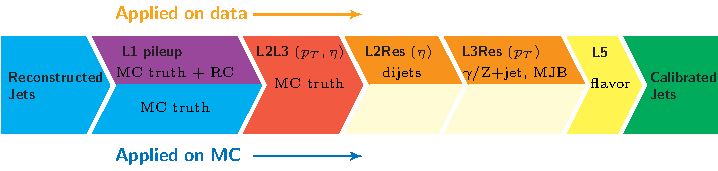
\includegraphics[width=\textwidth]{images/CMS_JEC_levels.pdf}
			}
			\label{fig:factorized_approach}
		\end{figure}
	\end{textblock}
	\vspace*{2.4cm}
	\begin{block}{Parton Jet Correction}
		\begin{itemize}
			\item The optional L7 parton correction is applied on top of the default L1+L2+L3 (L5) correction and corrects back to the parton level.
			\item This means that the corrected jet $p_{T}$ is equal to the originating parton $p_{T}$, on average More details \href{https://twiki.cern.ch/twiki/bin/view/CMS/IntroToJEC\#L7_Parton_Jet_Correction}{\color{blue}{here}}.
		\end{itemize}
	\end{block}

	\begin{block}{Residuals Corrections}
		\begin{itemize}
			\item The residual calibration of data:.
			\begin{itemize}
				\item First, the MC Truth L2L3 JEC calibration is applied, which takes care of the bulk of the energy response.
				\item Second, a small residual calibration ($\eta$ and $p_{T}$ dependent) is applied which fixes the small differences between data and MC.
			\end{itemize}
		\end{itemize}
	\end{block}
}
%---------------------------------------------------------------------------------------------------------------------------------------
\frame{
	\frametitle{Relative Corrections for Data}
	\framesubtitle{L2Residual Corrections ($\eta$)}
	\vspace*{-0.24cm}
	\begin{columns}[T]
		\column{0.4\textwidth}
			%\begin{textblock}{2.5}(0.25,2.0){\color{red}\scriptsize{(Dijet events)}}\end{textblock}
			\vspace*{-0.4cm}
			\begin{figure}[T]
				\centering
				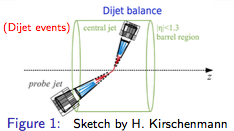
\includegraphics[width=0.9\textwidth]{images/RelativeCalibration.png}% 
				\vspace*{-0.4cm}
				%\caption{\footnotesize{Sketch by H. Kirschenmann}}
				\label{fig:RelativeCalibration}
			\end{figure}

			\begin{block}{}
				\begin{itemize}
					\footnotesize
                                      \item $\eta$-dependent correction  
                                      \item Two methods using dijet events: $p_T$ balance and MET Projection Fraction (MPF)
					\item Separate constants for outer end cap (very large data/MC difference) and HF (very small data/MC difference)
                                        \item \href{https://indico.cern.ch/event/544654/contributions/2210386/attachments/1296039/1937185/20160625_JEC_L2Res_CMSSW80X_2016Data_4_0fb_addJER.pdf}{\color{blue}\scriptsize{Latest results presented last week}}.  On right: MPF method with Pythia8
				\end{itemize}
			\end{block}
		\column{0.56\textwidth}
		\vspace*{-0.4cm}
		\begin{figure}[T]
			\centering
			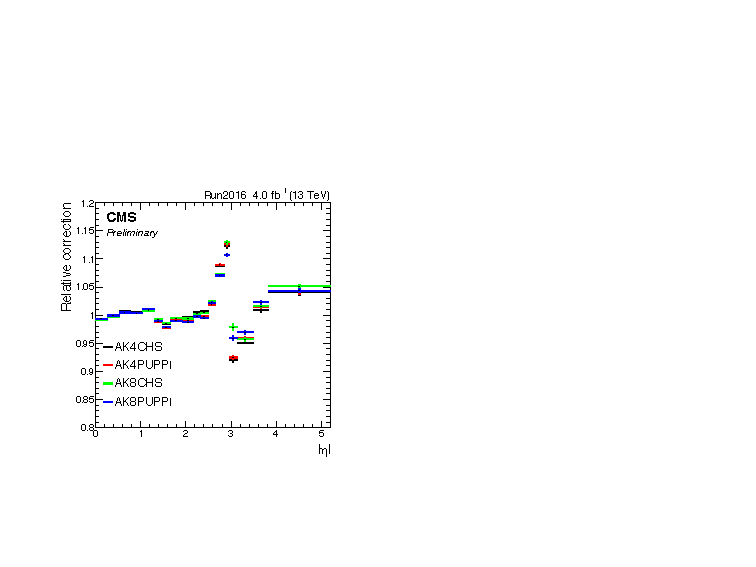
\includegraphics[width=6.5cm]{images/l2res.pdf}%  
			\label{fig:L2Residual}
		\end{figure}
	\end{columns}
}
%---------------------------------------------------------------------------------------------------------------------------------------
\frame{
	\frametitle{Corrections to Scale in Barrel Region}
	\framesubtitle{L3Residual Corrections ($p_T$)}
	\vspace*{-0.24cm}
	\begin{columns}[T]
		\column{0.5\textwidth}
			%\begin{textblock}{2.5}(0.25,1.5){\color{red}\scriptsize{$Z\left(\mu\mu\right)+jet$\\$Z\left(ee\right)+jet$\\$\gamma+jet$\\(multijet events)}}\end{textblock}
			\vspace*{-0.4cm}
			\begin{figure}[T]
				\centering
				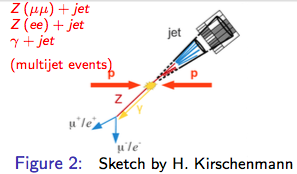
\includegraphics[width=1.0\textwidth]{images/unc2.png}%
				%\vspace*{-0.4cm}
%				\caption{\footnotesize{Sketch by H. Kirschenmann}}
				\label{fig:AbsoluteCalibration}
			\end{figure}

			\begin{block}{}
			\begin{itemize}
				\footnotesize
                                \item $p_T$-dependent correction
				\item Use $\gamma$+jet or $Z(\mu\mu/ee)$+jet events
                                \item Again use $p_T$ balancing or MPF methods
                                \item Latest \href{https://indico.cern.ch/event/544654/contributions/2210383/attachments/1295640/1936919/2016-06-22-JERC-virtual-meeting-cheidecker.pdf}{\color{blue}\scriptsize{Z+jet}} and \href{https://indico.cern.ch/event/544654/contributions/2210385/attachments/1296031/1932394/Giugno-21-2016_-_Federico_Preiato.pdf}{\color{blue}\scriptsize{$\gamma$+jet}} results presented last week.  On right: $Z(\mu\mu)+jet$
                                 \item Third method, Multijet Balance (MJB), using multijet events constrains high $p_T$
			\end{itemize}
			\end{block}
		\column{0.56\textwidth}
		\vspace*{-0.4cm}
		\begin{figure}[T]
				\centering
				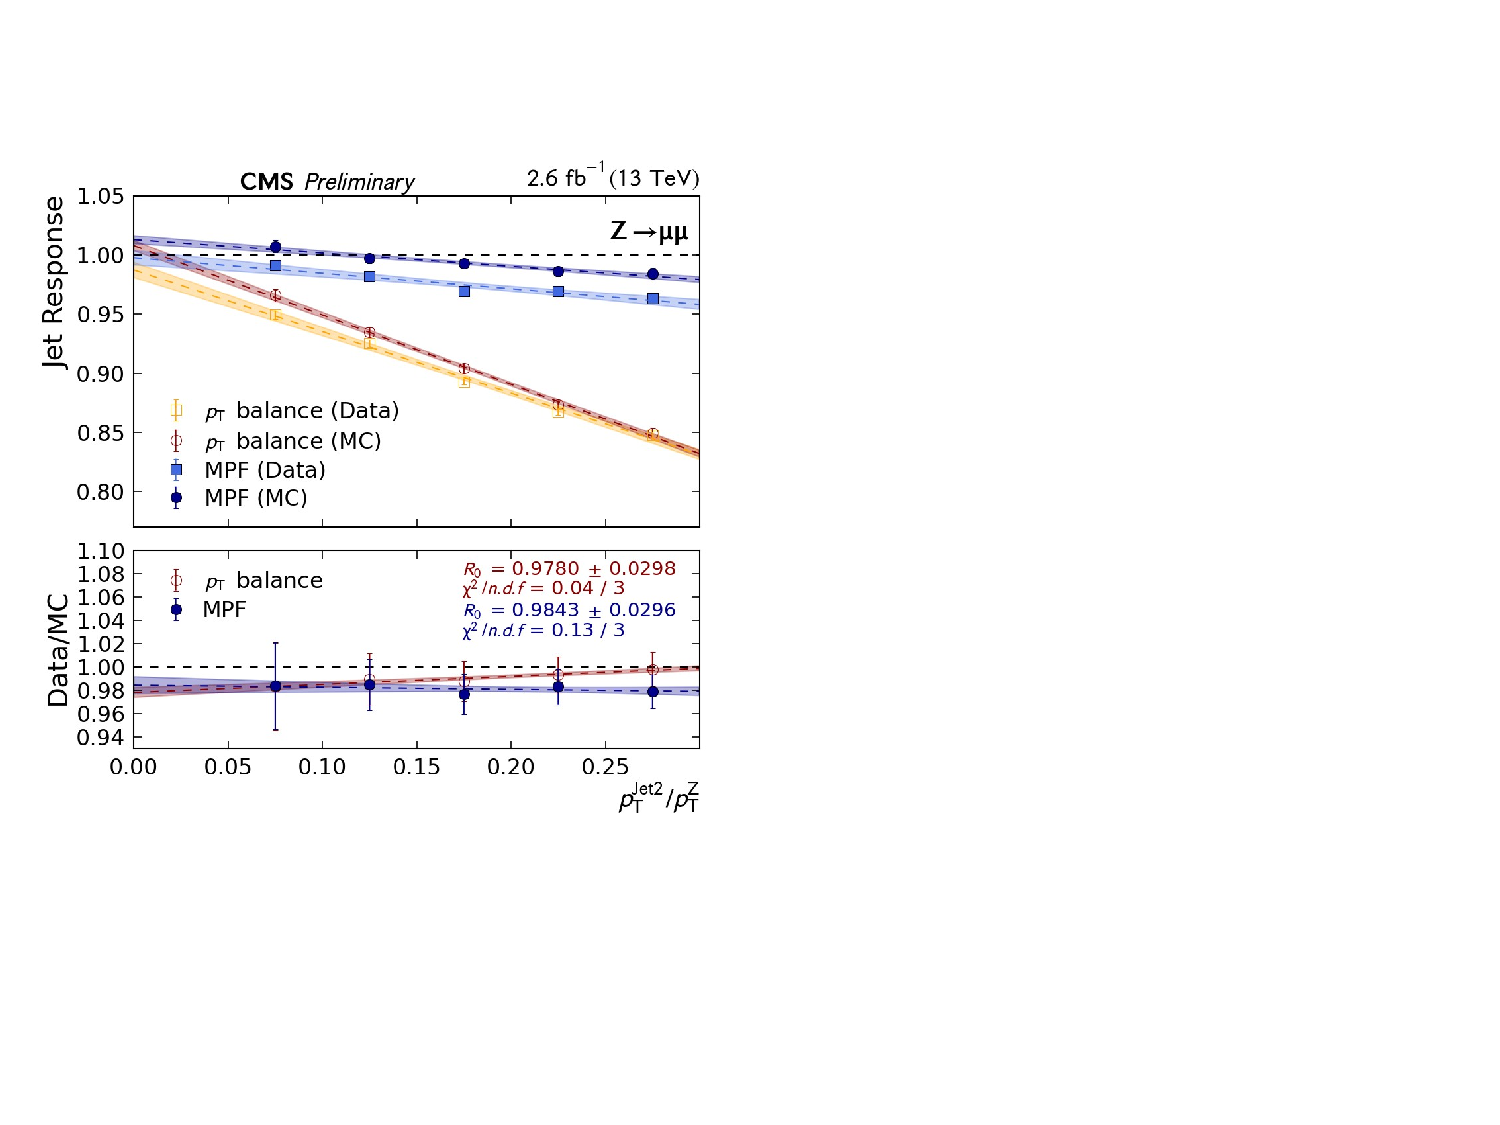
\includegraphics[width=.9\textwidth]{images/l3res.pdf}
				\label{fig:L3Residual}
		\end{figure}
		\vspace*{-0.6cm}
	\end{columns}
}
%%%%%%%%%%%%%%%%%%%%%%%%%%%%%%%%%%%%%%%%%%%%%%%%%%
%---------------------------------------------------------------------------------------------------------------------------------------
\frame{
	\frametitle{Global Fit}
	\vspace*{-0.24cm}
	\begin{columns}[T]
		\column{0.4\textwidth}
		\begin{block}{}
		  \begin{itemize}
		    \footnotesize
		  \item The final absolute jet $p_T$ scale is taken from a global fit to Z+jet, $\gamma$+jet, and multijet data
                  \item Essentially combines the different L3Residual methods ($p_T$ balance, $MPF$, $MJB$) and data samples
                  \item Covers full $p_T$ range and reduces uncertainty
                  \item On right, solid line shows central value and dotted lines show statistical uncertainty of the fit
		  \end{itemize}
		\end{block}
		\column{0.6\textwidth}
		\vspace*{-0.4cm}
		\begin{figure}[T]
		  \centering
		  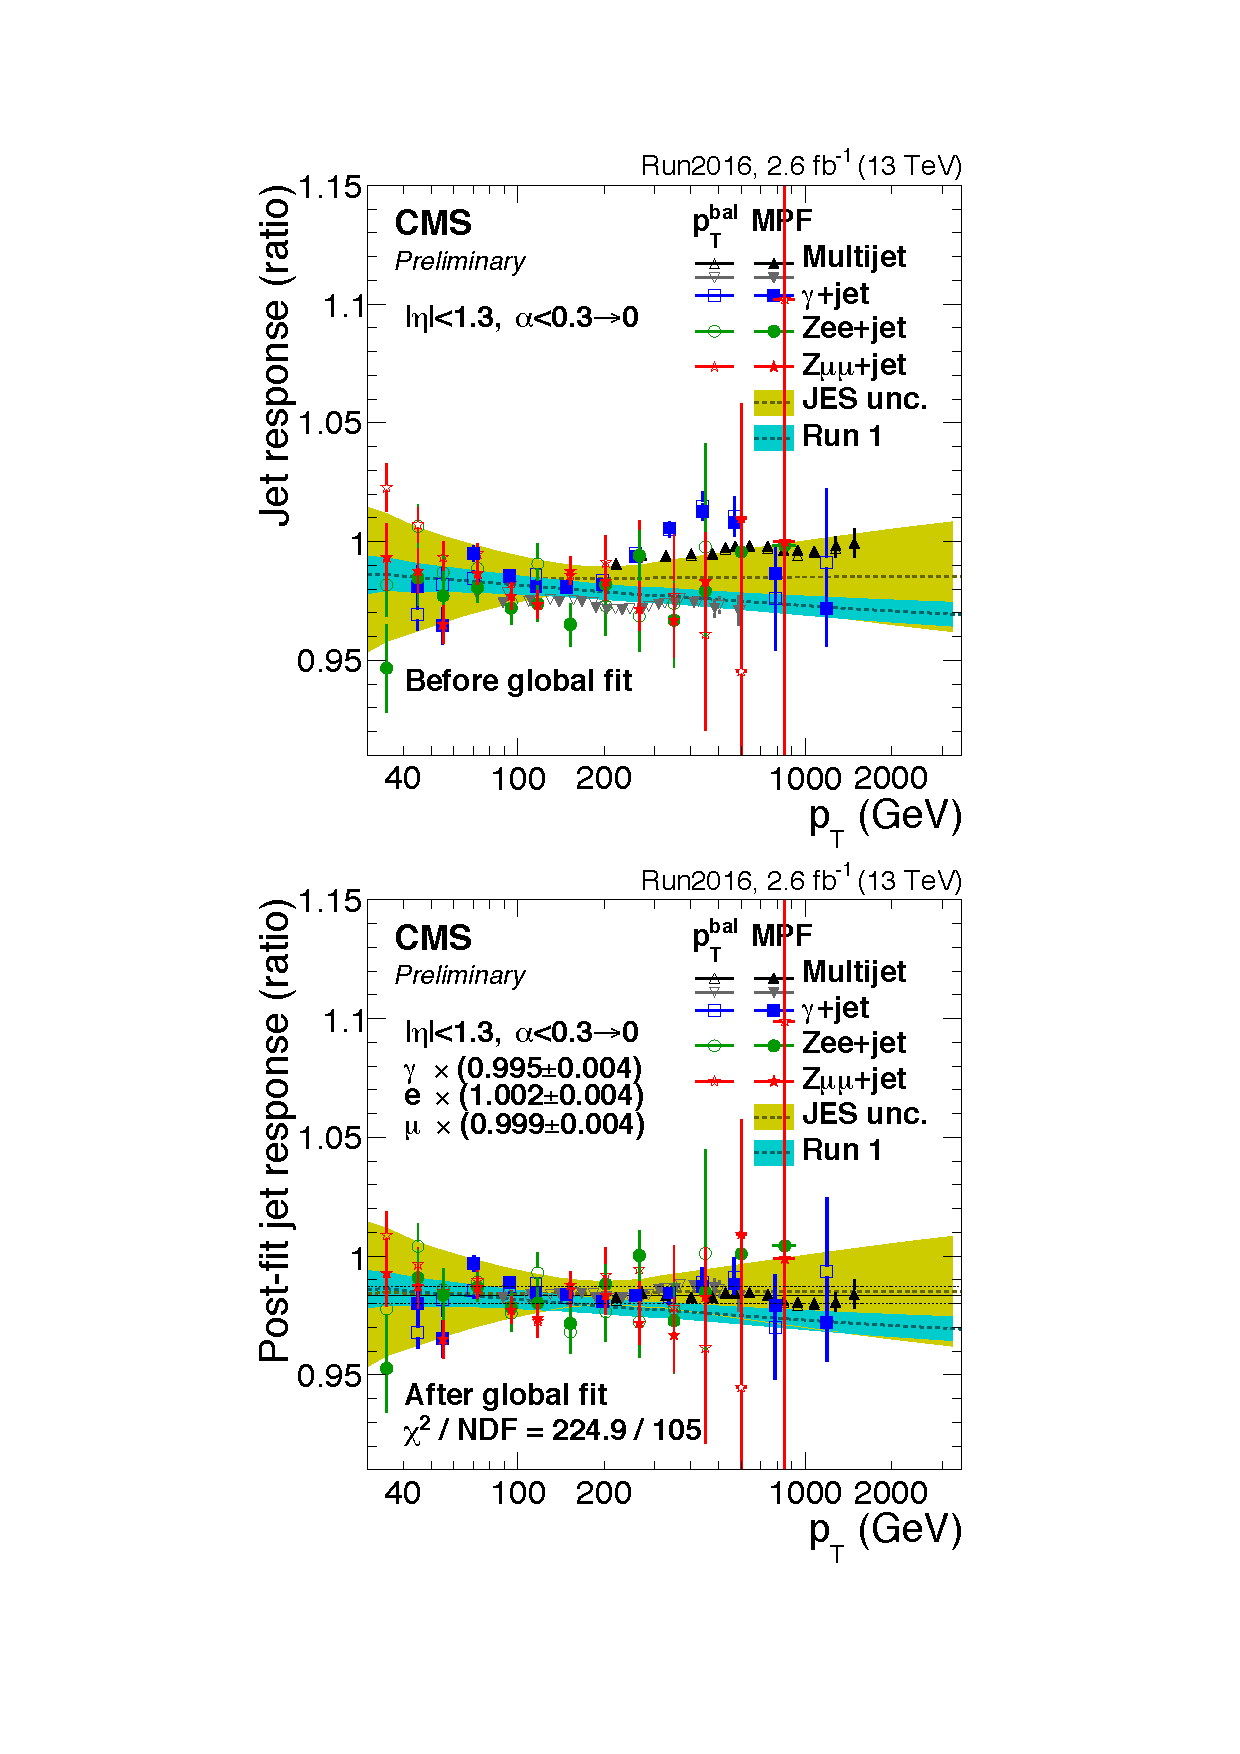
\includegraphics[width=.62\textwidth]{images/globalfit.pdf}
		  \label{fig:L3Residual}
		\end{figure}
		\vspace*{-0.6cm}
	\end{columns}
}
%%%%%%%%%%%%%%%%%%%%%%%%%%%%%%%%%%%%%%%%%%%%%%%%%%
\subsection{Uncertainties}
\frame{
	\frametitle{Many Sources of Uncertainty!}

        \begin{figure}[T]
          \centering
          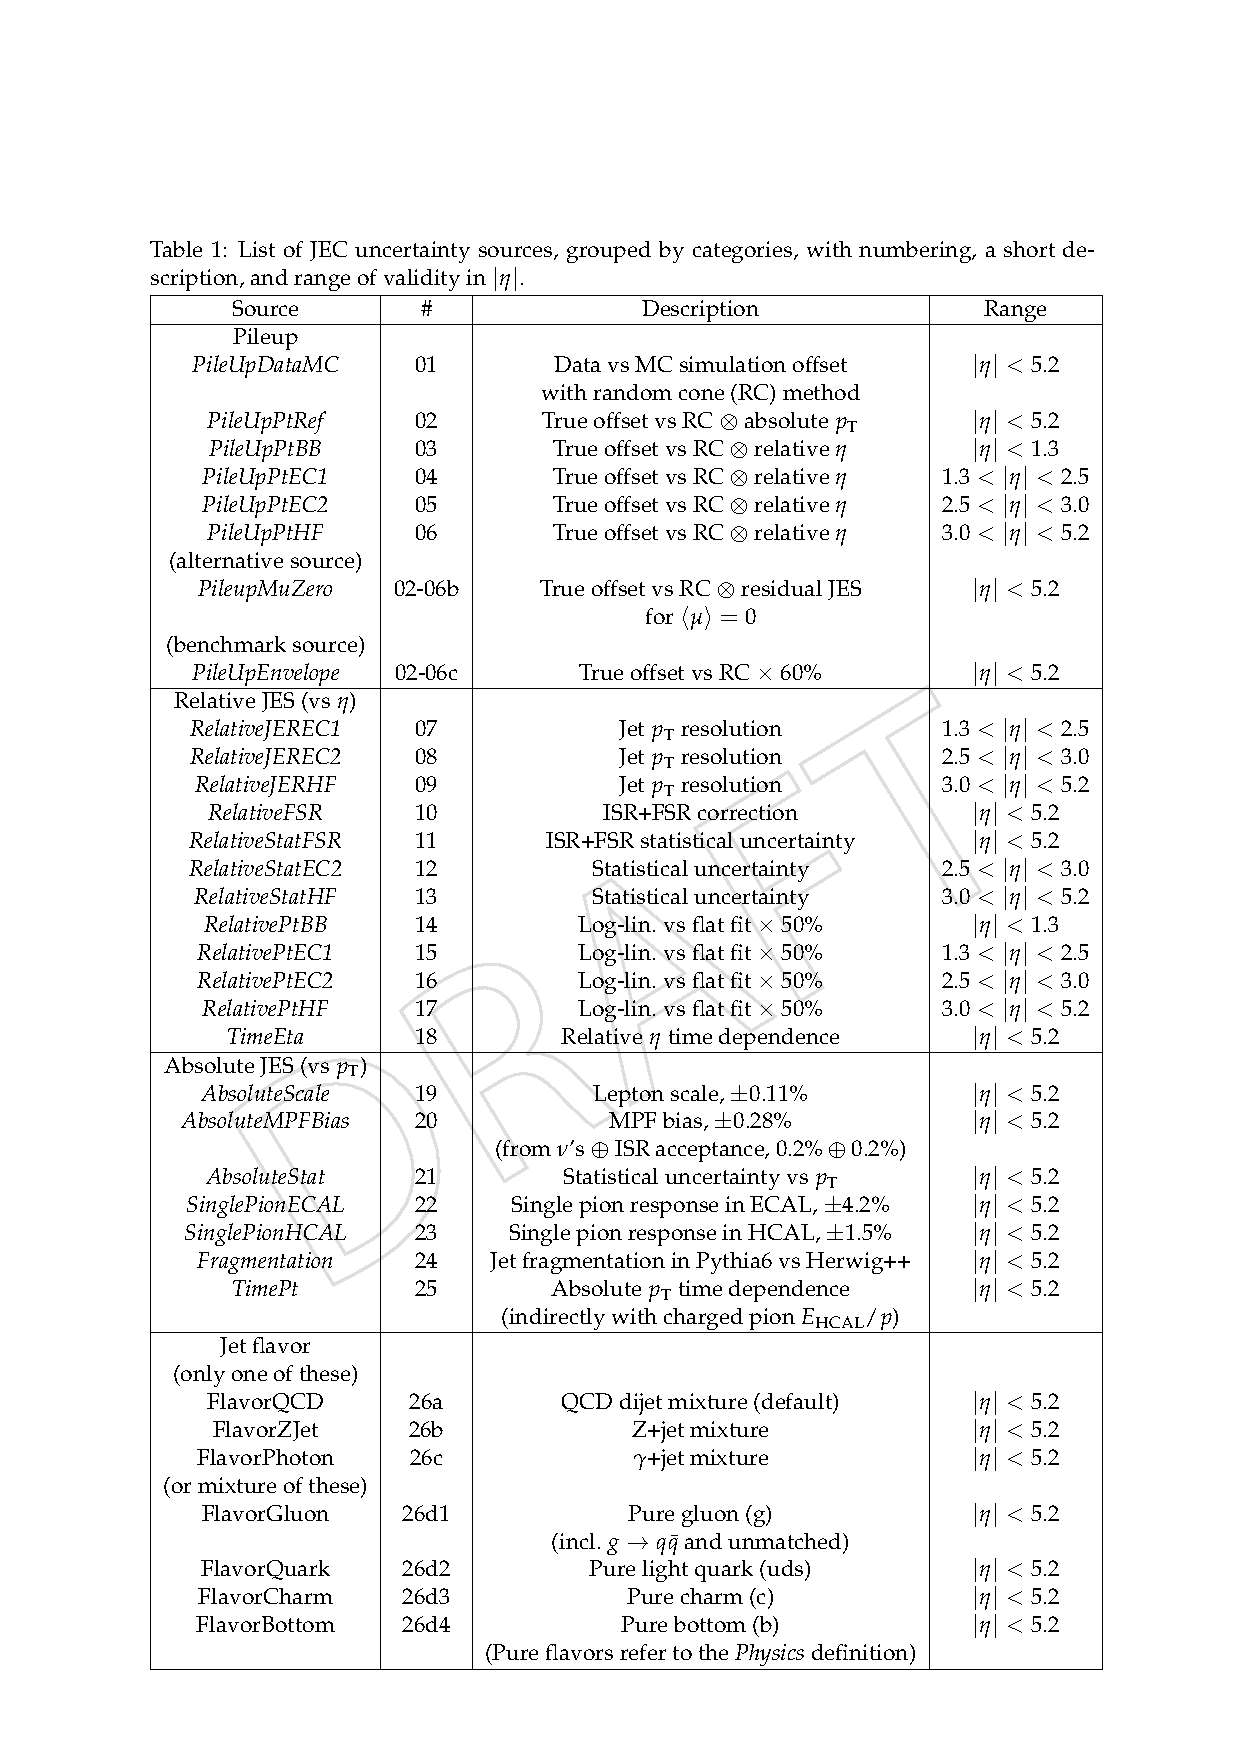
\includegraphics[width=.4\textwidth]{images/all_unc.pdf}
          \label{fig:all_unc}
        \end{figure}
        
}
%%%%%%%%%%%%%%%%%%%%%%%%%%%%%%%%%%%%%
%%%%%%%%%%%%%%%%%%%%%%%%%%%%%%%%%%%%%%%%%%%%%%%%%%
\subsection{Grouped Uncertainties}
\frame{
  \frametitle{Grouped Uncertainties}
  
  \begin{columns}
    \begin{column}{0.35\textwidth}
      \begin{block}{}
	\begin{itemize}
	\item Many sources of uncertainty
        \item Provided in special combinations specific to different analysis use cases (see table)
        \item Four broad categories (see plots)
          \begin{itemize}
            \item Absolute scale
            \item Relative $\eta$-dependent
            \item Pileup offset
            \item Flavor response differences
          \end{itemize}
          \item Can also allow for time dependence
	\end{itemize}
      \end{block}
    \end{column}
    \begin{column}{0.65\textwidth}
      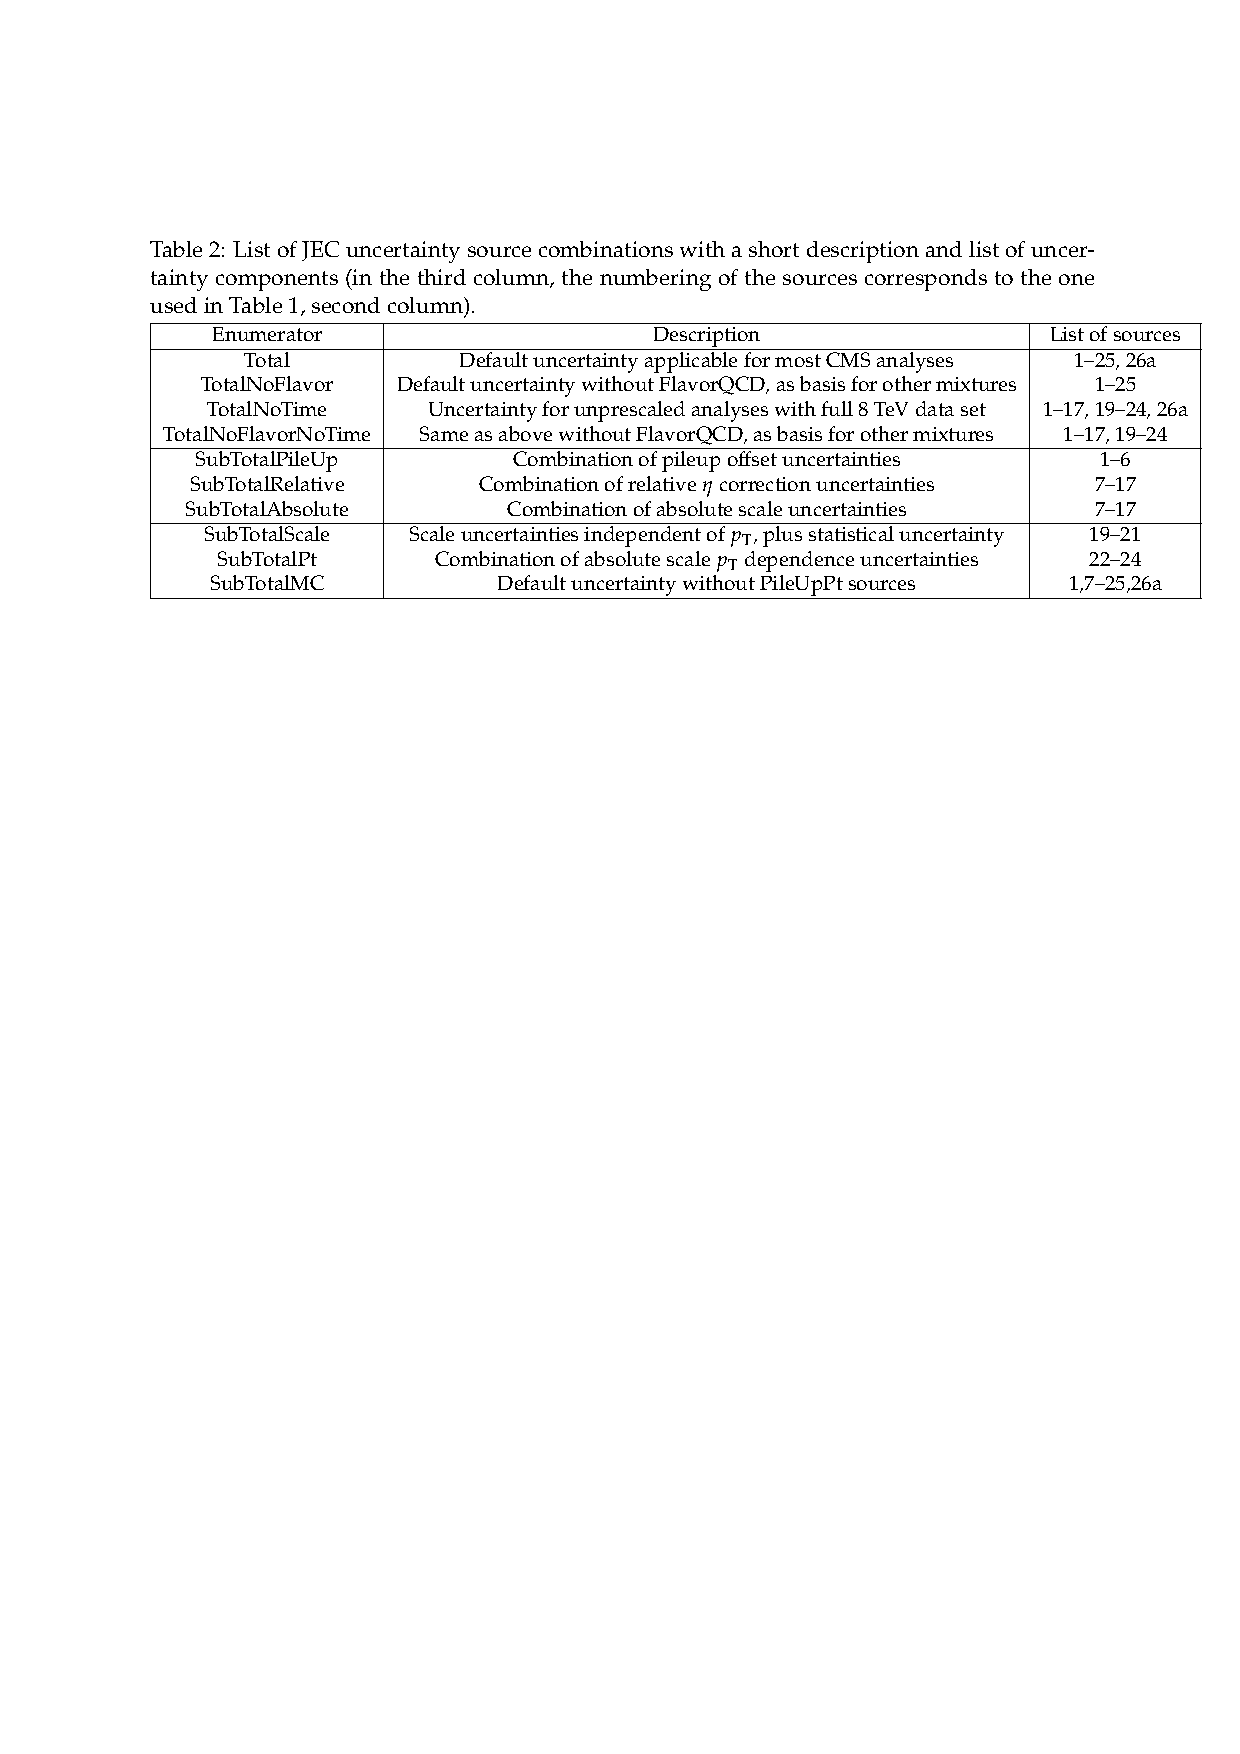
\includegraphics[width=\textwidth]{images/grouped_unc.pdf}\\
      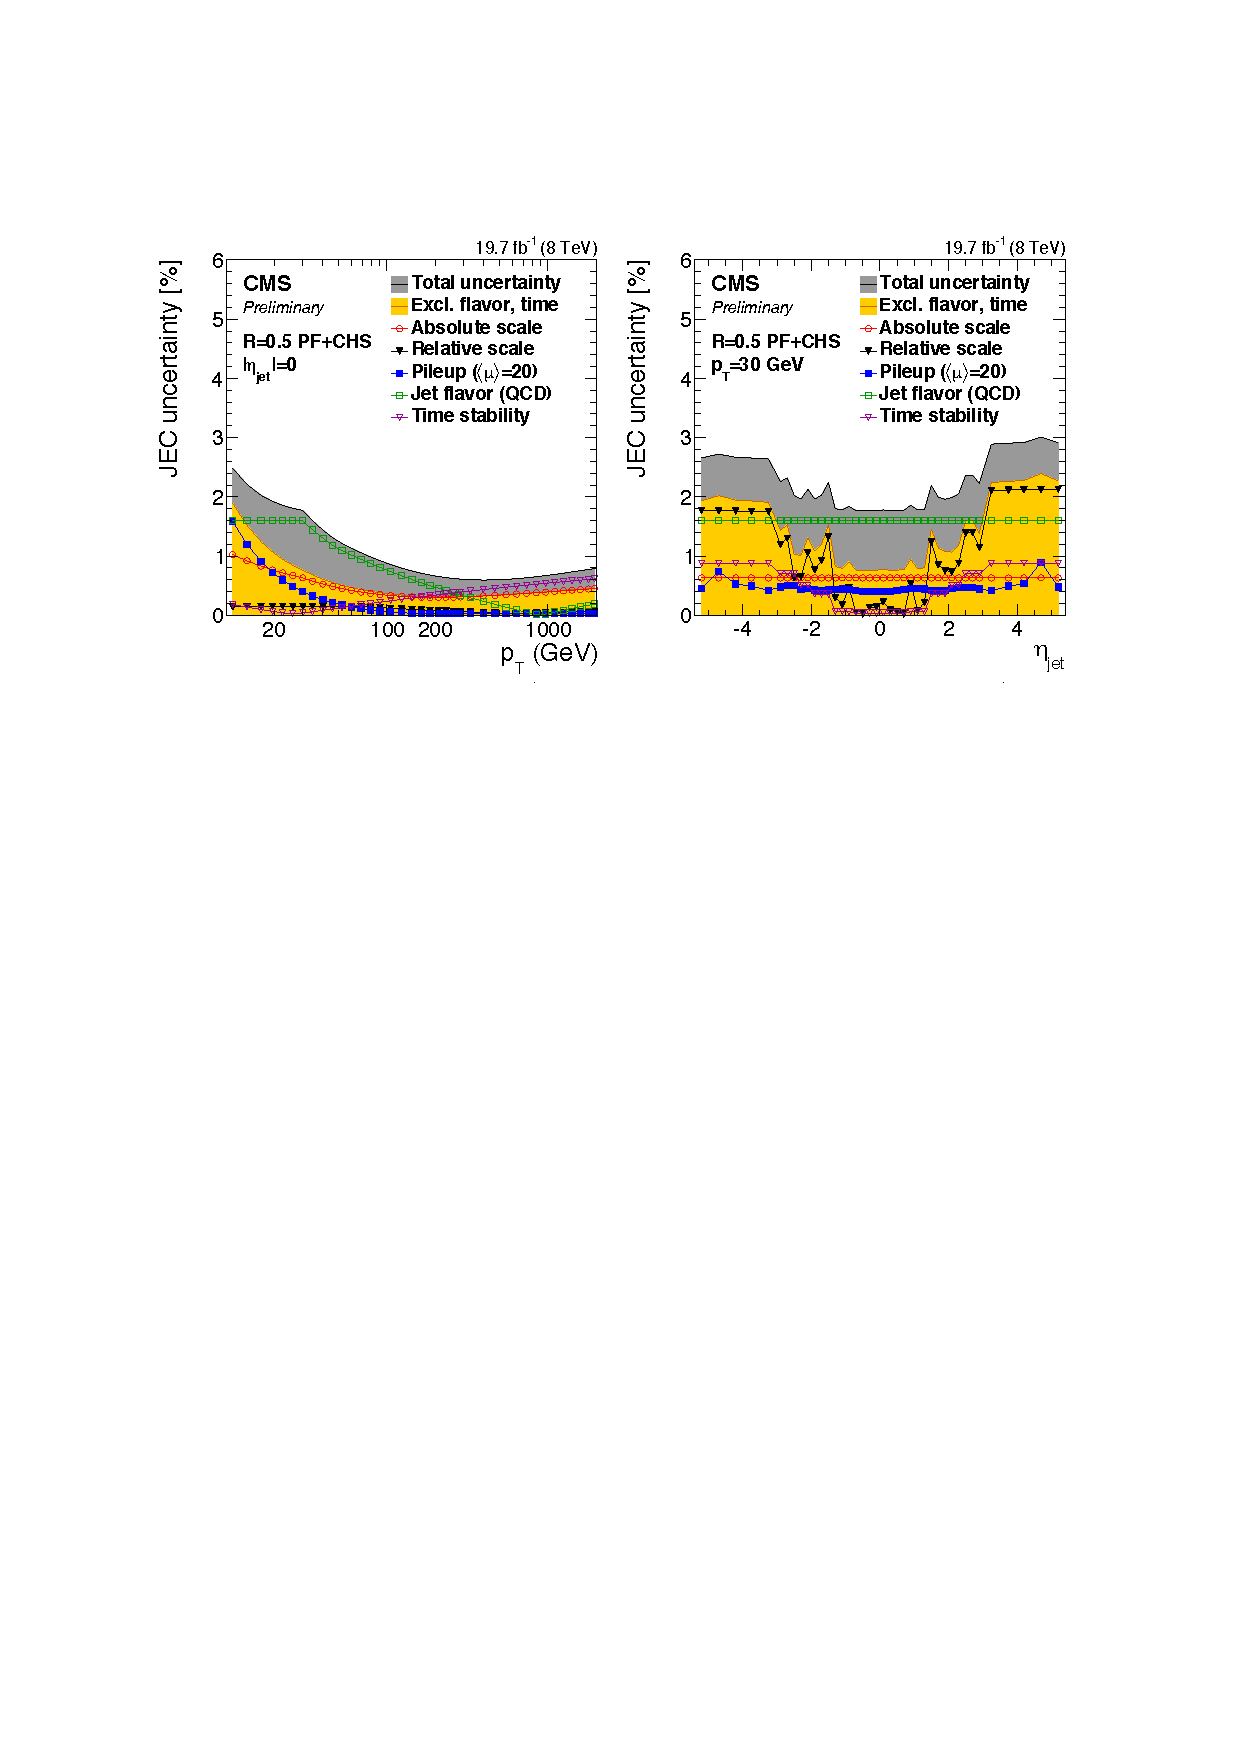
\includegraphics[width=\textwidth]{images/plot_unc.pdf}
    \end{column}
  \end{columns}
  
}
%%%%%%%%%%%%%%%%%%%%%%%%%%%%%%%%%%%%%%%%%%%%%%%%%%%%%%%%%%


%---------------------------------------------------------------------------------------------------------------------------------------
\frame{
\frametitle{Mandatory Jet Energy Corrections at CMS}
%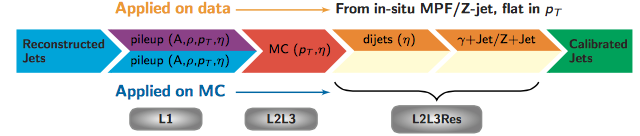
\includegraphics[width=10cm]{images/jecs.png}
\begin{itemize}
\item The minimum correction levels to be applied on any CMS analysis using Monte Carlo and Data are:

\begin{itemize}
\item \textbf{Monte Carlo:}\\
{\color{red}L1(Pile Up) + L2(Relative) + L3(Absolute)}
\item \textbf{Data:}\\
{\color{red}L1(Pile Up) + L2(Relative) + L3(Absolute) + L2L3 Residuals}
\end{itemize}
\item Any analysis might place higher correction levels if necessary and available. 
\item User can check \href{https://twiki.cern.ch/twiki/bin/view/CMS/JECDataMC}{https://twiki.cern.ch/twiki/bin/view/CMS/JECDataMC} to learn about the ``Recommended Jet Energy Corrections and Uncertainties for Data and MC".
\end{itemize}

}
%---------------------------------------------------------------------------------------------------------------------------------------
%\subsubsection{JER Uncertainty Sources}
%\frame{
%\frametitle{JES and Uncertainties}
%\begin{block}{Description}
%\begin{itemize}
%\item The JEC uncertainty sources provide detailed information on JEC uncertainties for use in statistical data analysis. The sources are fully uncorrelated between themselves, but describe JEC variations that are fully correlated within a given source.
%\item FIX ME: Should we include how uncertainties are calculated? How they are applied? Sources?
%\end{itemize}
%\end{block}
%}
%---------------------------------------------------------------------------------------------------------------------------------------
\subsection{Collections}
\frame{
	\frametitle{Jet Collections Supported by the JERC Group}
	\begin{itemize}
		\item Clustering algorithms:
		\begin{itemize}
			\item Anti-k$_{T}$
		\end{itemize}
		\item Cone sizes:
		\begin{itemize}
			\item R=0.4, 0.8
		\end{itemize}
		\item Jet types:
		\begin{itemize}
			\item PF - Still in use
			\item PF+CHS - Default
			\item PF+PUPPI - New kid on the block
			\item Calo 
			\item Jet Plus Track (JPT)
		\end{itemize}
	\end{itemize}
}
%---------------------------------------------------------------------------------------------------------------------------------------
%---------------------------------------------------------------------------------------------------------------------------------------

%---------------------------------------------------------------------------------------------------------------------------------------
